% Options for packages loaded elsewhere
\PassOptionsToPackage{unicode}{hyperref}
\PassOptionsToPackage{hyphens}{url}
%
\documentclass[
  11pt,
]{article}
\usepackage{amsmath,amssymb}
\usepackage{lmodern}
\usepackage{iftex}
\ifPDFTeX
  \usepackage[T1]{fontenc}
  \usepackage[utf8]{inputenc}
  \usepackage{textcomp} % provide euro and other symbols
\else % if luatex or xetex
  \usepackage{unicode-math}
  \defaultfontfeatures{Scale=MatchLowercase}
  \defaultfontfeatures[\rmfamily]{Ligatures=TeX,Scale=1}
\fi
% Use upquote if available, for straight quotes in verbatim environments
\IfFileExists{upquote.sty}{\usepackage{upquote}}{}
\IfFileExists{microtype.sty}{% use microtype if available
  \usepackage[]{microtype}
  \UseMicrotypeSet[protrusion]{basicmath} % disable protrusion for tt fonts
}{}
\makeatletter
\@ifundefined{KOMAClassName}{% if non-KOMA class
  \IfFileExists{parskip.sty}{%
    \usepackage{parskip}
  }{% else
    \setlength{\parindent}{0pt}
    \setlength{\parskip}{6pt plus 2pt minus 1pt}}
}{% if KOMA class
  \KOMAoptions{parskip=half}}
\makeatother
\usepackage{xcolor}
\usepackage[margin=1in]{geometry}
\usepackage{color}
\usepackage{fancyvrb}
\newcommand{\VerbBar}{|}
\newcommand{\VERB}{\Verb[commandchars=\\\{\}]}
\DefineVerbatimEnvironment{Highlighting}{Verbatim}{commandchars=\\\{\}}
% Add ',fontsize=\small' for more characters per line
\newenvironment{Shaded}{}{}
\newcommand{\AlertTok}[1]{\textcolor[rgb]{1.00,0.00,0.00}{\textbf{#1}}}
\newcommand{\AnnotationTok}[1]{\textcolor[rgb]{0.38,0.63,0.69}{\textbf{\textit{#1}}}}
\newcommand{\AttributeTok}[1]{\textcolor[rgb]{0.49,0.56,0.16}{#1}}
\newcommand{\BaseNTok}[1]{\textcolor[rgb]{0.25,0.63,0.44}{#1}}
\newcommand{\BuiltInTok}[1]{\textcolor[rgb]{0.00,0.50,0.00}{#1}}
\newcommand{\CharTok}[1]{\textcolor[rgb]{0.25,0.44,0.63}{#1}}
\newcommand{\CommentTok}[1]{\textcolor[rgb]{0.38,0.63,0.69}{\textit{#1}}}
\newcommand{\CommentVarTok}[1]{\textcolor[rgb]{0.38,0.63,0.69}{\textbf{\textit{#1}}}}
\newcommand{\ConstantTok}[1]{\textcolor[rgb]{0.53,0.00,0.00}{#1}}
\newcommand{\ControlFlowTok}[1]{\textcolor[rgb]{0.00,0.44,0.13}{\textbf{#1}}}
\newcommand{\DataTypeTok}[1]{\textcolor[rgb]{0.56,0.13,0.00}{#1}}
\newcommand{\DecValTok}[1]{\textcolor[rgb]{0.25,0.63,0.44}{#1}}
\newcommand{\DocumentationTok}[1]{\textcolor[rgb]{0.73,0.13,0.13}{\textit{#1}}}
\newcommand{\ErrorTok}[1]{\textcolor[rgb]{1.00,0.00,0.00}{\textbf{#1}}}
\newcommand{\ExtensionTok}[1]{#1}
\newcommand{\FloatTok}[1]{\textcolor[rgb]{0.25,0.63,0.44}{#1}}
\newcommand{\FunctionTok}[1]{\textcolor[rgb]{0.02,0.16,0.49}{#1}}
\newcommand{\ImportTok}[1]{\textcolor[rgb]{0.00,0.50,0.00}{\textbf{#1}}}
\newcommand{\InformationTok}[1]{\textcolor[rgb]{0.38,0.63,0.69}{\textbf{\textit{#1}}}}
\newcommand{\KeywordTok}[1]{\textcolor[rgb]{0.00,0.44,0.13}{\textbf{#1}}}
\newcommand{\NormalTok}[1]{#1}
\newcommand{\OperatorTok}[1]{\textcolor[rgb]{0.40,0.40,0.40}{#1}}
\newcommand{\OtherTok}[1]{\textcolor[rgb]{0.00,0.44,0.13}{#1}}
\newcommand{\PreprocessorTok}[1]{\textcolor[rgb]{0.74,0.48,0.00}{#1}}
\newcommand{\RegionMarkerTok}[1]{#1}
\newcommand{\SpecialCharTok}[1]{\textcolor[rgb]{0.25,0.44,0.63}{#1}}
\newcommand{\SpecialStringTok}[1]{\textcolor[rgb]{0.73,0.40,0.53}{#1}}
\newcommand{\StringTok}[1]{\textcolor[rgb]{0.25,0.44,0.63}{#1}}
\newcommand{\VariableTok}[1]{\textcolor[rgb]{0.10,0.09,0.49}{#1}}
\newcommand{\VerbatimStringTok}[1]{\textcolor[rgb]{0.25,0.44,0.63}{#1}}
\newcommand{\WarningTok}[1]{\textcolor[rgb]{0.38,0.63,0.69}{\textbf{\textit{#1}}}}
\usepackage{graphicx}
\makeatletter
\def\maxwidth{\ifdim\Gin@nat@width>\linewidth\linewidth\else\Gin@nat@width\fi}
\def\maxheight{\ifdim\Gin@nat@height>\textheight\textheight\else\Gin@nat@height\fi}
\makeatother
% Scale images if necessary, so that they will not overflow the page
% margins by default, and it is still possible to overwrite the defaults
% using explicit options in \includegraphics[width, height, ...]{}
\setkeys{Gin}{width=\maxwidth,height=\maxheight,keepaspectratio}
% Set default figure placement to htbp
\makeatletter
\def\fps@figure{htbp}
\makeatother
\setlength{\emergencystretch}{3em} % prevent overfull lines
\providecommand{\tightlist}{%
  \setlength{\itemsep}{0pt}\setlength{\parskip}{0pt}}
\setcounter{secnumdepth}{5}
\newlength{\cslhangindent}
\setlength{\cslhangindent}{1.5em}
\newlength{\csllabelwidth}
\setlength{\csllabelwidth}{3em}
\newlength{\cslentryspacingunit} % times entry-spacing
\setlength{\cslentryspacingunit}{\parskip}
\newenvironment{CSLReferences}[2] % #1 hanging-ident, #2 entry spacing
 {% don't indent paragraphs
  \setlength{\parindent}{0pt}
  % turn on hanging indent if param 1 is 1
  \ifodd #1
  \let\oldpar\par
  \def\par{\hangindent=\cslhangindent\oldpar}
  \fi
  % set entry spacing
  \setlength{\parskip}{#2\cslentryspacingunit}
 }%
 {}
\usepackage{calc}
\newcommand{\CSLBlock}[1]{#1\hfill\break}
\newcommand{\CSLLeftMargin}[1]{\parbox[t]{\csllabelwidth}{#1}}
\newcommand{\CSLRightInline}[1]{\parbox[t]{\linewidth - \csllabelwidth}{#1}\break}
\newcommand{\CSLIndent}[1]{\hspace{\cslhangindent}#1}
\usepackage{float} \usepackage{setspace} \usepackage[nottoc]{tocbibind} \usepackage{titlesec} \titleformat{\section}{\normalfont\LARGE\bfseries}{\thesection}{1em}{} \titleformat{\subsection}{\normalfont\Large\bfseries}{\thesubsection}{1em}{} \usepackage{pdflscape} \usepackage{fancyhdr} \usepackage{xcolor} \pagestyle{fancy} \fancyhf{} \fancyhead[R]{\textcolor{gray}{Variable Selection in High-Dimensional Data within the Bayesian Framework}} \renewcommand{\headrulewidth}{0.4pt} \renewcommand{\headrule}{\hbox to\headwidth{\color{gray}\leaders\hrule height \headrulewidth\hfill}} \renewcommand{\footrulewidth}{0pt} \usepackage{hyperref}
\usepackage{booktabs}
\usepackage{longtable}
\usepackage{array}
\usepackage{multirow}
\usepackage{wrapfig}
\usepackage{float}
\usepackage{colortbl}
\usepackage{pdflscape}
\usepackage{tabu}
\usepackage{threeparttable}
\usepackage{threeparttablex}
\usepackage[normalem]{ulem}
\usepackage{makecell}
\usepackage{xcolor}
\ifLuaTeX
  \usepackage{selnolig}  % disable illegal ligatures
\fi
\IfFileExists{bookmark.sty}{\usepackage{bookmark}}{\usepackage{hyperref}}
\IfFileExists{xurl.sty}{\usepackage{xurl}}{} % add URL line breaks if available
\urlstyle{same} % disable monospaced font for URLs
\hypersetup{
  hidelinks,
  pdfcreator={LaTeX via pandoc}}

\author{}
\date{\vspace{-2.5em}}

\begin{document}

\onehalfspacing

\begin{center}
  
  \textbf{\LARGE \textbf{Abstract}}
  
  \noindent 


This study examines challenges inherent in variable selection for linear models within the Bayesian framework, particularly in high-dimensional settings using R packages. 'High-dimensionality' refers to contexts involving many predictors that are fewer, equal to, or greater than the number of data points. Frequentist penalised regression Lasso and elastic-net methods and the machine learning XGBoost method are initially used to establish a benchmark. Subsequent Bayesian approaches encompass Bayesian Lasso, spike-and-slab prior, spike-and-slab Lasso, horseshoe priors, and the simplified shotgun stochastic search with screening. Packages that share methodologies are juxtaposed for user-friendliness and implementation nuances. Simulated data scenarios reveal that Bayesian methods, which compute coefficient credible intervals, often outperform frequentist counterparts by adeptly integrating model uncertainty into feature selection. However, they may miss weak signals when predictors significantly outnumber data points. Methods based on point estimates tend to retain irrelevant variables, while the machine learning method underperforms in all settings. Analysing socio-economic crime data largely aligns with the synthetic data study outcomes.

  \end{center}

\newpage

\section*{\LARGE Acknowledgements}

I am profoundly grateful to my advisor, Dr Michail Papathomas, whose
guidance was instrumental throughout my dissertation journey. His
insights and constructive feedback on my draft greatly contributed to my
work. My sincere appreciation goes to the Computer Science laboratory
for providing a conducive environment that promotes privacy and a
cheerful atmosphere, free from the constraints of societal norms. A
special mention goes to the new friends I have made over the last year -
their support has been invaluable, and they will forever hold a special
place in my heart. Finally, I would like to express my gratitude to the
beaches of St Andrews, whose breathtaking beauty was a constant source
of inspiration and tranquillity during this period.

\newpage

\subsection*{\LARGE Software and Code}

All analyses presented in this thesis were conducted using R software,
version 2022.12.0+353. The complete R code can be found in the Appendix
Code Section 10.3 for replication and further exploration. To execute
the analysis, initiate the `main.R' file. Ensure that other associated
files are sourced correctly within the `main.R' for seamless execution.

\newpage

\tableofcontents

\newpage

\listoffigures

\newpage

\listoftables

\newpage

\section{Introduction}

The personal motivation to delve into the intricacies of the Bayesian
statistical framework was kindled by Nobel laureate Daniel Kahneman's
seminal and highly digestible book `Thinking Fast and Slow'
(\protect\hyperlink{ref-Kahneman2011}{Kahneman, 2011}). Kahneman's
dissection of human cognitive biases and flawed decision-making,
especially in ambiguous situations, characterises System 1 thinking as
heuristic-driven, low-cost, and low-effort, often resulting in pitfalls
of emotionally induced biases. It is posited that the Bayesian
methodology parallels System 2 thinking, where prior beliefs are updated
with new evidence, considering the strength of the information. The
Bayesian approach provides an explicit mathematical framework for
handling uncertainty, counterbalancing overconfidence and confirmation
bias by quantifying uncertainties in light of new evidence.

Bayesian statistics employs probability distributions, constructed using
probability theory, to describe the `degree of belief'. Its strengths
and weaknesses simultaneously lie in the flexible incorporation of
background information. Arguably, it presents a more organic approach to
scientific reasoning than frequentist methods, updating beliefs with new
data. Relying only on data likelihood under specific hypotheses, without
prior beliefs, results in a rigid inference process. Priors become
especially valuable when data is limited; sometimes, they might be the
only available information. Even with a non-informative prior, Bayesian
methodology yields a distribution in contrast to the classical
approach's point estimate, making it, although subjectively, more
intuitively understandable.

Bayesian approaches elegantly circumvent challenges encountered by
classical methods. They sidestep issues of functional maximisation,
which eliminates problems with algorithm convergence and the delicate
task of choosing starting values close to the maximum
(\protect\hyperlink{ref-Train2012}{Train, 2012}). Further, Bayesian
methods alleviate the dilemma between local and global maxima, as
convergence does not inherently imply the attainment of a global
maximum. Moreover, they allow for desirable consistency and efficiency
under more forgiving conditions: consistency is achievable with a fixed
number of simulation draws, and any increase in draw numbers with sample
size ensures efficiency.

This thesis begins with an overview and reflection on personal interests
in Chapter 1. Chapter 2 details the motivation for high-dimensional
variable selection, while Chapter 3 delves into Bayesian inference
theory. Chapter 4 overviews linear regression and model selection across
frequentist and Bayesian paradigms. Chapter 5 expands on variable
selection techniques, encompassing frequentist, Bayesian, and machine
learning approaches. Chapter 6 showcases simulations and their outcomes,
leading into Chapter 7's deep dive into a crime dataset analysis.
Finally, Chapter 8 provides the conclusions of the research.

\newpage

\section{Motivation}

In data-driven decision-making, emphasis is on the abundance of data,
adhering to the principle that observations should outnumber explanatory
variables to prevent model overfitting and boost predictive power.
Technological advancements have accelerated scientific progress, leading
to vast data sets where variables often outnumber data points. A key
challenge in such high-dimensional settings is achieving sparsity,
ensuring model simplicity and interpretability without compromising
predictive accuracy, thus addressing the variance and overfitting issues
inherent in large datasets (\protect\hyperlink{ref-Hastie2017}{Hastie et
al., 2017}). For instance, while astronomy and image processing may have
thousands of noisy pixel observations, only a small subset is essential
to identify key objects (\protect\hyperlink{ref-Johnstone2004}{Johnstone
\& Silverman, 2004}). Meanwhile, data can be limited in medical research
on rare diseases or novel treatments. Here, the Central Limit Theorem
(CLT) might be invoked to assume data distribution, even if sample sizes
do not fully support the theorem's accuracy.

Variable selection seeks the optimal subset of predictors and
coefficients to drive the most fitting model for the data. However, it
is essential to remember that the `best' model does not claim to uncover
the absolute truth about the underlying natural processes, which are far
too intricate to be fully captured in mathematical terms
(\protect\hyperlink{ref-Ewout2019}{Steyerberg, 2019}). With unseen or
undiscovered predictors, and potential effects too minuscule to
empirically detect, statistical models remain valuable approximations,
drawing from the limited palette of known predictors to paint a feasible
picture of the complex reality. When the vector of regression
coefficients \(\beta\) is large and sparse, that is, most elements are
zero or negligible, identifying the significant elements of \(\beta\)
becomes particularly important (\protect\hyperlink{ref-Moran2019}{Moran
et al., 2019}). The goal is to identify a sparse subset of predictors
that adequately capture the true signals within the data, allowing for
the construction of parsimonious, interpretable models that effectively
mitigate overfitting (\protect\hyperlink{ref-Fan2008}{J. Fan \& Lv,
2008}).

Within classical statistics, specifically in high-dimensional contexts,
the non-uniqueness of solutions frequently arises. When predictors \(p\)
outnumber observations \(n\), the matrix \(X^TX\) often becomes singular
or nearly so (\protect\hyperlink{ref-Hastie2017}{Hastie et al., 2017}).
This results in ordinary least squares estimates for regression
coefficients that are unstable or undefined. One of the primary factors
exacerbating this issue is collinearity. Even when predictors are not
causally related, their high correlations can obfuscate the
interpretation of their individual effects on the response variable.
Such collinearity poses a significant challenge in high-dimensional
model selection (\protect\hyperlink{ref-Jianqing2010}{Jianqing et al.,
2010}). Moreover, it can be misleading in high-dimensional geometry,
potentially guiding statisticians towards an inaccurate model selection
(\protect\hyperlink{ref-Fan2008}{J. Fan \& Lv, 2008}). This environment
further amplifies the risk of overfitting.

In high-dimensional model building, addressing noise is crucial. Noisy
data, characterised by corruption or a low signal-to-noise ratio, can
skew results if not properly managed, leading to misleading conclusions.
While assuming a parametric form streamlines estimation, it might not
always capture the true underlying structure, risking inaccurate
estimates. Furthermore, highly flexible models, though adaptable, are
prone to overfitting, becoming more attuned to noise than to genuine
patterns (\protect\hyperlink{ref-Hastie2017}{Hastie et al., 2017}). Such
noise can compromise both the reliability and interpretability of a
model.

This thesis explores penalised regression methods within the frequentist
framework, addressing high dimensionality, collinearity, and noise
challenges. Penalised regression techniques impose penalties on
regression coefficients, promoting stability amidst collinearity and
high dimensionality. In contrast, Bayesian methods, while incorporating
priors for structured uncertainty modelling, stand out due to their
non-reliance on asymptotic results. As the sample size increases,
Bayesian inference capitalises on the asymptotic normality of the
posterior distribution, ensuring the parameter vector's posterior
distribution converges to multivariate normality for consistent and
efficient estimates (\protect\hyperlink{ref-Gelman2020}{Gelman et al.,
2020}). Machine learning technique Extreme Gradient Boosting (XGBoost)
utilise grid search, cross-validation, and tree number limitation to
optimise parameters, minimise prediction errors, and guard against
overfitting, noise, and spurious correlations. Whilst frequentist and
Bayesian methods often set their primary goal as drawing inference,
machine learning is often cited for its aim to predict. These methods
are defined in detail in subsequent chapters.

This analysis investigates high-dimensional linear regression variable
selection using both simulated data, where the number of predictors is
smaller, equal, greater or even much greater than the number of data
points, and the real data with many predictors and data points. The
study employs a mix of Bayesian methods, classical penalised regression,
and a gradient-boosted decision tree, all executed in R software. It
should be noted that some methodologies deployed in this study are not
the original versions but extensions found within the implemented
packages. This approach is intended to simplify the reader's narrative
and illuminate the adaptations required to overcome computational
limitations, enhance methodological efficiency and improve performance
outcomes. In doing so, this study provides insights into which
adjustments have proved most effective. Furthermore, comparative
analyses of different packages for some methodologies are undertaken to
compare user-friendliness and consistency.

The aims of this thesis extend beyond applying and comparing various
variable selection methods in linear regression problems. Equally
important is the personal journey into the depth of the Bayesian
statistical framework, as it remained unexplored during my studies.
Before my Master's in Applied Statistics and Data Mining, my academic
foundation was rooted in a creative discipline. Hence, this exploration
of statistical frameworks is a scholarly endeavour and a pivotal chapter
in my academic transition and growth. This document delivers definitions
of the methods, blending theory with application to foster a deep
understanding of the methodology and its practical testing.

\newpage

\section{Bayesian Framework: Building Blocks}

This thesis focuses on parametric models, characterised by a finite
number of parameters independent of the sample size, belonging to the
parameterised family of distributions. The number of parameters reflects
model complexity.

The steps involved in Bayesian inference methodology are outlined to
facilitate familiarity with the concepts:

\begin{enumerate}
\def\labelenumi{\arabic{enumi}.}
\item
  \emph{Development of a full Probability Model}: A joint probability
  distribution that encompasses all observable and latent variables is
  formulated. Ensuring the model is consistent with the prevailing
  understanding of the scientific problem and the data collection
  procedure is crucial.
\item
  \emph{Conditioning on Observed Data}: The posterior distribution is
  computed and analysed. The most common approach to posterior
  distribution computation is Markov Chain Monte Carlo (MCMC) and Gibbs
  Sampling. Given the observed data, this distribution represents the
  conditional probability of the latent variables of interest.
\item
  \emph{Assessment of Model Fit and Posterior Distribution
  Implications}: The model is evaluated, as are the plausibility of the
  substantive conclusions derived from the posterior distribution. The
  assessment also includes checking the conclusions' robustness and the
  results' sensitivity to the initial modelling assumptions. If
  necessary, the model is modified or expanded, and the process is
  iterated.
\end{enumerate}

\subsection{Foundations of Bayesian Inference}

This section relies on `Bayesian Analysis' lecture material by Fan,
Stanford University (\protect\hyperlink{ref-Fan2016}{2016}).

In the Bayesian framework, parameter \(\theta\) is modelled as a random
variable. This paradigm absorb prior beliefs about an unknown parameter
\(\theta\) and revises these beliefs upon observing new data. Prior to
observing any data, the unknown parameter is represented as a random
variable \(\Theta\) with a probability distribution
\(f_\Theta(\theta)\), known as the prior distribution (later denoted as
\(p(\theta)\)). This distribution embodies the initial beliefs about the
parameter's value.

Conditional on \(\Theta = \theta\), the observed data \(X\) is assumed
to follow the distribution \(f_{X|\Theta}(x|\theta)\). This distribution
characterises a parametric model parameterised by \(\theta\). The joint
distribution of \(\Theta\) and \(X\) is expressed as:

\begin{equation}
f_{X,\Theta}(x, \theta) = f_{X|\Theta}(x|\theta) f_\Theta(\theta)
\end{equation}

For continuous cases, the marginal distribution of \(X\) is given by:

\begin{equation}
f_X(x) = \int f_{X,\Theta}(x, \theta) d\theta = \int f_{X|\Theta}(x|\theta) f_\Theta(\theta) d\theta
\end{equation}

The conditional distribution of \(\Theta\) given \(X = x\) is defined
as:

\begin{equation}
f_{\Theta|X}(\theta|x) = \frac{f_{X|\Theta}(x|\theta) f_\Theta(\theta)}{\int f_{X|\Theta}(x|\theta') f_\Theta(\theta') d\theta'}
\end{equation}

This equation is derived using Bayes' theorem, which relates the
posterior distribution, the likelihood, and the prior distribution.
Specifically, the numerator represents the product of the likelihood and
the prior, while the denominator ensures normalisation.
\(f_{\Theta|X}(\theta|x)\) (later presented as \(\pi(\theta|x)\)) is
termed the posterior distribution of \(\Theta\), representing our
updated understanding of the parameter \(\Theta\) after observing data
\(X\). Concisely, it can be articulated as:

\begin{equation}
\begin{aligned}
    f_{\Theta|X}(\theta|x) &\propto f_{X|\Theta}(x|\theta) f_\Theta(\theta) \label{eq:posterior} \\
    \text{Posterior density} &\propto \text{Likelihood} \times \text{Prior density} 
\end{aligned}
\end{equation}

where the posterior density is proportional to the product of the
likelihood and the prior density. The symbol \(\propto\) masks the
proportionality factor
\(f_X(x) = \int f_{X|\Theta}(x|\theta') f_\Theta(\theta') d\theta'\),
which is independent of \(\theta\).

The \emph{prior distribution} represents our knowledge or beliefs about
a parameter before observing any data. Priors can be categorised as
either `informative' or `uninformative'. `Informative' priors are
derived from sources such as additional data, insights from experts, or
elicitation methods (\protect\hyperlink{ref-Dias2017}{Dias et al.,
2017}). On the other hand, uninformative priors are typically broad or
non-committal distributions, serving as placeholders in the absence of
strong prior beliefs (examples include uniform or Jeffreys' priors)
(\protect\hyperlink{ref-Price2002}{Price \& Manson, 2002}). Prior
selection will play a crucial role for variable selection in this
thesis.

The likelihood function \(f_{X|\Theta}(x|\theta)\), later presented as
\(p(x|\theta)\), evaluates how probable the observed data \(x\) is under
various parameter values \(\theta\). Unlike the prior distribution, the
likelihood function depends solely on the data and quantifies its
support for various parameter values. The likelihood function is not a
probability distribution over \(\theta\), that is, it does not provide
probabilities for different parameter values but rather gives a measure
of how well each parameter value \(\theta\) is supported by the data.

The \emph{posterior distribution} synthesises all available information
regarding the parameter of interest. However, deriving analytical
summaries, such as the posterior distribution's mean, variance, credible
intervals, or inclusion probabilities often requires evaluating complex
integrals. The evaluation can be incredibly challenging for
high-dimensional posterior distributions. Monte Carlo integration, a
simulation technique, offers an effective solution for estimating these
integrals. Within the Monte Carlo framework, the Markov Chain Monte
Carlo (MCMC) methodology is a powerful tool for approximating all these
posterior summary statistics. The application of this methodology is
defined in the following section.

\subsection{MCMC Algorithm}

The following description lays the foundation of \emph{Markov Chain
Monte Carlo (MCMC)} algorithms, of which three are particularly
prominent: Gibbs sampling, Metropolis-Hastings, and Importance/Rejection
sampling.

\emph{MCMC} involves generating samples of \(\theta\) from approximate
distributions and iteratively refining these samples to converge to the
desired posterior distribution, \(\pi(\theta|x)\). The essence of
\emph{MCMC} is not the Markov property per se but the progressive
improvement of the approximation towards the target distribution with
each iteration. A Markov chain is defined as a stochastic sequence
\(\{\theta^0, \theta^1, \theta^2, \ldots, \theta^n\}\), where each state
\(\theta^n\) depends only on its immediate predecessor \(\theta^{n-1}\),
where the initial state \(\theta^0\) is set to an arbitrary value. The
Markov chain evolves according to a transition kernel \(P\), dependent
only on \(\theta^n\):

\begin{equation}
\theta^{n+1} \sim P(\theta^n, \theta^{n+1}) \, (\equiv P(\theta^{n+1}|\theta^n)).
\end{equation}

Given the conditions of aperiodicity and irreducibility, a Markov chain
will converge to a stationary distribution that does not depend on its
initial values. In practical applications, determining the exact point
of convergence is challenging. The initial states of the chain, which
might not accurately represent the posterior distribution, are typically
discarded in a process known as `burn-in'
(\protect\hyperlink{ref-Brooks1998}{Brooks \& Gelman, 1998}). This
ensures that the chain has sufficiently converged to a stable mean.
Various techniques, including trace plots
(\protect\hyperlink{ref-Plummer2005}{Plummer et al., 2005}) and the
Brooks-Gelman-Rubin (BGR) method
(\protect\hyperlink{ref-Brooks1998}{Brooks \& Gelman, 1998}), help
ascertain the burn-in length. BGR method uses an analysis of variance to
assess the similarity of estimates from different starting points.

Once the burn-in phase is complete, it is crucial to have an adequate
number of iterations to ensure accurate summary statistics and minimal
Monte Carlo errors. A common approach to estimating the Monte Carlo
error involves batching. The chain is divided into \(m\) batches, each
of length \(T\), so that \(n = mT\). Let \(\theta_1,\ldots,\theta_m\) be
the sample means for each batch, and \(\theta\) denote the mean overall
\(n\) samples. The batch means estimate of \(\sigma^2\) is then,

\begin{equation}
\hat{\sigma}^2 = \frac{T}{m - 1} \sum_{i=1}^{m}(\bar{\theta}_i - \bar{\theta})^2.
\end{equation}

An estimate of the Monte Carlo error is
\(\sqrt{\frac{\hat{\sigma}^2}{n}}\). The efficiency of the Markov chain
in exploring the parameter space can be evaluated using the
autocorrelation function (ACF). The ACF is the correlation of a
parameter's value in the Markov chain with itself at a lag \(j\),
defined as \(\text{cor}(\theta^t, \theta^{t+j})\). Efficient chains show
a fast decrease in ACF as the lag increases, indicating low dependency
between chain values within a few iterations.

An alternative estimate of the Monte Carlo error uses the effective
sample size \(M\), defined as

\begin{equation}
M = \frac{n}{1 + 2 \sum_{k=1}^{\infty} \rho_k},
\end{equation}

where \(\rho_k\) is the autocorrelation at lag \(k\). Practically, \(M\)
is estimated through an alternative method accounting for
autocorrelations. The Monte Carlo error can be estimated as
\(\sqrt{\frac{\hat{\sigma}^2}{\hat{M}}}\).

Finally, `thinning' in the context of \emph{MCMC} refers to selecting
every \(k_{th}\) realisation from the chain, discarding the rest. This
process helps reduce the autocorrelation within the sampled sequence.
While thinning can be beneficial, especially in memory-constrained
situations, it should be used judiciously. By discarding samples,
valuable information might be lost.

Section 4.5 will introduce the Reversible Jump MCMC method, an advanced
extension of \emph{MCMC} that involves Gibbs sampling, which is the most
relevant to this paper.

\newpage

\section{Model Selection Methodology}

\subsection{The Setting: Linear Regression Model}

The thesis explores the multiple linear regression model within the
frequentist statistical framework, described as

\begin{equation}
\mathbf{Y} = \beta_0 + \mathbf{X}\boldsymbol{\beta} + \boldsymbol{\epsilon}, \quad \boldsymbol{\epsilon} \sim \mathcal{N}(\mathbf{0}, \sigma^2\mathbf{I}_n).
\end{equation}

Here, \(\mathbf{Y} \in \mathbb{R}^n\) is the response vector,
\(\beta_0\) is the intercept, \(\mathbf{X} \in \mathbb{R}^{n \times p}\)
is the design matrix comprising \(p\) potential predictors. The vector
\(\boldsymbol{\beta} = (\beta_1, ..., \beta_{p})^T \in \mathbb{R}^{p}\)
represents the set of regression coefficients that will be estimated.
The noise vector \(\boldsymbol{\epsilon} \in \mathbb{R}^n\) is
constituted by independently distributed normal random variables, each
sharing a common but unknown variance \(\sigma^2\). The term
\(\mathbf{I}_n\) denotes the \(n \times n\) identity matrix, ensuring
that the noise components are uncorrelated and have constant variance.

Transitioning to the Bayesian framework, the likelihood becomes:

\begin{equation}
\mathbf{Y} | \alpha, \boldsymbol{\beta}, \sigma^2 \sim \mathcal{N}_n(\mathbf{1}_n \alpha + \mathbf{X} \boldsymbol{\beta}, \sigma^2 \mathbf{I}_n),
\end{equation}

where the term \(\mathbf{1}_n \alpha\) creates a vector of length \(n\)
where every element is the intercept \(\alpha\).

In Bayesian regression, parameters \(\alpha\), \(\boldsymbol{\beta}\),
and \(\sigma^2\) are treated as random variables with respective prior
distributions:

\begin{equation}
\begin{aligned}
\boldsymbol{\beta} &\sim \pi(\boldsymbol{\beta}), \\
\alpha &\sim \pi(\alpha), \\
\sigma^2 &\sim \pi(\sigma^2).
\end{aligned}
\end{equation}

This thesis discusses methods for assessing the relative quality of
statistical models, including the Akaike information criterion (AIC) and
Watanabe--Akaike information criterion (WAIC). While the analysis
focuses on variable selection, the task of model selection is closely
related, and some of the applied R packages use these criteria (for
example, \emph{`spikeslab'} calculates AIC criteria, \emph{`bayesreg'} -
WAIC), warranting their brief explanation for methodological
completeness and personal understanding.

\subsection{AIC}

The following three sections draw from `Bayesian Data Analysis' by
Gelman et al. (\protect\hyperlink{ref-Gelman2020}{2020}).

In classical statistics, parameter \(\theta\) is typically inferred
using a point estimate, denoted as \(\hat{\theta}\), rather than the
full posterior distribution. The maximum likelihood estimate (MLE) is
often used as this point estimate. MLE determines the parameter values
of a statistical model that maximise the likelihood of observing the
given data. A common approach for calculating out-of-sample predictive
accuracy involves using the log posterior density of the observed data
\(x\) given the point estimate, \(\log p(x|\hat{\theta})\), and
correcting overfitting bias. When \(k\) represents the number of
estimated parameters, the bias penalisation is performed by subtracting
\(k\) from the log predictive density based on the MLE, according to the
formula:

\begin{equation}
\widehat{elpd}_{\text{AIC}} = \log p(x|\hat{\theta}_{\text{mle}}) - k.
\end{equation}

\emph{AIC} is then defined as twice the negative of this quantity:

\begin{equation}
\text{AIC} = -2 \log p(x|\hat{\theta}_{\text{mle}}) + 2k.
\end{equation}

AIC favours models that predict well and penalises models with excessive
parameters to discourage overfitting. Though \emph{AIC's} bias
correction, under certain assumptions, is applicable in normal linear
models with known variance and uniform priors, it is inadequate in
Bayesian models. In such cases, the penalty of \(k\) does not accurately
represent the effective number of parameters. Hence, other criteria were
introduced.

\subsection{WAIC}

\emph{WAIC} requires Monte Carlo estimation and is complex to implement
but offers a fully Bayesian approach to estimate out-of-sample
expectations (\protect\hyperlink{ref-Spiegelhalter2014}{Spiegelhalter et
al., 2014}). This method calculates the log pointwise posterior
predictive density and incorporates a correction for the effective
number of parameters to prevent overfitting.

Here, the robust WAIC modification is explored. The effective number of
parameters, \(p_{WAIC2}\), is derived from the variance of individual
terms in the log predictive density across all data points \(n\) as

\begin{equation}
p_{WAIC2} = \sum_{i=1}^{n} \text{var}_{\text{post}}(\log p(x_i|\theta)).
\end{equation}

Using the sample variance definition, the total variance across all data
points is computed to obtain the effective number of parameters. Then to
correct for bias:

\begin{equation}
\widehat{\text{elppd}}_{\text{WAIC}} = \text{lppd} - \text{p}_{\text{WAIC}}.
\end{equation}

Finally, similar to AIC and DIC, the WAIC is determined by:

\begin{equation}
WAIC = -2\text{lppd} + 2\text{p}_{WAIC2},
\end{equation}

where \(lppd\) is the computed log pointwise predictive density, derived
from the average of the predictive densities across all data points.

Unlike \emph{AIC}, which gauges the plug-in predictive density's
performance, \emph{WAIC} assesses predictions for new data in a Bayesian
context by averaging over the posterior distribution. While \emph{AIC},
and \emph{WAIC} aim to estimate the expected out-of-sample deviance of a
model, akin to versions of cross-validation, Bayesian Information
Criterion (BIC) focuses on approximating the marginal probability
density of the data under the model, pertinent in the context of
discrete model comparison (\protect\hyperlink{ref-Neath2012}{2012}).

\subsection{Bayes Factor and Reversible Jump Monte Carlo}

The \emph{Bayes factor}, introduced by Jeffrey
(\protect\hyperlink{ref-jeffreys1935}{1935}), is a key tool in
traditional Bayesian model comparison, widely discussed in Bayesian
literature. It quantifies the relative evidence for two models, \(M_i\)
and \(M_j\), given data \(x\),

\begin{equation}
B_{ij} = \frac{p(x|M_i)}{p(x|M_j)} = \frac{\int p(x|\theta_i,M_i)p(\theta_i|M_i)d\theta_i}{\int p(x|\theta_j,M_j)p(\theta_j|M_j)d\theta_j},
\end{equation}

where \(p(x|\theta_k,M_k)\) denotes the likelihood under model \(k\),
and \(p(\theta_k|M_k)\) represents the prior distribution of
\(\theta_k\). The variable \(M\) denotes the model, taking values from a
finite set of \(K\) models. \emph{Bayes factors} can be derived from
posterior model probabilities with known prior model probabilities
(\protect\hyperlink{ref-Kass1995}{Kass \& Raftery, 1995}), enabling
Bayesian model averaging, which accounts for model uncertainty in
posterior estimates (\protect\hyperlink{ref-Hoeting1999}{Hoeting et al.,
1999}).

Evaluating \emph{Bayes factors} is challenging due to the difficulty
computing marginal likelihoods for each model. MCMC methods offer a
solution but necessitate careful handling of varying parameter numbers
to ensure ergodicity in the Markov chain. Green's
(\protect\hyperlink{ref-Green1995}{1995}) \emph{Reversible Jump MCMC
(RJMCMC)} employs auxiliary variables to manage model dimension changes.
Defining pseudo-priors or auxiliary variables remains a challenging area
of ongoing research. Barker \& Link
(\protect\hyperlink{ref-Barker2013}{2013}) introduced a simplified
\emph{RJMCMC} approach, extending the Metropolis-Hastings algorithm to
allow the Markov chain to traverse varying dimensions. This methodology,
further developed by Gelling, Schofield, and Barker
(\protect\hyperlink{ref-Gelling2019}{2019}), is encapsulated in the
\emph{`rjmcmc'} package, facilitating Bayes factor and posterior model
probability calculations using \emph{RJMCMC} outputs.

Given data \(x\) with models indexed \(1,...,K\), and a set of
model-specific parameters \(\theta_k\) for each model \(k\), along with
prior model probabilities \(p(M_k)\), the posterior model probabilities
are related to Bayes factors as:

\begin{equation}
\frac{p(M_i|x)}{p(M_j|x)} = B_{ij} \times \frac{p(M_i)}{p(M_j)}
\end{equation}

\emph{RJMCMC} enables sampling across models by considering the model
indicator as a latent variable sampled using MCMC. The transition
between models \(i\) and \(j\) necessitates that: both models have an
equal number of parameters, and a bijective mapping exists between the
parameters of the two models. Auxiliary variables \(u_i\) are introduced
to ensure the dimensions match, that is,
\(\text{dim}(\theta_i,u_i) = \text{dim}(\theta_j,u_j)\). With the
freedom to transition between any pair of models, \(K(K-1)/2\)
bijections must be defined. The choice of auxiliary variables and
bijections does not alter the posterior distribution but affects
computational efficiency. Limiting transitions between models can reduce
the number of required bijections. During the \(t\) iteration of the
Markov chain, a proposed model \(M_{j}^*\) is introduced, while the
current value is denoted as \(M_{i}^{(t-1)}\). For model \(M_{j}^*\),
the proposed parameter values are determined using the bijection
\(f_{ij}(\cdot)\) as

\begin{equation}
(\theta_{j}^*, u_{j}^*) = f_{ij}(\theta_{i}^{(t-1)}, u_{i}^{(t-1)}).
\end{equation}

The joint proposal is accepted or rejected using a Metropolis step. The
selection of the bijection is crucial, as it affects the efficiency and
convergence rate of the chain. The restricted version of \emph{RJMCMC}
involves introducing a universal parameter vector \(\psi\), whose
dimension is at least the maximum dimension of the model-specific
parameters, that is,

\begin{equation}
\text{dim}(\psi) \geq \max_{k} \{\text{dim}(\theta_{k})\}.
\end{equation}

Model-specific parameters \(\theta_i\) and auxiliary variables \(u_i\)
are derived from \(\psi\) using a bijection \(g_i(\cdot)\):

\begin{equation}
(\theta_{i}, u_{i}) = g_{i}(\psi),
\end{equation}

\begin{equation}
\psi = g_{i}^{-1}(\theta_{i}, u_{i}).
\end{equation}

Model parameters in model \(i\) are mapped to model \(j\) through the
universal parameter vector \(\psi\),

\begin{equation} 
\begin{split}
(\theta_{j}, u_{j}) &= g_{j}(\psi) \\
                    &= g_{j}(g_{i}^{-1}(\theta_{i}, u_{i})).
\end{split}
\end{equation}

This method necessitates \(K\) bijections to move among \(K\) models.
The joint distribution is expressed as:

\begin{equation}
p(y,\psi,M_k)=p(y|\psi,M_k)p(\psi|M_k)p(M_k),
\end{equation}

where \(p(y|\psi,M_k)=p(y|\theta_k,M_k)\) is the joint probability
density for the data under model \(k\), \(p(\psi|M_k)\) is the prior for
\(\psi\) given model \(k\), and \(p(M_k)\) is the prior model
probability for model \(k\).

Since priors are typically in the form \(p(\theta_k|M_k)\),
\(p(\psi|M_k)\) is found as: \begin{equation}
p(\psi|M_k) = p(g_k(\psi)|M_k) \left| \frac{\partial g_k(\psi)}{\partial \psi} \right|,
\end{equation}

where \(\left| \frac{\partial g_k(\psi)}{\partial \psi} \right|\)is the
determinant of the Jacobian for the bijection \(g_k\), later denoted as
\(|J_k|\). The algorithm employs a Gibbs sampler that alternates between
updating \(M\) and \(\psi\). The full-conditional distribution for \(M\)
is categorical, with probabilities:

\begin{equation}
p(M_k|\cdot) = \frac{p(y,\psi,M_k)}{\sum_j p(y,\psi,M_j)}.
\end{equation}

A sample from the full-conditional for \(\psi\) is obtained by drawing
\(\theta_k\) and \(u_k\) from their respective distributions and
computing \(\psi=g_k^{-1}(\theta_k,u_k)\). Barker and Link
(\protect\hyperlink{ref-Barker2013}{2013}) also detailed a
Rao-Blackwellized estimator for posterior model probabilities based on
estimating a transition matrix whose \((i, j)\) entry represents the
probability of transitioning from model \(M_i\) to \(M_j\). The
posterior model probabilities are derived by normalising the left
eigenvector of this estimated transition matrix. An essential feature of
the \emph{`rjmcmc'} package is the automatic computation of \(|J_k|\)
through automatic differentiation, which greatly simplifies
implementation, especially when dealing with many parameters.

The \emph{`rjmcmc'} package facilitates precise estimation of Bayes
factors and posterior model probabilities for a predefined set of
models. While the original Green's \emph{RJMCMC}
(\protect\hyperlink{ref-Green1995}{1995}) is a versatile algorithm,
allowing parameter changes in MCMC simulations, the \emph{`rjmcmc'}
package is tailored to refine posterior distributions and facilitate
model comparison. Notably, it only permits transitions between models
with equal parameters. Comprehensive domain knowledge of the
socio-economic data analysed in later chapters is necessary, including
the ability to pre-select variables, a requirement that could not be
met. Prioritising established methodologies ensured reliability in the
findings of this dissertation.

\newpage

\section{Variable Selection Methodology}

\subsection{Frequentist Penalised Regression}

In penalised regression methods, a penalty term is added to the
log-likelihood function to enforce a trade-off between bias and variance
in regression coefficients, consequently optimising prediction error.

\emph{Least Absolute Shrinkage and Selection Operator (Lasso)}
incorporates the L1-norm, originally proposed by Tibshirani
(\protect\hyperlink{ref-Tibshirani1996}{1996}), of regression
coefficients (excluding the intercept) as the penalty term:

\begin{equation}
- \log L + \lambda \sum_{j=1}^{p} |\beta_j|, \quad \lambda > 0.
\end{equation}

This penalisation shrinks coefficients toward zero and sets those with a
negligible predictive contribution to zero, serving as an embedded
feature selection method. \emph{Lasso} does not group predictors, often
arbitrarily selecting one from a group of highly correlated predictors.

\emph{Ridge regression} employs the L2-norm of regression coefficients
(excluding the intercept) as the penalty:

\begin{equation}
- \log L + \lambda \sum_{j=1}^{p} \beta_j^2, \quad \lambda > 0.
\end{equation}

\emph{Ridge regression} shrinks coefficients towards zero but retains
all predictors in the model. When \(n > p\) and there is high
multicollinearity, \emph{Ridge regression} often offers superior
predictions. Since the penalty term is the sum of squared coefficients,
shrinkage would be unfair across predictors with different scales.
Hence, they need to be standardised.

\emph{Elastic-Net} combines the L1-norm and L2-norm penalties, the
method first proposed by Zou and Hastie
(\protect\hyperlink{ref-Zou2005}{2005}):

\begin{equation}
- \log L + \lambda_1 \sum_{j=1}^{p} |\beta_j| + \lambda_2 \sum_{j=1}^{p} \beta_j^2, \quad \lambda_1, \lambda_2 > 0.
\end{equation}

The combination of penalties can also be expressed as:

\begin{equation}
\lambda \left( \alpha \sum_{j=1}^{p} |\beta_j| + \frac{1-\alpha}{2} \sum_{j=1}^{p} \beta_j^2 \right), \quad \lambda > 0, \ 0 \leq \alpha \leq 1.
\end{equation}

Here, \(\alpha\) controls the mixing of \emph{Lasso} and \emph{Ridge}
penalties, and \(\lambda\) regulates the overall strength of
regularisation, see Figure 1.

\begin{figure}

{\centering \includegraphics[width=1\linewidth]{reg_pen} 

}

\caption{Contours of the Residual Sum of Squares (RSS) and Constraint Functions for Penalised Regression Techniques. Lasso (left), Ridge (centre), and Elastic-Net (right). Note: The shaded regions represent the constraint boundaries, blue ellipses depict the RSS contours.}\label{fig:penalisation graphics}
\end{figure}

Despite its proven efficacy, the original \emph{Lasso} method has
certain constraints. Tibshirani
(\protect\hyperlink{ref-Tibshirani1996}{1996}) noted that ridge
regression surpasses \emph{Lasso} when dealing with multicollinearity
among predictors. In situations with more predictors, \(p\), than
observations, \(n\), Lasso's convex optimisation limits it to selecting
no more than \(n\) variables. Moreover, it disregards meaningful feature
ordering and struggles to effectively select highly correlated grouped
variables, tending to choose individual ones instead. Later, Meier, Van
De Geer and Bühlmann (\protect\hyperlink{ref-Meier2008}{Meier et al.,
2008}) introduced algorithms designed for extremely high-dimensional
problems to solve convex optimisation issues. They demonstrated that the
group \emph{Lasso} estimator for logistic regression remains
statistically consistent with a sparse true underlying structure, even
when the number of predictors significantly outnumbers the observations.

The \emph{`glmnet'} package in R provides generalised linear model
fitting, allowing for Lasso or elastic-net regularisation with a
spectrum of lambda values, and includes capabilities for prediction,
plotting, and cross-validation, even for sparse datasets. Ten k-fold
cross-validations are used to determine \(\lambda\), which controls the
overall strength of the penalty in the \emph{`glmnet'} package under the
Lasso (\(\alpha = 1\)) or the elastic-net (\(alpha = 0.5\)) penalties.

\subsection{Machine Learning}

Exploring variable selection methods and comparing frequentist and
Bayesian inference approaches with a renowned machine learning method,
\emph{Extreme Gradient Boosting (XGBoost)}, would offer valuable
insights. \emph{XGBoost} introduced by Chen and Guestrin
(\protect\hyperlink{ref-Chen2016}{2016}) is often cited for outstanding
performance in Kaggle competitions. The method incorporates a feature
importance mechanism, which, in simple terms, quantifies the
contribution of individual attributes to the construction of decision
trees within the ensemble (\protect\hyperlink{ref-Chen2016}{Chen \&
Guestrin, 2016}).

\emph{XGBoost} boasts exceptional scalability, enabling rapid processing
on single machines and adept scaling to billions of examples in
memory-constrained environments. As a comprehensive tree-boosting
system, it introduces innovations such as a sparsity-aware algorithm for
sparse data and a theoretically grounded weighted quantile sketch for
handling instance weights, effectively streamlining resource employment
in processing large datasets (\protect\hyperlink{ref-Chen2016}{Chen \&
Guestrin, 2016}).

The following methodology is based on Wang, Xu, Zhao, Peng and Wang's
definition (\protect\hyperlink{ref-Wang2019}{2019}).

The \emph{XGBoost} model:

\begin{equation}
\hat{y_i} = \sum_{k=1}^{K} f_k(x_i), \quad f_k \in \mathcal{F}
\end{equation}

where \(\hat{y}_i\) is the predicted value for the \(i\)-th instance,
\(K\) denotes the number of trees, \(\mathcal{F}\) denotes the set of
all possible regression trees, and \(f_k\) represents a specific
regression tree.

The goal of \emph{XGBoost} is to build a \(K\) regression tree such that
the predictions of the tree group are as close as possible to the true
values while ensuring the greatest generalisation ability. The
prediction process is achieved by minimising an objective function,
given by:

\begin{equation}
\text{obj}(\theta) = \sum_{i}^{n} l(y_i, \hat{y}_i) + \sum_{k=1}^{K} \Omega(f_k),
\end{equation}

where the first component, \(\sum_{i=1}^{n} l(y_i, \hat{y}i)\), is a
loss function that measures the deviation of the predicted values from
the true values; the second part, \(\sum_{k=1}^{K} \Omega(f_k)\), acts
as a regularisation term that controls the complexity of the model, as:

\begin{equation}
\Omega(f_k) = \gamma T + \frac{1}{2} \lambda \lVert w \rVert^2,
\end{equation}

where \(T\) represents the number of leave nodes in the tree, and
\(\lVert w \rVert^2\) is the weight of the corresponding leaf nodes.

During the \(t\)-th iteration of training, the objective function is
defined as:

\begin{equation}
\text{obj}^{(t)} = \sum_{i=1}^{n} l\left(y_i, \hat{y}_i^{(t-1)} + f_t(x_i)\right) + \Omega(f_k) + \sum_{i=1}^{t-1} \Omega(f_i)
\end{equation}

This formulation encapsulates each tree's training error and complexity,
steering the algorithm toward building an ensemble of trees that
effectively balances accuracy and generalisation.

Figure 2 illustrates the tree-boosting process based on Guo et al.
(\protect\hyperlink{ref-Guo2020}{2020}).

\begin{figure}[H]

{\centering \includegraphics[width=0.9\linewidth]{xgboost_flow} 

}

\caption{XGBoost Algorithm. Iterative Tree Building Process}\label{fig:XGBoost flow}
\end{figure}

The \emph{XGBoost} model, known for its accuracy and resistance to
overfitting (\protect\hyperlink{ref-Wang2019}{Wang et al., 2019}),
supports weak classification and regression models. Although its
efficacy in classification is recognised, its use in high-dimensional
settings is debated (\protect\hyperlink{ref-Li2020}{Li, 2020}). In this
study, the real dataset being investigated comprises a scenario where
the number of data points exceeds the number of features, albeit with a
large feature space. It is essential to incorporate an additional
augmented simulated dataset configuration defined in Section 6.1.
Additionally, Adebisi (\protect\hyperlink{ref-Li2020}{2020}) highlighted
potential difficulties faced by \emph{XGBoost} when tasked with linear
regression with a continuous target. Notably, the majority of studies
employing this method focus on classification rather than linear
regression problems. This topic is delved into further in the
Conclusions chapter. To note, it is sensitive to outliers, too
(\protect\hyperlink{ref-Dairu2021}{Dairu \& Shilong, 2021}).

This thesis employs the \emph{XGBoost} model to calculate feature
importance, ranking variables by their significance in building boosted
trees. Features with non-zero importance scores are selected, typically
encompassing most covariates. The top variables are identified by
aggregating the gain, focusing on features contributing to 80\% of the
total gain, in line with the Pareto principle.

In the analysis, a grid search optimises hyperparameters, including
boosting rounds (50, 100, 150), tree depth levels (3, 5, 7, 9), learning
rates (0.01, 0.1, 0.3), and minimum loss reduction values (0, 0.1, 1).
Column subsample ratios during tree construction are set at 0.6, 0.8,
and 1, with minimum instance weight in a child node at 1, 3, and 5.
Training instance subsample ratios are 0.8 and 1. A 5-fold
cross-validation, repeated thrice, is used. The model focuses on linear
regression, with performance assessed by the Root Mean Square Error
(RMSE) during tuning.

\subsection{Bayesian Framework}

\subsubsection{Bayesian Lasso}

The Lasso, a frequentist penalised regression approach, aims to minimise
the Residual Sum of Squares (RSS) subject to the non-differentiable
constraint on the coefficients using the L1-norm, expressed as:

\begin{equation}
\min_{\beta} \left(\tilde{y} - X\beta \right)^T \left(\tilde{y} - X\beta \right) + \lambda \sum_{j=1}^{p} |\beta_j|
\end{equation}

where \(\tilde{y} = y - \bar{y}1_n\) for some \(\lambda \geq 0\).

Tibshirani (\protect\hyperlink{ref-Tibshirani1996}{1996}) interpreted
the Lasso estimates as Bayes posterior mode under individual Laplace
priors for each predictor. The Laplace distribution's ability to
manifest as a scale mixture of normal distributions with independently
exponentially distributed variances offers advantages. It prompted
several researchers to adopt Laplace priors within a hierarchical
Bayesian framework. This thesis discusses the one the \emph{`monomvn'}
package implements. Park and Casella
(\protect\hyperlink{ref-Casella2008}{2008}) proposed Gibbs sampling for
the Lasso, incorporating a Laplace prior within the hierarchical model.
They considered a fully Bayesian analysis using a conditional Laplace
prior as:

\begin{equation}
\pi(\beta|\sigma^2) = \prod_{j=1}^{p} \frac{\lambda}{2\sigma} e^{-\lambda|\beta_j|/\sigma}
\end{equation}

where the noninformative, scale-invariant marginal prior is
\(\pi(\sigma^2) = \frac{1}{\sigma^2}\). The conditioning on \(\sigma^2\)
asserts that it secures a unimodal full posterior. A lack of unimodality
can hinder the convergence of the Gibbs sampler, thus rendering point
estimates less reliable.

Park and Casella (\protect\hyperlink{ref-Casella2008}{2008}) argue that
the \emph{Bayesian Lasso} offers a middle ground between Lasso and Ridge
regression by providing smooth paths similar to Ridge but with a
tendency to push less significant parameters towards zero faster, akin
to Lasso. This behaviour suggests an edge of the Laplace prior over
Gaussian or Student-t priors in rapidly diminishing weakly related
parameters. However, this becomes an issue when the method is tasked
with variable selection, as the weakly related predictors would become
not precisely zero but only relatively small. The Bayesian Lasso employs
a double-exponential (Laplace) prior on the regression coefficients,
leading to the coefficients' shrinkage towards zero, refer to Figure 3.

\begin{figure}[H]

{\centering \includegraphics[width=0.75\linewidth]{dissertation_files/figure-latex/Bayesian Lasso Priors-1} 

}

\caption{Density Plots of Laplace Prior Distributions for Bayesian Lasso: Impact of tau}\label{fig:Bayesian Lasso Priors}
\end{figure}

The \emph{'monomvn'} package employs the Bayesian Lasso model via the
Gibbs Sampling algorithm from Park and Casella
(\protect\hyperlink{ref-Casella2008}{2008}). It introduced a feature to
use a Rao-Blackwellized sample of \(\sigma^2\), with \(\beta\)
integrated out, to improve the mixing of the sampling algorithm. A
unique part of this package is the inclusion of RJMCMC (default) for
Bayesian model selection and averaging, which allows users to determine
the best model based on the columns of the design matrix and their
corresponding \(\beta\) parameters. Unlike Hans
(\protect\hyperlink{ref-Hans2009}{2009}) and Geweke
(\protect\hyperlink{ref-Geweke1996}{1996}) methods, which require a
specific prior on each \(\beta_i\) and individual conditional sampling,
this implementation maintains joint sampling from the full \(\beta\)
vector of non-zero entries, thus facilitating better Markov chain
mixing. It also allows RJ proposals to alter the count of non-zero
entries on a component-wise basis, with high acceptance rates due to
marginalised between-model moves.

To apply the \emph{Bayesian Lasso} model, users set the initial Lasso
penalty parameter square, \(\lambda_{2}\); default is 1. For a
conservative approach, a burn-in of 1,000 samples is used, with
inference drawn from the subsequent 5,000 samples. Variable
normalisation is disabled; data is manually standardised as outlined in
Section 6.2. Other hyperparameters are left as default. Variables with
an inclusion probability over 0.5 are considered significant.

\subsubsection{Spike-and Slab Prior}

The \emph{spike-and-slab} approach was initially pioneered by Lempers
(\protect\hyperlink{ref-Lempers1971}{1971}), Mitchell, and Beauchamp
(\protect\hyperlink{ref-Mitchell1988}{Mitchell \& Beauchamp, 1988}). The
term `spike-and slab' refers to a two-component mixture prior used for
\(\beta\). This prior was set such that the \(\beta_k\) elements were
mutually independent, consisting of a flat uniform distribution (the
slab) and a zero degenerate distribution (the spike). See Figure 4
illustrating two samples drawn from normal distributions, representing
the `spike' and the `slab'. The `spike' represents a sample from a
distribution with a small standard deviation, mirroring the zero
degenerate distribution in the \emph{spike-and-slab} prior. The `slab'
is a sample drawn from a distribution with a large standard deviation,
representing the flat, uniform distribution in the prior.

\begin{figure}[H]

{\centering \includegraphics[width=0.75\linewidth]{dissertation_files/figure-latex/Spike Slab Priors-1} 

}

\caption{Density Plots of Three Spike-and-Slab Variants}\label{fig:Spike Slab Priors}
\end{figure}

Ishwaran and Rao (\protect\hyperlink{ref-Ishwaran2005}{2005}) proposed a
departure from this design. Instead of a two-component mixture, they
posited a multivariate normal scale mixture distribution for \(\beta\),
dictated by the prior \(\pi\) for the hypervariance \(\gamma\). Despite
the divergence in distribution choice, the core principle paralleled the
original methodology, aiming to shrink truly zero \(\beta_k\)
coefficients via small posterior mean values. The hypervariances played
a vital role in this, with smaller values driving coefficient shrinkage
and larger ones inflating coefficients for final model selection.

In further developing the \emph{spike-and-slab} model, Ishwaran and Rao
(\protect\hyperlink{ref-Ishwaran2005}{2005}) introduced a continuous
bimodal prior in a rescaled model variant. The use of such a flexible
prior helps to alleviate calibration challenges. To prevent the
diminishing influence of the prior on the posterior as the sample size
increases, they proposed a modification: a sample size invariant or
`universal' rescaling of the \emph{spike-and-slab} model. This
modification entails transforming the original \(Y_i\) values by a
factor of \(\sqrt{n}\) and incorporating a variance inflation factor to
compensate for the altered variance of the transformed data. The chosen
inflation factor can be viewed as a penalisation shrinkage effect of the
posterior mean. They demonstrated that selecting \(n\) as the inflation
factor ensures that the prior continues to influence the posterior,
avoiding a vanishing effect. Coupled with a suitably chosen prior for
\(\gamma\), this provides a robust model selection procedure based on
the posterior mean, yielding superior performance over ordinary least
squares (OLS) methods (\protect\hyperlink{ref-Polson2017}{N. Polson \&
Sun, 2017}).

The rescaled \emph{spike-and-slab} model is defined by a Bayesian
hierarchical structure as follows
(\protect\hyperlink{ref-Ishwaran2005}{Ishwaran \& Rao, 2005}):

\begin{equation}
\begin{aligned}
    (Y_i^* | x_i, \boldsymbol{\beta}, \sigma^2) &\stackrel{ind}\sim \mathcal{N}(x_i^t \boldsymbol{\beta}, \sigma^2 \lambda_n), \quad i = 1, \ldots, n, \\
    (\boldsymbol{\beta} | \boldsymbol{\gamma}) &\sim \mathcal{N}(\mathbf{0}, \boldsymbol{\Gamma}), \quad \boldsymbol{\Gamma} = \text{diag}(\gamma_1, \ldots, \gamma_K), \\
    \boldsymbol{\gamma} &\sim \pi(d\boldsymbol{\gamma}), \\
    \sigma^2 &\sim \mu(d\sigma^2),
\end{aligned}
\end{equation}

where the values of \(Y_i^* = \hat{\sigma}_n^{-1} n^{1/2} Y_i\) are
scaled versions of the original response \(Y_i\), where
\(\hat{\sigma}_n^2 = ||Y-X\hat{\beta}_n^{\circ}||^2 / (n-K)\) serves as
an unbiased estimate for \(\sigma_0^2\) based on the full model, and
\(\hat{\beta}_n^{\circ} = (X^tX)^{-1} X^tY\) is the ordinary least
squares estimate for \(\beta_0\).

Here, \(\lambda_n\) is a variance inflation factor introduced to account
for the scaling of the \(Y_i\)'s. While a natural choice for
\(\lambda_n\) might be \(n\), to match the \(\sqrt{n}\)-scaling,
\(\lambda_n\) also plays a critical role in controlling the increase in
the variance of the data. In this context, \(\lambda_n = n\) represents
the penalisation necessary to guarantee a significant shrinkage effect
in the limit.

The \emph{'spikeslab'} package, developed by Ishwaran, Kogalur and Rao
(\protect\hyperlink{ref-Ishwaran2010}{2010}), implements a rescaled
three-step \emph{spike-and-slab} algorithm using the generalised
elastic-net (gnet) and Bayesian model averages (BMA) estimator. The BMA
estimator adeptly handles correlation issues common in high-dimensional
datasets. It leverages the strengths of weighted generalised ridge
regression (WGRR), showcasing a key advantage of the Bayesian approach.
On the other hand, the gnet estimator applies the principle of
soft-thresholding, a potent frequentist regularisation concept, to
achieve sparse variable selection in complex, high-dimensional data
settings.

The algorithm that underlines the package involves three main steps:
First, variables are filtered down to the top \(nF\), where \(n\) is the
sample size and \(F > 0\) is the user-specified fraction, and ordered
based on absolute posterior mean coefficient value, computed via Gibbs
sampling applied to an approximate rescaled \emph{spike-and-slab}
posterior. For cases where \(p \geq n\) users can apply this filtering
step. Further, a rescaled \emph{spike-and-slab} model is fitted to
unfiltered variables from Step 1 using a Gibbs sampler, employing a
blocking technique for computational efficiency, and the posterior mean
of the regression coefficients BMA is computed and returned as an
estimator for the regression coefficients.

Lastly, the gnet estimator is computed with its L2-regularisation
parameters fixed, determined from the restricted BMA of Step 2, and its
solution path for L1-regularisation is obtained using the \emph{'lars'}
package, selecting the model that minimises the AIC criterion, negating
the need for cross-validation. Unlike the elastic-net approach, this
method simplifies optimisation and reduces computational time,
especially in high-dimensional problems
(\protect\hyperlink{ref-Ishwaran2010}{Ishwaran et al., 2010}).

To fit the model using the \emph{spike-and-slab} approach, default
hyperparameters are employed unless specified otherwise: A burn-in of
1,000 Gibbs samples is initiated, followed by the collection of 5,000
Gibbs samples for inference. The options `big \(p\) small \(n\)', `big
\(p\) small \(n\) factor', and `screen' for filtering are activated only
in scenarios where \(p \geq n\). Variables possessing non-zero gnet
coefficient estimates are typically chosen.

\subsubsection{Spike-and-Slab Prior Meets Lasso}

In frequentist statistics, sparse recovery for \(\beta\) is often
achieved through the Lasso, whereas in the Bayesian domain,
\emph{spike-and-slab priors} are favoured for sparse modelling of
\(\beta\). In the Bayesian framework, the \emph{spike-and-slab Lasso
(SSL)}, introduced by Ročková \& George
(\protect\hyperlink{ref-Rockova2018}{2018}), bridges penalised
likelihood Lasso method with the traditional \emph{spike-and-slab prior}
approach, capitalising on the strengths of both while mitigating their
drawbacks.

The package \emph{'SSLASSO'} specifically implements \emph{SSL}, which
uses a dynamic penalty that adjusts based on the sparsity level and
performs selective shrinkage. It also supports fast algorithms for
finding the most probable estimates, ensuring efficiency and
scalability. Lastly, debiasing the posterior modal estimate or applying
effective posterior sampling techniques can quantify uncertainty for the
\emph{SSL}. The package primarily focuses on settings where \(p > n\).

The methodology definition is based on Tadesse and Vannucci
(\protect\hyperlink{ref-Tadesse2022}{2022}). The spike-and-slab Lasso
prior is given by:

\begin{equation}
\begin{aligned}
\pi(\beta|\gamma) &= \prod_{i=1}^{p} [(1 - \gamma_i) \psi (\beta_i | \lambda_0) + \gamma_i \psi (\beta_i|\lambda_1)], \\
\pi(\gamma|\theta) &= \prod_{i=1}^{p} [\theta^{\gamma_i} (1-\theta)^{1-\gamma_i}], \\
\theta &\sim Beta(a, b)
\end{aligned}
\end{equation}

where \(\psi(\beta | \lambda) = (\lambda/2)e^{-\lambda|\beta|}\) denotes
the Laplace density with scale parameter \(\lambda\). As depicted in
Figure 5, larger values of \(\lambda\) result in a density peaked around
zero (the `spike'), while smaller \(\lambda\) values lead to a diffuse
density (the `slab').

The original model assumed a known variance \(\sigma^2 = 1\). Later
works extended this to handle unknown variance, placing an independent
Jeffreys prior on \(\sigma^2\) where
\(p(\sigma^2) \propto \sigma^{-2}\).

\begin{figure}[H]

{\centering \includegraphics[width=0.75\linewidth]{dissertation_files/figure-latex/SSLASSO Priors-1} 

}

\caption{Density Plots of Laplace Distributions: Impact of Scale Parameter}\label{fig:SSLASSO Priors}
\end{figure}

Setting \(\lambda_1 = \lambda_0\) results in the L1 penalty used in the
Lasso. As \(\lambda_0 \rightarrow \infty\), the spike-and-slab Lasso
approaches the ideal point-mass model. Therefore, the SSL prior allows
for a non-concave continuum between penalised likelihood and point-mass
constructs.

The \emph{SSL} prior, a mixture of two Laplace distributions, can be
viewed as a two-group refinement of the L1 penalty in Lasso, leading to
exactly sparse posterior modes for \(p(\beta | y)\), enabling
simultaneous variable selection and parameter estimation. This offers an
advantage over traditional spike-and-slab formulations, which often
require post hoc thresholding. Although the original Lasso is known to
suffer from estimation bias, \emph{SSL} offers two key advantages, as
demonstrated by Tadesse and Vannucci
(\protect\hyperlink{ref-Tadesse2022}{2022}). First, it adaptively mixes
two Lasso `bias' terms, applying either high shrinkage for small
\(|\beta_i|\) or low shrinkage for large \(|\beta_i|\). Unlike the
adaptive Lasso, which assigns fixed penalties, \emph{SSL} adjusts the
coefficient-specific penalties to extremes. Second, the prior on
\(\theta\) introduces dependency in the marginal prior \(p(\beta)\) and
non-separability in the \emph{SSL} penalty, enabling \emph{SSL} to
borrow information across coordinates and adapt to sparsity information.
The \emph{`SSLASSO'} package fits a set of models, each distinguished by
the regularisation parameter \(\lambda_0\), using a coordinate descent
algorithm. This algorithm utilises screening rules to exclude irrelevant
predictors, adopting a similar approach proposed by Breheny and Huang
(\protect\hyperlink{ref-Breheny2011}{2011}). This thesis uses default
settings to fit the \emph{SSL} model.

\subsubsection{Horseshoe Priors}

The \emph{horseshoe} prior was introduced by Carvalho, Polson, and Scott
(\protect\hyperlink{ref-Carvalho2010}{2010}), who characterised it as
multivariate-normal scale mixtures. They modified the prior
specification to set \(\lambda_i\) to be conditionally independent as
further defined (\protect\hyperlink{ref-Carvalho2010}{Carvalho et al.,
2010}). In the context of a p-dimensional vector
\(y|\theta \sim N(\theta, \sigma^2I)\), when sparsity is assumed for
\(\beta\), the Bayesian \emph{horseshoe} prior, denoted as \(\pi_{HS}\),
is applied. The assumption here is that each \(\beta_i\) is
conditionally independent, each having a density of
\(\pi_{HS} (\beta_i | \tau)\). The \emph{horseshoe} prior is then
formulated as follows:

\begin{equation}
\begin{aligned}
\beta_i | \lambda_i &\sim \mathcal{N}(0, \lambda_i^2), \quad \text{for } i = 1,\ldots,p, \\
\lambda_i | \tau &\sim \mathcal{C}^+(0, \tau), \\
\tau | \sigma &\sim \mathcal{C}^+(0, \sigma), 
\end{aligned}
\end{equation}

where \(\mathcal{N}\) is the normal distribution and \(\mathcal{C}^+\)
is the half-Cauchy distribution, specifically over the positive reals
with a scale parameter denoted by \(a\). It is vital to note that each
\(\beta_i\) is a mixture of its own \(\lambda_i\) and that all
\(\lambda_i\) elements have a half-Cauchy prior with a common scale,
\(\tau\). The \(\lambda_i\) is referred to as the local shrinkage
parameter and \(\tau\) as the global shrinkage parameter. Additionally,
Jeffreys' prior is employed for the variance, denoted by
\(p(\sigma^2) \propto 1/\sigma^2\), which is non-informative. Similarly,
the prior for \(\tau\) also follows Jeffreys' treatment, scaled by
\(\sigma\), the standard deviation of the error model.

The \emph{horseshoe} prior enforces sparsity on the regression
coefficients \(\boldsymbol{\beta}\). Specifically, the posterior mean of
each coefficient \(\beta_j\) can be expressed as a linear function of
the corresponding observation \(y_i\):

\begin{equation}
E(\beta_i|y_i) = y_i(1 - E(k_i|y_i)),
\end{equation}

where \(k_i\) represents the shrinkage coefficient. The half-Cauchy
prior on \(\lambda_i\) induces a Be\((\frac{1}{2}, \frac{1}{2})\)
distribution for \(k_i\), which has a \emph{horseshoe} shape. For
\(k_i \approx 0\), there is negligible shrinkage representing signals,
while for \(k_i \approx 1\), there is substantial shrinkage representing
noise.

The \emph{horseshoe} prior has the property that it tends to shrink the
majority of the coefficients \(\beta_j\) towards zero, enforcing
sparsity, while allowing some coefficients to remain large if they are
indeed associated with the response variable: its flat, Cauchy-like
tails, ensures that significant signals maintain their magnitude,
resulting in minimal post-hoc shrinkage. Simultaneously, its infinitely
tall spike centred at the origin facilitates intense shrinkage for
elements of \(\beta\) that are zero, effectively emphasising the sparse
nature of the solution (\protect\hyperlink{ref-Carvalho2010}{Carvalho et
al., 2010}). A notable advantage of the \emph{horseshoe} prior is that
it does not require user-specified hyperparameters as the priors for
\(\lambda_i\), \(\tau\), and \(\sigma\) are fully defined. Figure 6
showcases the horseshoe prior with three different magnitudes of the
global shrinkage parameter. As the plot shows, a smaller \(\tau\) value
tends to concentrate more mass around zero, leading to an amplified
global shrinkage effect.

\begin{figure}[H]

{\centering \includegraphics[width=0.75\linewidth]{dissertation_files/figure-latex/Horseshoe Priors-1} 

}

\caption{Density Plots of Horseshoe Distributions: Impact of tau}\label{fig:Horseshoe Priors}
\end{figure}

The \emph{horseshoe+} estimator, an extension of the horseshoe
estimator, excels in ultra-sparse problems
(\protect\hyperlink{ref-Bhadra2016}{Bhadra et al., 2016}). In contrast
to the horseshoe estimator, the \emph{horseshoe+} estimator has a lower
posterior mean squared error and faster posterior concentration rates in
terms of the Kullback--Leibler divergence metric. The prior distribution
\(\pi_{HS+}\) for local shrinkage hyperparameters
\((\lambda_1, . . . , \lambda_p)\) retains the zero-mean half-Cauchy
form and an additional layer of hyperparameters
\((\eta_1, . . . , \eta_p)\) is applied. Each \(\eta_i\) relates to the
prior variance of the corresponding hyperparameter \(\lambda_i\),
creating an expanded hierarchy, as per Makalic and Schmidt
(\protect\hyperlink{ref-Makalic2016}{2016}):

\begin{equation}
\begin{aligned}
\beta_i | \lambda_i, \eta_i, \tau &\sim \mathcal{N}(0, \lambda_i^2), \\
\lambda_i | \eta_i, \tau &\sim \mathcal{C}^+(0, \tau \eta_i), \\
\eta_i &\sim \mathcal{C}^+(0,1). \\
\end{aligned}
\end{equation}

In both horseshoe and \emph{horseshoe+} models, the local shrinkage
random effects \(\lambda_i\) are not marginally independent after the
global shrinkage parameter \(\tau\) is considered. The \emph{horseshoe+}
model further develops the concept by introducing an additional level of
local shrinkage parameters \(\eta_i\) alongside \(\tau\), yielding
conditionally independent \(\lambda_i\). Integrating over \(\eta_i\)
yields \(\lambda_i\)'s density:

\begin{equation}
\begin{aligned}
p(\lambda_i|\tau) = \frac{4 \log(\lambda_i/\tau)}{\pi^2\tau(\lambda_i/\tau)^2 -1}.
\end{aligned}
\end{equation}

The introduction of the additional \(\log(\lambda_i/\tau)\) term in the
numerator leads to unique properties for the proposed estimator. Global
shrinkage parameter \(\tau\) can be handled in various ways. A full
Bayesian approach might involve assigning a standard half-Cauchy or
Uniform(0,1) prior on \(\tau\). An alternative approach could appeal to
an asymptotic argument, suggesting \(\tau\)'s empirical Bayes estimator
be set to \(\hat{\tau} = p_n/n\), where \(p_n\) is the count of non-zero
entries in \(\theta\).

Figure 7 illustrates the density plots of \emph{horseshoe} and
\emph{horseshoe+} prior distributions.

\begin{figure}[H]

{\centering \includegraphics[width=0.75\linewidth]{dissertation_files/figure-latex/Horseshoe Plus Priors-1} 

}

\caption{Density Plots of Horseshoe and Horseshoe+ Prior Distributions}\label{fig:Horseshoe Plus Priors}
\end{figure}

This thesis explores \emph{`bayesreg'} and \emph{' horseshoe'} packages,
both rooted in the work of Bhattacharya, Chakraborty, and Mallick
(\protect\hyperlink{ref-Bhattacharya2016}{2016}), each offering unique
features.

The \emph{`bayesreg'} package is tailored for linear or generalised
linear regression models, leveraging Bayesian global-local shrinkage
prior hierarchies as described by Polson and Scott
(\protect\hyperlink{ref-Polson2010}{N. G. Polson \& Scott, 2010}). This
thesis narrows its focus specifically on the \emph{horseshoe} and
\emph{horseshoe+}, which are adept at handling high-dimensional
datasets. A unique feature is its automatic grouping of factor
variables, applying an added shrinkage to the corresponding dummy
variables, thereby controlling model complexity. Additionally, it
provides variable ranking, credible intervals, diagnostics, and the
previously defined WAIC for prior selection. For efficient regression
coefficient sampling, the package employs Gibbs sampling, choosing
between Rue's algorithm when \(p/n < 2\)
(\protect\hyperlink{ref-Rue2001}{Rue, 2001}) and Bhattacharya et al.'s
method otherwise (\protect\hyperlink{ref-Shin2018}{Shin et al., 2017}).

The \emph{`horseshoe'} package allows for conducting sparse linear
regression using the horseshoe prior, providing results such as
posterior means and credible intervals. Depending on the
predictor-to-observation ratio, it either adopts Bhattacharya et al.'s
method for \(p > n\) or Rue's approach otherwise
(\protect\hyperlink{ref-Rue2001}{Rue, 2001}). While it does not offer
the horseshoe+ prior, it provides flexibility in handling the \(\tau\)
and error variance parameters. This thesis explores the two `truncated
Cauchy' and `half Cauchy' options for \(\tau\). Regarding the error
variance \(\sigma^2\) is set as `Jeffreys'.

A conservative approach is adopted for both packages: an initial burn-in
of 1,000 samples is discarded, followed by subsequent 5,000 samples.
Other hyperparameters are maintained at their default settings.

\subsubsection{Simplified Shotgun Stochastic Search Algorithm with Screening}

The Shotgun Stochastic Search (SSS) algorithm, introduced by Hans et al.
(\protect\hyperlink{ref-Hans2007}{2007}), represents an attempt to
navigate through extensive model spaces efficiently and pinpoint global
maxima. Despite its effectiveness in exploring regions of high posterior
model probability, the SSS algorithm is computationally intensive
because it evaluates marginal probabilities at each interaction. Refer
to Hans et al. (\protect\hyperlink{ref-Hans2007}{2007}) for a detailed
description. In pursuing a more contemporary variable selection method
within the Bayesian framework, the \emph{Simplified Shotgun Stochastic
Search with Screening} (\emph{S5}) developed by Shin, Bhattacharya and
Johnson (\protect\hyperlink{ref-Shin2018}{2017}) is presented here.
\emph{S5} is a more recently adapted version of the SSS algorithm and
aims to address the computational challenges of its predecessor.

A specific scenario is considered with a response and \(p\) candidate
predictors in the previously defined linear regression model context. A
particular model is denoted by \(k = {k_1, ..., k_{|k|}}\), with
\(1 \leq k_1 < ...< k_{|k|} \leq p\). For each model \(k\), the design
matrix and the corresponding regression coefficient are represented as
\(X_k\) and \(\beta_k\), respectively. The true model, denoted by \(t\),
is assumed to be fixed but unknown. The regression model under each
\(k\) is given by \(y = X_k\beta_k + \epsilon\), where
\(\epsilon \sim \mathcal{N}_n(0, \sigma^2I_n)\).

In this thesis, almost all default settings of the package
\emph{`BayesS5'} are maintained, which include the nonlocal product
inverse-moment (piMoM) prior. Given a model \(k\), the prior density for
the vector of regression coefficients \(\beta_k\) is defined as:

\begin{equation}
\pi(\beta_k | \sigma^2, \tau, k) = C^{*-|k|} \prod_{j=1}^{|k|} [(\beta_{k,j})^{-2r} \exp({-\tau/\beta_{k,j}^2})],
\end{equation}

where \(C^* = \tau^{(-r+1/2)} \Gamma(r - 1/2)\) for \(r > 1/2\), and
\(\Gamma(\cdot)\) is the gamma function.

As illustrated in Figure 8, the piMoM prior densities are characterised
as nonlocal, meaning the density value at the origin is exactly zero. A
defining feature of nonlocal priors is that in the above formula,
\(\pi(\beta_k) = 0\) when \(\beta_k = 0\).

\begin{figure}[H]

{\centering \includegraphics[width=0.75\linewidth]{dissertation_files/figure-latex/PiMoM prior-1} 

}

\caption{Density Plot of piMoM Prior for Different tau Values}\label{fig:PiMoM prior}
\end{figure}

The piMoM prior densities have inverse polynomial tails. A prior is also
imposed on the space of models and the priors on the regression
parameters given a model to complete the prior specification. A uniform
prior is considered on the model space restricted to models having a
size less than or equal to \(q_n\), with \(q_n < n\), that is,
\(\pi(k) \propto I(|k| \leq q_n)\), where \(I(\cdot)\) denotes the
indicator function. With a slight abuse of notation, the prior on the
space of models is also denoted by \(\pi\).

Keeping in mind that in \(p \gg n\) settings, full posterior sampling
using MCMC algorithms is highly inefficient, Shin et al.
(\protect\hyperlink{ref-Shin2018}{2017}) proposed a scalable stochastic
search algorithm aimed at swiftly identifying regions of high posterior
probability and finding the maximum a posterior (MAP) model.

The MAP model, denoted \(\hat{k}\), is formally defined as:

\begin{equation}
\hat{k} = \underset{k \in \Gamma^*}{\arg\max} \{\pi(k | y)\},
\end{equation}

where \(\Gamma^*\) represents the set of models that are assigned
non-zero prior probability. Shin et al.
(\protect\hyperlink{ref-Shin2018}{2017}) introduced enhancements to the
efficiency of the SSS algorithm. Yet, this increased efficiency may make
the algorithm less likely to explore `interesting' regions of high
posterior model probability, thereby increasing the likelihood of
getting trapped in local maxima. To mitigate this issue, the algorithm
incorporates sparsity-inducing priors to promote parsimony and employs
temperature control, similar to the approach used in global optimisation
algorithms such as simulated annealing
(\protect\hyperlink{ref-Vecchi1983}{Kirkpatrick et al., 1983}). To
further alleviate the computational load, the algorithm adopts
strategies from Iterative Sure Independence Screening
(\protect\hyperlink{ref-Fan2008}{J. Fan \& Lv, 2008}), focusing only on
variables that exhibit a strong correlation with the residuals of the
current model.

Shin et al. (\protect\hyperlink{ref-Shin2018}{2017}) established that
the \emph{S5} algorithm outperforms the SSS algorithm regarding speed
when identifying the MAP model, requiring fewer model evaluations.
Furthermore, they demonstrated that model selection procedures employing
the piMoM prior attain robust model selection consistency in \(p \gg n\)
scenarios. However, as the ratio of predictors to data entries rises,
method performance diminishes with a tendency to overlook the true
signals, disadvantage observed by Xu
(\protect\hyperlink{ref-Xu2021}{2021}).

In the analysis presented in this thesis, default settings are
predominantly retained. The model prior is set to `Bernoulli uniform',
and the log-marginal likelihood function is based on pre-specified
priors for the regression coefficients, with `piMoM' being the default
choice. While the S5 algorithm is typically run twice by default, it is
executed five times for this study. Additionally, the variance selection
remains at its standard setting of `fixed'.

\newpage

\section{Simulated Data Study}

\subsection{Simulation Overview}

Four data types are simulated to create a versatile, controlled
environment to test the defined methods. Each \emph{Type 1}, \emph{Type
2}, \emph{Type 3}, and \emph{Type 4} datasets are designed to be
adaptable across various dimensionality settings. Importantly, the
creation of true signals, the predetermined magnitude of error variance,
and the inclusion of interaction terms, polynomials, and other features
are strategically chosen to present varying levels of complexity for the
tested models, thereby examining their robustness and adaptability under
distinct circumstances.

\hfill\break

The \emph{Type 1} datasets consist of uncorrelated continuous covariates
with a moderate noise level. The covariates are simulated from a
multivariate normal distribution:

\begin{equation}
\mathbf{X} \sim \text{MVN}(\mathbf{u}_x, \sigma_x^2 \mathbf{\Sigma}_x),
\end{equation}

where \(\mathbf{u}_x\) is a \(1 \times p\) mean vector,
\(\mathbf{\Sigma}_x\) is a \(p \times p\) correlation matrix, and
\(\sigma_x^2\) is the common variance of all covariates. Each \(x_i\) is
normally distributed with a mean of 5, that is,
\(\mathbf{u}_x = (5, 5, \ldots, 5)\). \(\mathbf{\Sigma}_x\) is a
\(p \times p\) identity matrix and \(\sigma_x^2 = 1\). The response
variable \(y\) is generated as:

\begin{equation}
\mathbf{y} = \mathbf{X}\boldsymbol{\beta} + \boldsymbol{\epsilon},
\end{equation}

where \(\boldsymbol{\epsilon_i} \sim N(0, \sigma_e^2)\) for
\(i = 1, 2, \ldots, n\). \(\boldsymbol{\beta}\) is a \(p \times 1\)
vector of true coefficients, \(\boldsymbol{\epsilon}\) is an
\(n \times 1\) vector of error terms, \(\sigma_e^2\) is the error
variance, and \(\mathbf{I_n}\) is an \(n \times n\) identity matrix. The
regression coefficients are enforced as
\(\beta_1, \ldots, \beta_{10} = 3\);
\(\beta_{11}, \ldots, \beta_{20} = 5\), and \(\beta_{p-20} = 0\). The
intercept term is zero, and the errors (unexplained variability in the
response variable) are normally distributed with \(\sigma_e^2 = 15\).

\hfill\break

The \emph{Type 2} dataset comprises continuous covariates with temporal
correlation and moderate noise. The generation of the \emph{Type 2}
dataset parallels the method utilised for the Type 1 dataset with
certain distinctions. Specifically, the mean vector for the covariates
\(\mathbf{u}_x\) is constructed such that the first 30 variables each
have a mean of 3, and the rest have a mean of 7; that is,
\(\mathbf{u}_x = (3, 3, \ldots, 3, 7, 7, \ldots, 7)\). The covariance
matrix of the covariates \(\mathbf{\Sigma}_x\) adheres to an
autoregressive order 1 (AR(1)) structure, with the correlation
coefficient \(\rho = 0.8\), \(\sigma_x^2\) is held constant at 1. For
the response variable, 20 covariates are true signals. The vector of
true regression coefficients, \(\boldsymbol{\beta}\), is defined with
non-zero values for the first 20 entries, while the remaining entries
are set to zero; specifically,
\(\boldsymbol{\beta} = (1, 2, 3, \ldots, 20, 0, \ldots, 0)^T\). The
error term variance \(\sigma_e^2 = 10\).

\hfill\break

The \emph{Type 3} dataset is a blend of continuous and categorical
covariates, including interaction terms and polynomial features, with
moderate noise. In this setup, the mean vector for continuous covariates
\(\mathbf{u}_x\) is segmented into three groups: the first 20 variables
have a mean of 2, the next 30 have a mean of 5, and the remaining
variables have a mean of 8, resulting in
\(\mathbf{u}_x = (2, 2, \ldots, 2, 5, 5, \ldots, 5, 8, 8, \ldots, 8)\).
The covariance matrix \(\mathbf{\Sigma}_x\) adheres to an AR(1)
structure with a \(\rho = 0.6\) correlation coefficient, while
\(\sigma_x^2\) remains constant at 1. The vector of true regression
coefficients for continuous predictors, \(\boldsymbol{\beta}\), takes on
values such as
\(\boldsymbol{\beta} = (6, 6, 6, 6, 6, 4, 4, 4, 4, 4, 3, 3, 3, 3, 3, 0, 0, \ldots, 0)^T\).

The first categorical variable is binary (akin to having or not having
an illness) and is set to \(\beta = 4\). The second categorical variable
is treated as ordinal, with categories 1 through 5 (serves as ordered
category, for example, progressive education levels from middle school
to a higher degree) and is set to have \(\beta = 0\). Interaction terms
are created by multiplying selected pairs of covariates: \(X1\) and
\(X2\) continuous, \(X3\) and \(X4\) continuous, \(X11\) and \(X22\)
continuous, \(binary categorical\) and \(X22\) continuous. Polynomial
features are generated by elevating \(X5\) and \(X23\) covariates to the
power of 2, and \(X6\), \(X23\) to the power of 3. From interaction
terms and polynomials, only \(X1 : X2\) is enforced to have
\(\beta = 3\) and \(X23^2\) to have \(\beta = 6\), the rest have
\(\boldsymbol{\beta} = (0, \ldots, 0)\). Lastly, the intercept has been
set to a value of 2; the error term variance is \(\sigma_e^2 = 12\).

\hfill\break

The \emph{Type 4} dataset is characterised by grouping structures among
continuous covariates, where covariates within each group are highly
correlated, while covariates between different groups are independent.
The mean vector for continuous covariates \(\mathbf{u}_x\) is segmented
into five groups, that is
\(\mathbf{u}_x = (2, \ldots, 2, 4, \ldots, 4, 6, \ldots, 6, 8 \ldots, 8, 10, \ldots, 10)\).
The vector of true regression coefficients corresponding to true signals
within each group
\(\boldsymbol{\beta} = (6, 6, 6, 6, 6, 4, 4, 4, 4, 4, 3, 3, 3, 3, 3, 0, \ldots, 0)^T\),
where the number of groups \(T = 5\).

The covariance matrix \(\mathbf{\Sigma}_x\) is constructed as a
block-diagonal matrix, where each block corresponds to a group, and
within each block, the elements are highly correlated. The diagonal
blocks can have a specific structure, the AR(1), with correlation
coefficients \(\rho = 0.6\), while the off-diagonal blocks are matrices
of zeros, indicating independence between groups.

The first categorical variable is binary and is set to have
\(\beta = 4\). The second categorical variable is treated as ordinal,
with categories 1 through 5 and set to \(\beta = 0\). Interaction terms
are created by multiplying selected covariates: the continuous \(X1\),
\(X2\) and \(X3\), \(X3\) and \(X4\), \(X16\) and \(X17\). \(X1:X2:X3\)
is enforced to have \(\beta = 3\), \(X4 : X5\) and \(X16 : X17\) to have
\(\beta = 0\). The error term variance is set at \(\sigma_e^2 = 10\).

\hfill\break

Four different dimensionality settings are considered under all four
data types: \(p(50) < n(200)\), reflecting a traditional setting with
more observations than variables; \(p(100) = n(100)\), representing a
balanced case; \(p(200) > n(150)\), indicative of high-dimensional
scenarios such as in genomics; and \(p(200) \gg n(50)\), where the
number of variables substantially surpasses the number of observations.
An additional configuration is proposed to suit XGBoost's strengths
better and establish a baseline performance capacity. While retaining
the data generation methodology outlined earlier, a subsequent dataset
is simulated with a modified proportion of data points to features,
namely \(p=50, n=500\). These settings enable comparisons within data
types and offer insights into practical challenges regarding data
availability and computation. The choice of \(p\) and \(n\) values is
guided by computation time and an approximation to real-world data,
where obtaining data can be costly. This structure facilitates a
comprehensive analysis of various scenarios. For reference, for all data
generation, the reproducibility seed is set to \(42\).

\subsection{Standardisation}

The handling and standardisation of data can vary depending on the
statistical packages used in the analysis. These packages often require
data to be presented in specific formats, and the treatment of
categorical variables can differ substantially. For instance, packages
\emph{'glmnet'}, \emph{'caret'}, \emph{'spikeslab'}, \emph{'horseshoe'},
\emph{'monomvn'}, and \emph{'BayesS5'} require data to be presented in a
matrix form. In this matrix, each column signifies a variable from the
dataset, while each row represents an observation. If a dataset only
comprises continuous variables, it can be directly converted into a
matrix. However, when categorical variables are present, they must be
transformed. The resulting matrix includes continuous and dummy
variables, each representing different levels of the categorical
variables. The intercept absorbs level one of each categorical variable
to prevent the dummy variable trap, which could lead to
multicollinearity. On the other hand, the \emph{`bayesreg'} package
favours data in a data frame format. In this case, categorical variables
are kept in their original state as factors to integrate into the model
adequately.

Standardisation is often adopted to mitigate multicollinearity and
enhance coefficient interpretability
(\protect\hyperlink{ref-Astivia2018}{Olvera Astivia \& Kroc, 2018}). It
is applied to continuous predictors in the simulated data. However,
package-specific guidelines are crucial to prevent the inadvertent
standardisation of categorical variables. Most of the packages used in
the thesis, except \emph{`SSLASSO'}, either exclude standardisation by
default or allow its disablement; this ensures proper treatment of
categorical variables. Therefore, the \emph{SSL} method from
\emph{`SSLASSO'} package is not used on datasets containing categorical
variables. The \emph{`BayesS5'} package could not be used on data with
categorical variables either, as it does not include the use of an
intercept; hence, the categorical variables could not be encoded. While
the \emph{XGBoost} method typically exhibits scale insensitivity,
standardisation of all continuous data is maintained for model
consistency.

\subsection{Results}

Three metrics are used to evaluate the performance of the introduced
methodologies for the variable selection task: total true signals (TS),
false positives (FP), and false negatives (FN). TS is the count of
covariates chosen by the method, FP quantifies the noise covariates
wrongly identified as signals, while FN represents the missed true
signal covariates.

\subsubsection{Type 1}

The penalised regression methods perform well in selecting TS except in
scenarios where \(p \gg n\). However, a significant number of FP are
identified across all datasets. In the \(p<n\) setting, FP coefficients
are less than 0.6 in value, diminishing from 2.6 for TS. FP coefficients
remain high for \(p=n\) and \(p>n\), comparable to the TS coefficients.
For the \(p=n\) setting, \emph{Lasso's} FP coefficients range
approximately from 0.01 to 1.2, while TS coefficients range from 2 to 6.
In the same dimensionality, \emph{elastic-net's} FP coefficients range
approximately from 0.01 to 0.5, with TS coefficients ranging from around
2 to 5.4. In the \(p>n\) setting, \emph{Lasso's} FP coefficients range
approximately from 0.01 to 0.52, with TS coefficients ranging from 2 to
5.4. In this setting, \emph{elastic-net} exhibits FP coefficients
ranging from 0.002 to 0.5, with TS coefficients ranging from 1.9 to 5.3.
In the \(p \gg n\) setting, both methods display a mix of coefficient
values, ranging from 0.05 to just below 5, indicating a more complex
variable selection scenario. With the \emph{spike-and-slab} prior, all
TP are identified for \(p<n\) and \(p>n\). Notably, \(p<n\) yields many
FP, while \(p \gg n\) selects just 1 TP.

The evaluation of \emph{SSL} performance presents a challenge due to the
wide range of selected coefficients, from supposedly negligible values
of \(10^{-10}\) to 20 in \emph{Type 1} data. The method performs
excellently if these negligible values are excluded from the variable
selection. However, when included, almost all variables are selected,
indicating little variable choice. Consequently, this thesis presents
two sets of results: (1) variables with coefficients more significant
than \(10^{-10}\), and (2) all selected variables, distinguished in
Table 1 by \('/'\). The variable selection is executed flawlessly for
\emph{Type 1} data in all but \(p \gg n\) dimension settings. In the
\(p \gg n\) scenario, all coefficients are close to 0. Even when these
negligible contributions are considered, numerous FP and FN are
included.

Both \emph{`horseshoe'} package methods with `Truncated Cauchy' and
`Half Cauchy' priors perform well in all but \(p \gg n\) settings, with
only 1 FP variable identified in the \(p=n\) setting. For \(p \gg n\),
hs TC identifies only 1 TS, while hs HC selects no variables. Both
\emph{`bayesreg'} package methods with \emph{horseshoe} and
\emph{horseshoe+} priors identify all TS, except for the \(p \gg n\)
setting. Specifically, the \emph{horseshoe} method identifies all TS,
with only one FP in the \(p=n\) setting, and selects only 2 TS in the
\(p \gg n\) scenario. The \emph{horseshoe+} method identifies all TS in
all settings except for the \(p \gg n\) scenario, which selects only 3
TS.

For the \emph{S5} method, several C0 values, the number of repetitions
of S5 algorithms, were tested, with no improvement observed for values
above 5. The method performs exceptionally well in all but \(p \gg n\)
situations. In the \(p \gg n\) situation, only 1 TS is selected.
\emph{Bayesian Lasso} performs well detecting TS but includes FP in all
but \(p<n\) dimensions. In the \(p=n\) and \(p>n\) dimensions, the TS
inclusion probabilities are around 1, while FP probabilities decrease.
In the \(p \gg n\) dimension, only 6 TS are selected with varying
probabilities for TS and FP. See Table 1 for results.

\begin{landscape}
    
\begin{table}[H]

\caption{\label{tab:Results T1}Summary of Type 1 Simulated Data Results}
\centering
\fontsize{10}{12}\selectfont
\begin{tabular}[t]{>{}l|>{}l|>{}c|>{}c|>{}c|>{}c|>{}c|>{}c|>{}c|>{}c|>{}c|>{}c|>{}c|>{}c|>{}c|>{}c|>{}c|}
\toprule
\multicolumn{2}{c}{ } & \multicolumn{4}{c}{p < n} & \multicolumn{4}{c}{p = n} & \multicolumn{3}{c}{p > n} & \multicolumn{4}{c}{p >> n} \\
\cmidrule(l{3pt}r{3pt}){3-6} \cmidrule(l{3pt}r{3pt}){7-10} \cmidrule(l{3pt}r{3pt}){11-13} \cmidrule(l{3pt}r{3pt}){14-17}
\textbf{Package} & \textbf{Method} & \textbf{TS} & \textbf{FP} & \textbf{FN} &  & \textbf{TS} & \textbf{FP} & \textbf{FN} &  & \textbf{TS} & \textbf{FP} & \textbf{FN} &  & \textbf{TS} & \textbf{FP} & \textbf{FN}\\
\midrule
\addlinespace[0.3em]
\multicolumn{17}{l}{\textit{Frequentist Methods}}\\
\hspace{1em}glmnet & Lasso & 20 & 19 & 0 &  & 20 & 37 & 0 &  & 20 & 41 & 0 &  & 9 & 23 & 11\\
\hspace{1em}glmnet & Elastic-Net & 20 & 19 & 0 &  & 20 & 52 & 0 &  & 20 & 43 & 0 &  & 12 & 29 & 8\\
\addlinespace[0.3em]
\multicolumn{17}{l}{\textit{Bayesian Methods}}\\
\hspace{1em}spikeslab & Spike-and-Slab Prior & 20 & 19 & 0 &  & 13 & 1 & 7 &  & 20 & 2 & 0 &  & 1 & 0 & 19\\
\hspace{1em}SSLASSO & Spike-and-Slab Lasso & 20/20 & 0/18 & 0/0 &  & 20/20 & 0/62 & 0/0 &  & 20/20 & 0/144 & 0/0 &  & 0/12 & 0/30 & 20/8\\
\hspace{1em}horseshoe & Horseshoe Prior, TC & 20 & 0 & 0 &  & 20 & 1 & 0 &  & 20 & 0 & 0 &  & 1 & 0 & 19\\
\hspace{1em}horseshoe & Horseshoe Prior, HC & 20 & 0 & 0 &  & 20 & 1 & 0 &  & 20 & 0 & 0 &  & 0 & 0 & 20\\
\hspace{1em}bayesreg & Horseshoe Prior & 20 & 0 & 0 &  & 20 & 1 & 0 &  & 20 & 0 & 0 &  & 2 & 0 & 18\\
\hspace{1em}bayesreg & Horseshoe+ Prior & 20 & 0 & 0 &  & 20 & 0 & 0 &  & 20 & 0 & 0 &  & 3 & 0 & 17\\
\hspace{1em}BayesS5 & S5 Method & 20 & 0 & 0 &  & 20 & 0 & 0 &  & 20 & 0 & 0 &  & 1 & 0 & 19\\
\hspace{1em}monomvn & Bayesian Lasso & 20 & 0 & 0 &  & 20 & 7 & 0 &  & 20 & 20 & 0 &  & 6 & 2 & 14\\
\bottomrule
\multicolumn{17}{l}{\textsuperscript{a} TS=True Signal, FP=False Positive, FN=False Negative}\\
\multicolumn{17}{l}{\textsuperscript{b} p(50) < n(200), p(100) = n(100), p(200) > n(150), p(200) >> n(50)}\\
\multicolumn{17}{l}{\textsuperscript{c} Spike-and-Slab Lasso is presented with two sets of results separated by '/'}\\
\end{tabular}
\end{table}

\end{landscape}

\subsubsection{Type 2}

For the \(p<n\) setting, both \emph{Lasso} and \emph{elastic-net's} TS
coefficients approximately range from 0.1 to 19.3. When \(p=n\), the
coefficients for both methods hover around 1.8 to 18.9. In scenarios
where \(p > n\) or \(p \gg n\), the coefficients generally span from 0.3
to 19.6. These estimates roughly align with the enforced \(\beta\)
coefficients.

\emph{Spike-and-slab} prior method performs reasonably well in all but
\(p \gg n\) settings, where only 3 TP are identified. \emph{SSL} does
not identify any FP. However, including coefficients with negligible
values would improve the selection of TS. Both \emph{`horseshoe'}
package methods perform relatively well, with only 1 FP identified in
the \(p<n\) and \(p=n\) settings. In the \(p \gg n\) setting, the
`truncated Cauchy' prior method identifies only 3 TS, while the `half
Cauchy' prior method identifies 13 signals. Both \emph{horseshoe} and
\emph{horseshoe+} prior methods perform well, with \emph{horseshoe}
identifying 1 FP in the \(p=n\) setting and 1 FN in the \(p=n\) and
\(p>n\) settings. However, only 5 TS are selected in the \(p \gg n\)
setting. The \emph{horseshoe+} method identifies 2 FN in the \(p=n\) and
\(p>n\) settings and only 7 TS in the \(p \gg n\) setting. \emph{S5}
performs relatively well, misidentifying 3, 5, and 6 signals as FN in
the respective dimensions. In the \(p \gg n\) setting, only 3 TS are
selected. In all but \(p \gg n\) settings, \emph{Bayesian Lasso}
approximates the inclusion probabilities for TS at around 1 and then
slightly lower for FP. In the \(p \gg n\) setting, TS probabilities vary
from 0.5 to 1. Refer to Table 2 for results.

\begin{landscape}
    
\begin{table}[H]

\caption{\label{tab:Results T2}Summary of Type 2 Simulated Data Results}
\centering
\fontsize{10}{12}\selectfont
\begin{tabular}[t]{>{}l|>{}l|>{}c|>{}c|>{}c|>{}c|>{}c|>{}c|>{}c|>{}c|>{}c|>{}c|>{}c|>{}c|>{}c|>{}c|>{}c|}
\toprule
\multicolumn{2}{c}{ } & \multicolumn{4}{c}{p < n} & \multicolumn{4}{c}{p = n} & \multicolumn{3}{c}{p > n} & \multicolumn{4}{c}{p >> n} \\
\cmidrule(l{3pt}r{3pt}){3-6} \cmidrule(l{3pt}r{3pt}){7-10} \cmidrule(l{3pt}r{3pt}){11-13} \cmidrule(l{3pt}r{3pt}){14-17}
\textbf{Package} & \textbf{Method} & \textbf{TS} & \textbf{FP} & \textbf{FN} &  & \textbf{TS} & \textbf{FP} & \textbf{FN} &  & \textbf{TS} & \textbf{FP} & \textbf{FN} &  & \textbf{TS} & \textbf{FP} & \textbf{FN}\\
\midrule
\addlinespace[0.3em]
\multicolumn{17}{l}{\textit{Frequentist Methods}}\\
\hspace{1em}glmnet & Lasso & 20 & 0 & 0 &  & 19 & 0 & 1 &  & 20 & 0 & 0 &  & 20 & 0 & 0\\
\hspace{1em}glmnet & Elastic-Net & 20 & 0 & 0 &  & 19 & 0 & 1 &  & 20 & 0 & 0 &  & 20 & 0 & 0\\
\addlinespace[0.3em]
\multicolumn{17}{l}{\textit{Bayesian Methods}}\\
\hspace{1em}spikeslab & Spike-and-Slab Prior & 20 & 4 & 0 &  & 18 & 0 & 2 &  & 18 & 0 & 2 &  & 3 & 1 & 17\\
\hspace{1em}SSLASSO & Spike-and-Slab Lasso & 10/19 & 0/0 & 10/1 &  & 7/15 & 0/0 & 13/5 &  & 5/15 & 0/0 & 15/5 &  & 0/6 & 0/0 & 20/14\\
\hspace{1em}horseshoe & Horseshoe Prior, TC & 20 & 1 & 0 &  & 19 & 1 & 1 &  & 18 & 0 & 2 &  & 3 & 0 & 17\\
\hspace{1em}horseshoe & Horseshoe Prior, HC & 20 & 1 & 0 &  & 19 & 1 & 1 &  & 18 & 0 & 2 &  & 13 & 0 & 7\\
\hspace{1em}bayesreg & Horseshoe Prior & 20 & 0 & 0 &  & 19 & 1 & 1 &  & 19 & 0 & 1 &  & 5 & 0 & 15\\
\hspace{1em}bayesreg & Horseshoe+ Prior & 20 & 0 & 0 &  & 18 & 0 & 2 &  & 18 & 0 & 2 &  & 7 & 0 & 13\\
\hspace{1em}BayesS5 & S5 Method & 17 & 0 & 3 &  & 15 & 0 & 5 &  & 14 & 0 & 6 &  & 3 & 0 & 17\\
\hspace{1em}monomvn & Bayesian Lasso & 20 & 0 & 0 &  & 20 & 3 & 0 &  & 20 & 3 & 0 &  & 18 & 0 & 2\\
\bottomrule
\multicolumn{17}{l}{\textsuperscript{a} TS=True Signal, FP=False Positive, FN=False Negative}\\
\multicolumn{17}{l}{\textsuperscript{b} p(50) < n(200), p(100) = n(100), p(200) > n(150), p(200) >> n(50)}\\
\multicolumn{17}{l}{\textsuperscript{c} Spike-and-Slab Lasso is presented with two sets of results separated by '/'}\\
\end{tabular}
\end{table}
  
\end{landscape}

\subsubsection{Type 3}

In the \(p<n\) setting, \emph{Lasso's} TS coefficients range from 2.4 to
57.9, with FP ranging from 0.02 to 0.6. \emph{Elastic-net's}
coefficients for TS and FP intertwine in this setting, indicating some
FP are not sufficiently penalised. This intertwining of TS and FP
coefficients persists for both methods in the \(p=n\) and \(p>n\)
settings. In the \(p>n\) setting, \emph{Lasso's} TS coefficients range
from 2 to 51.6, with FP ranging from 0.1 to 1.9. In the \(p \gg n\)
setting, both methods fail to pick up the binary categorical variable
signal.

\emph{Spike-and-slab} prior method performance deteriorates, identifying
quite a few FP, binary variable is not selected in all but \(p<n\). Both
\emph{`horseshoe'} package methods with `Truncated Cauchy' and `Half
Cauchy' prior methods yield identical results, with perfect TS selection
in all but \(p \gg n\) settings, where only 6 TS are selected. Both
\emph{`bayesreg'} package method with \emph{horseshoe} prior performs
well with 1 FN in the \(p=n\) setting and only 5 TS in the \(p \gg n\)
setting, along with 1 FP. The \emph{horseshoe+} prior method performs
flawlessly in all but \(p \gg n\) dimensions, where only 5 TS are
selected. All methods utilising \emph{horseshoe} prior place great
importance on interaction and polynomial terms in \(p \gg n\).
\emph{Bayesian Lasso} for all but \(p \gg n\) settings computes TS
signals' probabilities of around 1, with FP probabilities dipping lower.
Significant probabilities are incorrectly assigned to polynomial and
interaction terms. The method performs poorly in the \(p \gg n\)
situation, including 4 FP and 10 FN. A summary of the results can be
found in Table 3.

\begin{landscape}
  
\begin{table}[H]

\caption{\label{tab:Results T3}Summary of Type 3 Simulated Data Results}
\centering
\fontsize{10}{12}\selectfont
\begin{tabular}[t]{>{}l|>{}l|>{}c|>{}c|>{}c|>{}c|>{}c|>{}c|>{}c|>{}c|>{}c|>{}c|>{}c|>{}c|>{}c|>{}c|>{}c|}
\toprule
\multicolumn{2}{c}{ } & \multicolumn{4}{c}{p < n} & \multicolumn{4}{c}{p = n} & \multicolumn{3}{c}{p > n} & \multicolumn{4}{c}{p >> n} \\
\cmidrule(l{3pt}r{3pt}){3-6} \cmidrule(l{3pt}r{3pt}){7-10} \cmidrule(l{3pt}r{3pt}){11-13} \cmidrule(l{3pt}r{3pt}){14-17}
\textbf{Package} & \textbf{Method} & \textbf{TS} & \textbf{FP} & \textbf{FN} &  & \textbf{TS} & \textbf{FP} & \textbf{FN} &  & \textbf{TS} & \textbf{FP} & \textbf{FN} &  & \textbf{TS} & \textbf{FP} & \textbf{FN}\\
\midrule
\addlinespace[0.3em]
\multicolumn{17}{l}{\textit{Frequentist Methods}}\\
\hspace{1em}glmnet & Lasso & 18 & 13 & 0 &  & 17 & 9 & 1 &  & 18 & 10 & 0 &  & 16 & 14 & 2\\
\hspace{1em}glmnet & Elastic-Net & 17 & 12 & 1 &  & 17 & 12 & 1 &  & 18 & 9 & 0 &  & 16 & 16 & 2\\
\addlinespace[0.3em]
\multicolumn{17}{l}{\textit{Bayesian Methods}}\\
\hspace{1em}spikeslab & Spike-and-Slab Prior & 18 & 18 & 0 &  & 11 & 4 & 7 &  & 16 & 5 & 2 &  & 4 & 3 & 14\\
\hspace{1em}horseshoe & Horseshoe Prior, TC & 18 & 0 & 0 &  & 18 & 0 & 0 &  & 18 & 0 & 0 &  & 6 & 0 & 12\\
\hspace{1em}horseshoe & Horseshoe Prior, HC & 18 & 0 & 0 &  & 18 & 0 & 0 &  & 18 & 0 & 0 &  & 6 & 0 & 12\\
\hspace{1em}bayesreg & Horseshoe Prior & 18 & 0 & 0 &  & 17 & 0 & 1 &  & 18 & 0 & 0 &  & 5 & 1 & 13\\
\hspace{1em}bayesreg & Horseshoe+ Prior & 18 & 0 & 0 &  & 18 & 0 & 0 &  & 18 & 0 & 0 &  & 5 & 0 & 13\\
\hspace{1em}monomvn & Bayesian Lasso & 18 & 0 & 0 &  & 18 & 4 & 0 &  & 18 & 8 & 0 &  & 8 & 4 & 10\\
\bottomrule
\multicolumn{17}{l}{\textsuperscript{a} TS=True Signal, FP=False Positive, FN=False Negative}\\
\multicolumn{17}{l}{\textsuperscript{b} p(50) < n(200), p(100) = n(100), p(200) > n(150), p(200) >> n(50)}\\
\end{tabular}
\end{table}
  
\end{landscape}

\subsubsection{Type 4}

In the \(p<n\) setting, \emph{Lasso's} TS coefficients range from 2.2 to
40.1, with FP ranging from 0.004 to 0.4. In this dimensionality,
\emph{Elastic-net's} TS coefficients range from 2.4 to 39.6, with FP
ranging from 0.04 to 0.8. For both methods, the coefficients for TS and
FP intertwine in the \(p=n\) setting, indicating that some FP are not
sufficiently penalised. In the \(p>n\) setting, \emph{Lasso's} TS
coefficients range from 2.3 to 45, with FP ranging from 0.06 to 0.6.
Again, \emph{Elastic-net's} coefficients for TS and FP intertwine in
this setting. In the \(p \gg n\) setting, both methods fail to pick up
the binary categorical variable signal.

\emph{Spike-and-slab} method identifies quite a few FP. The binary
variable is incorrectly identified as FN in all but \(p<n\). Both
\emph{`horseshoe'} and \emph{`bayesreg'} package methods ideally and
yield identical results, with perfect TS selection in all but
\(p \gg n\) settings, where only 2 TS are selected with great importance
placed on the interaction term, namely \(X1:X2:X3\). In all but
\(p \gg n\) settings, the \emph{Bayesian Lasso} approximates the TS
probabilities to around 1, with FP probabilities dipping lower. In the
\(p>n\) setting, 11 FP are identified. The method performs poorly in the
\(p \gg n\) setting, with 10 TS and 3 FP. In contrast to Type 3 data
analysis, the categorical and interaction terms with enforced
\(\beta = 0\) are correctly identified as unimportant. Table 4 provides
a summary of the results.

\begin{landscape}

\begin{table}[H]

\caption{\label{tab:Results T4}Summary of Type 4 Simulated Data Results}
\centering
\fontsize{10}{12}\selectfont
\begin{tabular}[t]{>{}l|>{}l|>{}c|>{}c|>{}c|>{}c|>{}c|>{}c|>{}c|>{}c|>{}c|>{}c|>{}c|>{}c|>{}c|>{}c|>{}c|}
\toprule
\multicolumn{2}{c}{ } & \multicolumn{4}{c}{p < n} & \multicolumn{4}{c}{p = n} & \multicolumn{3}{c}{p > n} & \multicolumn{4}{c}{p >> n} \\
\cmidrule(l{3pt}r{3pt}){3-6} \cmidrule(l{3pt}r{3pt}){7-10} \cmidrule(l{3pt}r{3pt}){11-13} \cmidrule(l{3pt}r{3pt}){14-17}
\textbf{Package} & \textbf{Method} & \textbf{TS} & \textbf{FP} & \textbf{FN} &  & \textbf{TS} & \textbf{FP} & \textbf{FN} &  & \textbf{TS} & \textbf{FP} & \textbf{FN} &  & \textbf{TS} & \textbf{FP} & \textbf{FN}\\
\midrule
\addlinespace[0.3em]
\multicolumn{17}{l}{\textit{Frequentist Methods}}\\
\hspace{1em}glmnet & Lasso & 17 & 9 & 0 &  & 17 & 3 & 0 &  & 16 & 7 & 1 &  & 16 & 9 & 1\\
\hspace{1em}glmnet & Elastic-Net & 17 & 10 & 0 &  & 17 & 2 & 0 &  & 16 & 12 & 1 &  & 15 & 13 & 2\\
\addlinespace[0.3em]
\multicolumn{17}{l}{\textit{Bayesian Methods}}\\
\hspace{1em}spikeslab & Spike-and-Slab Prior & 17 & 12 & 0 &  & 13 & 3 & 4 &  & 15 & 4 & 2 &  & 15 & 13 & 2\\
\hspace{1em}horseshoe & Horseshoe Prior, TC & 17 & 0 & 0 &  & 17 & 0 & 0 &  & 17 & 0 & 0 &  & 2 & 0 & 15\\
\hspace{1em}horseshoe & Horseshoe Prior, HC & 17 & 0 & 0 &  & 17 & 0 & 0 &  & 17 & 0 & 0 &  & 2 & 0 & 15\\
\hspace{1em}bayesreg & Horseshoe Prior & 17 & 0 & 0 &  & 17 & 0 & 0 &  & 17 & 0 & 0 &  & 2 & 0 & 15\\
\hspace{1em}bayesreg & Horseshoe+ Prior & 17 & 0 & 0 &  & 17 & 0 & 0 &  & 17 & 0 & 0 &  & 2 & 0 & 15\\
\hspace{1em}monomvn & Bayesian Lasso & 17 & 0 & 0 &  & 17 & 2 & 0 &  & 17 & 11 & 0 &  & 10 & 3 & 7\\
\bottomrule
\multicolumn{17}{l}{\textsuperscript{a} TS=True Signal, FP=False Positive, FN=False Negative}\\
\multicolumn{17}{l}{\textsuperscript{b} p(50) < n(200), p(100) = n(100), p(200) > n(150), p(200) >> n(50)}\\
\end{tabular}
\end{table}

\end{landscape}

\subsubsection{XGBoost}

Without an 80\% aggregation threshold for total gain, the \emph{XGBoost}
method often identifies most or all variables as significant
contributors. Table 5 presents the \emph{XGBoost} outcomes for all
simulated data. The results exhibit inconsistent TS, FP, and FN
detection across different dimensionalities. The results were closest to
satisfactory when analysing data with only continuous covariates,
excluding categorical, polynomial, and interaction variables, and
without enforced covariance. The results do not show marked improvement
even in the ostensibly favourable \(p \ll n\) context.

\begin{landscape}

\begin{table}[H]

\caption{\label{tab:Results XGBoost}Summary of XGBoost Results for All Simulated Data}
\centering
\fontsize{10}{12}\selectfont
\begin{tabular}[t]{>{}l|>{}c|>{}c|>{}c|>{}c|>{}c|>{}c|>{}c|>{}c|>{}c|>{}c|>{}c|>{}c|>{}c|>{}c|>{}c|>{}c|>{}c|>{}c|>{}c|}
\toprule
\multicolumn{1}{c}{ } & \multicolumn{4}{c}{p << n} & \multicolumn{4}{c}{p < n} & \multicolumn{4}{c}{p = n} & \multicolumn{3}{c}{p > n} & \multicolumn{4}{c}{p >> n} \\
\cmidrule(l{3pt}r{3pt}){2-5} \cmidrule(l{3pt}r{3pt}){6-9} \cmidrule(l{3pt}r{3pt}){10-13} \cmidrule(l{3pt}r{3pt}){14-16} \cmidrule(l{3pt}r{3pt}){17-20}
\textbf{Data} & \textbf{TS} & \textbf{FP} & \textbf{FN} &  & \textbf{TS} & \textbf{FP} & \textbf{FN} &  & \textbf{TS} & \textbf{FP} & \textbf{FN} &  & \textbf{TS} & \textbf{FP} & \textbf{FN} &  & \textbf{TS} & \textbf{FP} & \textbf{FN}\\
\addlinespace
\midrule
Type 1 & 15 & 3 & 5 &  & 11 & 20 & 9 &  & 18 & 23 & 2 &  & 8 & 14 & 12 &  & 15 & 0 & 5\\
Type 2 & 9 & 0 & 11 &  & 8 & 0 & 12 &  & 9 & 0 & 11 &  & 7 & 0 & 13 &  & 10 & 0 & 10\\
Type 3 & 3 & 2 & 11 &  & 10 & 8 & 8 &  & 2 & 2 & 16 &  & 3 & 2 & 15 &  & 2 & 7 & 16\\
Type 4 & 1 & 0 & 16 &  & 1 & 0 & 16 &  & 1 & 1 & 16 &  & 1 & 0 & 16 &  & 3 & 2 & 14\\
\bottomrule
\multicolumn{20}{l}{\textsuperscript{a} TS=True Signal, FP=False Positive, FN=False Negative}\\
\multicolumn{20}{l}{\textsuperscript{b} p(50) << n(500), p(50) < n(200), p(100) = n(100), p(200) > n(150), p(200) >> n(50)}\\
\end{tabular}
\end{table}

\end{landscape}

\subsection{Discussion}

The \emph{Lasso} and \emph{elastic-net} rely on mean point estimates,
the \emph{spike-and-slab} prior method relies on point estimates of
generalised elastic-net (gnet), and variables are only included when the
resulting coefficient is not precisely zero. \emph{SSL} again hinges on
point estimates; this thesis delineates two distinct approaches: an
automatic variable selection and a manual selection that omits
negligible coefficients. In uncorrelated data, disregarding negligible
coefficients yields favourable \emph{SSL} performance, except in
\(p \gg n\) cases. The performance of \emph{SSL} is much poorer in Type
2 than Type 1 data, indicating that it struggles when temporal
correlation is present. Only when the automatically selected negligible
coefficients are included does it come close to satisfactory performance
in Type 2 data.

The frequentist methods excel in the Type 2 setting, characterised by
continuous variables with AR(1) correlation structure. These methods
retain their robustness even when beta coefficients are enforced with
varying magnitudes (1 to 20) in \(p \gg n\) contexts. Yet, they tend to
accrue numerous FP in alternative settings. This inclination towards FP
is likely attributed to coefficients nearing, but not equating to, zero.
Employing confidence or credible interval estimates might counteract
this trend by excluding the corresponding covariate. Notably, the
\emph{spike-and-slab} formulation predominantly reduces the gnet
coefficients to absolute values below 1, contrasting with the
considerably elevated TS values. When faced with polynomials and
interaction terms, their gnet coefficients are substantially larger than
those of continuous variables. Even when these terms are false
positives, they still indicate a pronounced relationship in the final
model. At the same time, the binary variable is mostly overlooked even
when it should be included. \emph{Spike-and-slab's} performance in
\(p \gg n\) scenarios is notably subpar - a limitation echoed across all
methods. Methods with point estimates might be more sensitive to small
changes in the data, which can lead to variability in the selected
predictors.

\emph{XGBoost's} performance in linear regression tasks is suboptimal,
marked by numerous FNs and FPs, aligning with expectations outlined in
the methodology section; this is more extensively discussed in the
Conclusions chapter.

Methods from the \emph{`bayesreg'} and \emph{`horseshoe'} packages rely
on credible intervals to evaluate features, providing a measure of
uncertainty around parameter estimates. Given the continuous nature of
their sparsity-inducing priors, they effectively assign a posterior
probability of one to the full model, bypassing the conventional
Bayesian model inclusion probabilities. They demonstrated superior
performance in most scenarios except for the extreme high-dimensional
case \(p \gg n\). This observation aligns with Carvalho, Polson, and
Scott (\protect\hyperlink{ref-Carvalho2010}{2010}), who highlighted the
horseshoe prior's edge over the classical \emph{Lasso} approach,
suggesting it as a reliable default choice for drawing inference. The
consistent performance of these methods across varied data situations
underscores their adaptability and resilience to different modelling
challenges. However, the method sometimes excludes the weaker signals;
here, over-shrinkage in Bayesian credible sets arises when data-driven
sparsity estimates produce intervals too narrow and near zero
(\protect\hyperlink{ref-Pas2017}{Pas et al., 2017}). This can stem from
overly large bandwidth choices, excessive smoothness, or a posterior
concentrated too close to zero, compromising the coverage of the true
parameter. In higher dimensions, adjusting the regularisation strength
of the horseshoe prior might be beneficial, especially given that most
results were great except in the \(p \gg n\) scenarios, where true
signals were overlooked.

The \emph{Bayesian Lasso} and \emph{S5} methodologies adopt a fully
Bayesian approach for their computations, wherein the dimensionality of
the model is treated as a random variable. This approach inherently
weaves model uncertainty into the feature selection process, offering a
probabilistic perspective on the significance of each predictor.
Specifically, they provide an estimated posterior probability that
individual components of the regression coefficients are non-zero.
However, a notable limitation emerges as the number of predictors
increases: the performance of these methods tends to decline. Within the
\emph{Bayesian Lasso} framework, FP that are included typically
manifests with slightly diminished inclusion probabilities, especially
when compared to TS, where the probability consistently approaches or is
precisely one. This method performs as expected, weak signals are not
drawn to precisely zero. \emph{S5} excels by avoiding FP altogether but
missing weaker signals, as anticipated. While the TP are identified with
probabilities nearing or equal to 1, the method adeptly identifies false
positives with probabilities below 0.07. However, its performance
diminishes in scenarios where \(p \gg n\).

Given the medium to high noise levels introduced, it is understandable
that all methods face challenges in accurately selecting variables when
confronted with the extreme \(p \gg n\) setting.

\newpage

\section{Crime Data Study}

Analysing simulated data provides foundational insights into
methodologies, but examining a real dataset is vital as it presents with
more complex challenges.

The dataset under study amalgamates socio-economic data from the 1990
Census, law enforcement data from the 1990 Law Enforcement Management
and Admin Stats survey, and crime data from the 1995 Federal Bureau of
Investigation Uniform Crime Reports (FBI UCR) for various communities in
the U.S., that is, each in the data row represents a respective
community. Comprising 2215 instances and 147 attributes, the dataset
includes factors related to community characteristics, law enforcement,
and crime rates, focusing on 125 predictive attributes and 18 potential
target variables (crime attributes). It is essential to recognise that
the dataset has limitations due to discrepancies in population values,
the omission of some communities, and the absence of certain data. The
FBI cautions against using this dataset as the sole criterion for
evaluating communities, as it does not encompass all relevant factors.
The dataset was donated to the UC Irvine Machine Learning Repository,
for a more comprehensive understanding, the reader is referred to the
repository
(\protect\hyperlink{ref-misc_communities_and_crime_unnormalized_211}{Redmond,
2011}).

The non-predictive variables are disregarded, such as community names.
Additionally, the analysis disregards variables with over 80\% missing
values to maintain data integrity and reliable outputs, communities with
missing data are also eliminated. The wrangled data consist of 101
variables: 100 predictors and the target variable `Violent Crimes per
100k Population' with 1992 instances. For a comprehensive list of
available and included variables, refer to Appendix Table 13.

\subsection{Ethical Considerations}

Algorithmic decision-making mechanisms permeate many sectors of modern
life, from email spam classification to credit scoring and employment
candidate assessment. However, concerns have emerged regarding
transparency, accountability, and fairness, specifically when these
systems predicate their decisions on historical data. There exists a
risk of perpetuating biases against certain demographic groups
identified by `sensitive attributes', such as gender, age, race, or
religion, should these groups have been historically correlated with
higher risk factors (\protect\hyperlink{ref-Komiyama2018}{Komiyama et
al., 2018}). Such variables refer to data that could be used to predict
attributes protected by anti-discrimination laws, where the prejudiced
actions are directed towards individuals based on their membership in
certain groups rather than assessing them on their individual merits.
The caution around discriminatory impacts can manifest in two
significant forms: disparate treatment and disparate impact
(\protect\hyperlink{ref-Zafar2017}{Zafar et al., 2017}). The former
describes intentional discrimination against groups with evidence of
explicit reference to group membership. The latter examines the
unintentional yet potentially harmful consequences that decision-making
processes can have on specific groups, and despite it being facially
neutral, it can still contribute to accidental discrimination.

Decision-making entities such as banks, consultancies, and universities
must strive to build classifiers free from discrimination, even if their
historical data might inherently contain discriminatory elements.
Žliobaitė, Kamiran and Calders
(\protect\hyperlink{ref-Zliobaite2011}{2011}) highlight a legal case
where a leading consultancy firm faced allegations of indirect racial
discrimination. They used existing criminal records for pre-employment
screening, inadvertently creating bias because of the data's historical
correlation between race and criminality. The firm unintentionally
discriminated using criminal records, leading to racial bias. This
highlights that even indirect discrimination without explicit sensitive
data is legally unacceptable.

Likewise, Komiyama, Takeda, Honda and Shimao
(\protect\hyperlink{ref-Komiyama2018}{2018}) have pointed out that the
mere exclusion of the `sensitive variables' is insufficient. The
publication further proposed the fairness of an algorithm through a
coefficient of determination (CoD) of the sensitive attributes as a
constraint. The CoD measures the predictable proportion of the variance
of an estimator from sensitive attributes, effectively extending the
correlation coefficient for multiple sensitive characteristics. For a
deeper exploration of this topic, particularly in the realms of linear
and logistic regression, the reader is directed to the works of Scutari,
Panero and Proissl (\protect\hyperlink{ref-Scutari2022}{2022}), Komiyama
et al. (\protect\hyperlink{ref-Komiyama2018}{2018}), and Žliobaitė et
al. (\protect\hyperlink{ref-Zliobaite2011}{2011}).

The crime data analysed here includes sensitive variables like racial
population percentages and immigration status, emphasising the need for
careful handling. Though a more in-depth exploration of sensitivity
could be a progressive step beyond this work, it is deemed pertinent to
acknowledge ongoing developments in data decision methodologies within
ethically charged contexts. This thesis addresses ethical implications
by exploring potential complex variable relationships, and aims to
prevent bias through understanding intricate interactions.

\subsection{Exploratory Data Analysis}

Before proceeding with model fitting, conducting exploratory data
analysis is standard statistical practice; it is essential to spot any
unwanted data characteristics that could adversely impact the models.

The correlation matrix and the preliminary linear model suggest that the
`percentage of kids born to never-married parents' exhibits the most
robust linear association with the target variable. Similarly, a notable
significance is found with the `percentage of divorced population'.
Adhering to the principle of model hierarchy, the sensitive variables
are not only individually incorporated but also as interaction terms
with demographic proportions, namely African American, Caucasian, Asian,
Hispanic, and foreign-born populations. Each interaction could provide a
more nuanced understanding of the complex factors influencing crime
rates. This approach is mindful of the potential for drawing harmful
conclusions and, instead, focuses on how these variables may modify the
relationship between other predictors and the outcome rather than
directly linking demographic aspects to crime rates. Ten interaction
variables were added to the final data set, resulting in 110 predictors.

The normality test, namely The Shapiro-Wilk test, yields p-values well
below \(0.05\) for all variables, providing evidence to reject the
normality hypothesis, illustrated by the sample histogram in Figure 9.
Given the skewness in most variables' distribution, a \(log(X + 1)\)
transformation is applied across all variables; resulting distributions
are depicted in Figure 10. While this aids in normalising the data, it
also complicates the interpretation of variable importance later.
Post-transformation, the normality test shows marginal improvement but
still falls short of confirming normal distribution for all variables.

\begin{figure}[H]

{\centering \includegraphics[width=0.85\linewidth]{dissertation_files/figure-latex/Histograms df Plot-1} 

}

\caption{Crime Data. Sample of Variable Histograms Prior to Transformation}\label{fig:Histograms df Plot}
\end{figure}

\begin{figure}[H]

{\centering \includegraphics[width=0.85\linewidth]{dissertation_files/figure-latex/Histograms df_t Plot-1} 

}

\caption{Crime Data. Sample of Variable Histograms Post Logarithmic Transformation}\label{fig:Histograms df_t Plot}
\end{figure}

Addressing outliers is typically critical since they can influence model
performance and alter the correlations between variables. Tukey's
approach to spotting high outliers in data variables, as described in
Kaliyaperumal, Kuppusamy and Arumugam
(\protect\hyperlink{ref-Kaliyaperumal2015}{2015}), entails determining
the interquartile range IQR, which represents the difference between the
third \((Q3)\) and first \((Q1)\) quartiles. Then the lower and upper
bounds are then calculated as \(Q1 - factorIQR\) and \(Q3 + factorIQR\),
respectively. After identifying \(1300\) high outliers, a significant
portion of the data, the number reduces to \(1216\) following the
transformation. Although this number is concerning, it also mirrors the
complexity of real-world data. Consequently, these outliers will not be
eliminated. Refer to Figure 11 for a representative selection of
boxplots signifying the outliers.

\begin{figure}[H]

{\centering \includegraphics[width=1\linewidth]{dissertation_files/figure-latex/Box Plot-1} 

}

\caption{Crime Data. Sample of Boxplots for Visible Outliers}\label{fig:Box Plot}
\end{figure}

The linear correlations among variables have been examined, as shown in
Figure 12. The correlations vary from negligible to near absolute 1,
signifying diverse relationships among the variables and underscoring
the necessity for variable selection. Hierarchical clustering suggests
five distinct groups: urbanisation and immigration patterns; income,
age, and housing metrics; education, marital status, and select housing
indicators; financial health and family structure; and regionally
stable, older demographics. The presence of these clusters suggests
potential collinearity among variables within each group.

\begin{figure}[H]

{\centering \includegraphics[width=1\linewidth]{dissertation_files/figure-latex/Correlations Plot-1} 

}

\caption{Crime Data. Linear Relationship Strength Among Variables}\label{fig:Correlations Plot}
\end{figure}

The scatter plot, see Figure 13, shows a sample of the analysis of
linear correlations between predictors and the target. The correlations
vary; some predictors show a linear relationship with the target.

\begin{figure}[H]

{\centering \includegraphics[width=1\linewidth]{dissertation_files/figure-latex/Scatter Plot-1} 

}

\caption{Crime Data. Sample Scatter Plot Analysis of Linear Correlations Between Predictors and Target Variable Post Logarithmic Transformation}\label{fig:Scatter Plot}
\end{figure}

Given the challenges of non-normality and violation of independence,
Bayesian methodologies have become a valuable approach. With a sizeable
sample and apparent relationships between variables and the target, the
next step is applying the methodology tested on simulated data.

\subsection{Results}

Using frequentist regression \emph{Lasso} and \emph{elastic-net}
methods, 86 variables of importance are collectively identified. An
additional four variables were uniquely selected by the
\emph{elastic-net} method.

Fundamentally, very little variable selection is performed. The absolute
coefficient values for the initial 40 and 41 predictors in \emph{Lasso}
and \emph{elastic-net}, respectively, exceeded 0.1 but dipped below
0.002 for the final included variables. Table 6 provides a
descending-order list of variables with coefficients exceeding an
absolute value 0.2. Given the broad range of estimated coefficients,
definitive conclusions from these selected variables remain challenging
to draw from the applied penalised regression methods.

\begin{table}[H]

\caption{\label{tab:Penalised Regression Results}Crime Data, Lasso (left) and Elastic-net (right) Regression Results. Ranked Coefficients (>|0.2|)}
\centering
\fontsize{10}{12}\selectfont
\begin{tabular}[t]{>{}l|>{}c|>{}c|>{}l|c}
\toprule
\textbf{Lasso Variables} & \textbf{Coefficients} &  & \textbf{Elastic-Net Variables} & \textbf{Coefficients}\\
\addlinespace
\midrule
(Intercept) & 4.44 &  & (Intercept) & 4.14\\
pctWWage & -0.93 &  & PctRecImmig10 & -0.81\\
PctRecImmig10 & -0.92 &  & PctEmploy & 0.67\\
PctEmploy & 0.91 &  & racePctAsian & 0.64\\
racePctAsian & 0.73 &  & pctWWage & -0.59\\
\addlinespace
pctWInvInc & -0.60 &  & pctWInvInc & -0.58\\
PctFam2Par & -0.55 &  & MedOwnCostPctIncNoMtg & -0.45\\
MedOwnCostPctIncNoMtg & -0.49 &  & PctPersDenseHous & 0.45\\
PctPersDenseHous & 0.45 &  & RentLowQ & -0.39\\
RentLowQ & -0.41 &  & MedRent & 0.38\\
\addlinespace
PctSameState85 & 0.41 &  & agePct65up & 0.36\\
MedRent & 0.40 &  & PctFam2Par & -0.36\\
agePct65up & 0.38 &  & PctSameState85 & 0.33\\
PctRecImmig8 & 0.33 &  & racePctWhite & -0.32\\
racePctWhite & -0.32 &  & racepctblack & 0.30\\
\addlinespace
racepctblack & 0.31 &  & PctNotHSGrad & 0.29\\
PctNotHSGrad & 0.30 &  & RentHighQ & 0.28\\
MalePctNevMarr & 0.30 &  & MalePctNevMarr & 0.27\\
RentHighQ & 0.29 &  & pctUrban & 0.27\\
Asian.DivorcePct.Int & -0.28 &  & householdsize & -0.26\\
\addlinespace
pctUrban & 0.27 &  & NumUnderPov & 0.25\\
PctLess9thGrade & -0.25 &  & PctRecImmig8 & 0.25\\
PctHousOccup & -0.25 &  & PctLess9thGrade & -0.25\\
NumUnderPov & 0.24 &  & Asian.DivorcePct.Int & -0.24\\
MalePctDivorce & 0.23 &  & PctImmigRec10 & 0.21\\
\addlinespace
PctImmigRec10 & 0.23 &  & MalePctDivorce & 0.21\\
\bottomrule
\multicolumn{5}{l}{\textsuperscript{a} Coefficients are rounded to two decimal places for presentation purposes}\\
\end{tabular}
\end{table}

In the variable selection process conducted using \emph{XGBoost}, a
threshold of 80\% for accumulated total gain is considered. The first
variable contributed significantly to the gain, while subsequent
variables diminished to below 0.1, as shown in Table 7.

\begin{table}[H]

\caption{\label{tab:Xgboost Results}Crime Data, XGBoost Method. Results of Feature Importance Using Gain}
\centering
\fontsize{10}{12}\selectfont
\begin{tabular}[t]{>{}l|>{}c|}
\toprule
\textbf{Variables} & \textbf{Gain}\\
\addlinespace
\midrule
PctKids2Par & 0.40\\
racePctWhite & 0.10\\
NumKidsBornNeverMar & 0.07\\
PctKidsBornNeverMar & 0.06\\
Black.KidsBornNeverMar.Int & 0.05\\
\addlinespace
PctPersDenseHous & 0.03\\
FemalePctDiv & 0.02\\
PctPopUnderPov & 0.02\\
Hispanic.DivorcePct.Int & 0.02\\
PctFam2Par & 0.02\\
\addlinespace
pctWInvInc & 0.02\\
Black.DivorcePct.Int & 0.01\\
\bottomrule
\multicolumn{2}{l}{\textsuperscript{a} Gain values are rounded to two decimal}\\
\multicolumn{2}{l}{places for presentation purposes}\\
\end{tabular}
\end{table}

Implemented \emph{Spike-and-slab} method includes 43 variables. Table 8
details BMA and gnet estimates for each variable, presented in
descending order of their absolute values.

\begingroup\fontsize{10}{12}\selectfont

\begin{longtable}[t]{>{}l|>{}c|>{}c|}
\caption{\label{tab:Spikeslab Results}Crime Data, Spike-and-Slab Method Results. BMA and GNet Estimates for Selected Variables Ranked by Absolute Value}\\
\toprule
\textbf{Variables} & \textbf{BMA} & \textbf{gnet}\\
\midrule
\endfirsthead
\caption[]{Crime Data, Spike-and-Slab Method Results. BMA and GNet Estimates for Selected Variables Ranked by Absolute Value \textit{(continued)}}\\
\toprule
\textbf{Variables} & \textbf{BMA} & \textbf{gnet}\\
\midrule
\endhead

\endfoot
\bottomrule
\endlastfoot
householdsize & -2.45 & -2.02\\
PctPersDenseHous & 0.88 & 0.77\\
Black.DivorcePct.Int & 0.49 & 0.59\\
pctWPubAsst & 0.42 & 0.43\\
White.KidsBornNeverMar.Int & 0.10 & 0.15\\
\addlinespace
PctKidsBornNeverMar & 0.09 & 0.17\\
pctUrban & 0.08 & 0.09\\
numbUrban & 0.07 & 0.07\\
HousVacant & 0.07 & 0.12\\
agePct65up & 0.07 & 0.13\\
\addlinespace
PctUsePubTrans & -0.06 & -0.08\\
PctPopUnderPov & 0.06 & 0.06\\
PctWOFullPlumb & -0.05 & -0.06\\
pctWFarmSelf & -0.05 & -0.07\\
AsianPerCap & 0.05 & 0.03\\
\addlinespace
MalePctDivorce & 0.05 & 0.04\\
NumKidsBornNeverMar & 0.05 & 0.01\\
NumStreet & 0.04 & 0.05\\
PctRecImmig10 & -0.04 & -0.07\\
NumInShelters & 0.04 & 0.05\\
\addlinespace
Hispanic.DivorcePct.Int & 0.04 & 0.13\\
ForeignBorn.KidsBornNeverMar.Int & 0.04 & 0.05\\
TotalPctDiv & 0.04 & 0.00\\
PctVacantBoarded & 0.04 & 0.04\\
PctHousNoPhone & 0.04 & 0.04\\
\addlinespace
ForeignBorn.DivorcePct.Int & 0.03 & 0.03\\
PctRecImmig8 & -0.03 & -0.02\\
PctEmplManu & -0.03 & -0.08\\
PctRecImmig5 & -0.03 & -0.02\\
OtherPerCap & 0.03 & 0.01\\
\addlinespace
PctRecentImmig & -0.03 & -0.01\\
PctBSorMore & -0.03 & -0.09\\
pctWInvInc & -0.02 & -0.07\\
PctVacMore6Mos & -0.02 & -0.04\\
Hispanic.KidsBornNeverMar.Int & 0.02 & -0.03\\
\addlinespace
PersPerOwnOccHous & -0.02 & -0.03\\
PctBornSameState & -0.02 & -0.02\\
MedNumBR & -0.02 & -0.04\\
indianPerCap & -0.01 & -0.01\\
PctLargHouseOccup & -0.01 & 0.00\\
\addlinespace
Black.KidsBornNeverMar.Int & 0.01 & -0.05\\
LemasPctOfficDrugUn & 0.01 & 0.01\\
racePctAsian & -0.01 & 0.01\\*
\end{longtable}
\endgroup{}

The \emph{SSL} method selects 104 variables. Out of these, 7 variables
have emerged as significantly impactful with strong coefficients in
absolute value, while the coefficients of the remaining variables fall
below \(10^-10\), suggesting their negligible contribution. Despite
these observations, \emph{SSL} performs commendably on simulated data.
The top variables are presented in Table 9.

\begin{table}[H]

\caption{\label{tab:SSLASSO Results}Crime Data, Spike-and-Slab Lasso Results. Top Variables Selected, Ranked by Coefficient Strength}
\centering
\fontsize{10}{12}\selectfont
\begin{tabular}[t]{>{}l|c}
\toprule
\textbf{Variables} & \textbf{Coefficients}\\
\midrule
PctPersDenseHous & 0.58\\
agePct65up & 0.33\\
racepctblack & 0.28\\
White.DivorcePct.Int & 0.14\\
NumUnderPov & 0.11\\
\addlinespace
pctUrban & 0.05\\
\bottomrule
\multicolumn{2}{l}{\textsuperscript{a} Coefficients are rounded to two decimal places}\\
\multicolumn{2}{l}{for presentation purposes}\\
\end{tabular}
\end{table}

Employing the \emph{Bayesian Lasso} approach, a selection of 39
variables is discerned. The selection includes 2 interaction terms;
refer to Table 10.

\begingroup\fontsize{10}{12}\selectfont

\begin{longtable}[t]{>{}l|c}
\caption{\label{tab:Bayesian Lasso Results}Crime Data, Bayesian Lasso Method. Selected Variables}\\
\toprule
\textbf{Variables} & \textbf{Probabilities}\\
\midrule
\endfirsthead
\caption[]{Crime Data, Bayesian Lasso Method. Selected Variables \textit{(continued)}}\\
\toprule
\textbf{Variables} & \textbf{Probabilities}\\
\midrule
\endhead

\endfoot
\bottomrule
\endlastfoot
PctPersDenseHous & 1.00\\
pctWInvInc & 1.00\\
agePct65up & 0.96\\
pctUrban & 0.94\\
PctRecImmig10 & 0.91\\
\addlinespace
NumUnderPov & 0.84\\
racepctblack & 0.83\\
MedOwnCostPctIncNoMtg & 0.80\\
PctWOFullPlumb & 0.74\\
White.DivorcePct.Int & 0.73\\
\addlinespace
RentHighQ & 0.70\\
PctImmigRec10 & 0.69\\
numbUrban & 0.66\\
MedRent & 0.64\\
PctKids2Par & 0.64\\
\addlinespace
RentLowQ & 0.64\\
PctUsePubTrans & 0.64\\
PctFam2Par & 0.63\\
MalePctDivorce & 0.62\\
PctHousOccup & 0.61\\
\addlinespace
householdsize & 0.61\\
ForeignBorn.KidsBornNeverMar.Int & 0.60\\
PctPopUnderPov & 0.59\\
PctKidsBornNeverMar & 0.58\\
PctLess9thGrade & 0.56\\
\addlinespace
OwnOccMedVal & 0.56\\
TotalPctDiv & 0.55\\
pctWWage & 0.55\\
RentMedian & 0.55\\
PctSameState85 & 0.54\\
\addlinespace
PctNotHSGrad & 0.54\\
PersPerOwnOccHous & 0.53\\
racePctWhite & 0.52\\
PctEmploy & 0.52\\
PersPerOccupHous & 0.52\\
\addlinespace
PctWorkMomYoungKids & 0.51\\
FemalePctDiv & 0.51\\
PersPerFam & 0.50\\
racePctAsian & 0.50\\*
\end{longtable}
\endgroup{}

In implementing the \emph{horseshoe prior} method from the
\emph{`horseshoe'} package, identical predictor selection is observed
for both the \emph{truncated Cauchy} and \emph{half Cauchy} methods; see
Figures 14 and 15 for credible interval results. The three chosen
predictors relate to percentages of the population aged over 65,
households with 1989 investment/rent income, and residents in dense
housing.

\begin{figure}[H]

{\centering \includegraphics{dissertation_files/figure-latex/HS Horseshoe tC Plot-1} 

}

\caption{Crime Data. Credible Interval Results using 'horseshoe' Truncated Cauchy Prior}\label{fig:HS Horseshoe tC Plot}
\end{figure}

\begin{figure}[H]

{\centering \includegraphics{dissertation_files/figure-latex/HS Horseshoe hC Plot-1} 

}

\caption{Crime Data. Credible Interval Results using 'horseshoe' Half Cauchy Prior}\label{fig:HS Horseshoe hC Plot}
\end{figure}

Employing the \emph{`bayesreg'} \emph{horseshoe} and \emph{horseshoe+}
prior selection methods identify two key variables: the percentage of
households with investment/rent income in 1989 and the percentage of
persons in dense housing, see Figures 16 and 17 for credible interval
results.

\begin{figure}[H]

{\centering \includegraphics{dissertation_files/figure-latex/HS Bayesreg Plot-1} 

}

\caption{Crime Data. Credible Interval Results using 'bayesreg' Horseshoe Prior}\label{fig:HS Bayesreg Plot}
\end{figure}

\begin{figure}[H]

{\centering \includegraphics{dissertation_files/figure-latex/HS+ Bayesreg Plot-1} 

}

\caption{Crime Data. Credible Interval Results using 'bayesreg' Horseshoe+ Prior}\label{fig:HS+ Bayesreg Plot}
\end{figure}

The \emph{S5} method selects 6 total variables with high inclusion
probabilities, including one interaction variable, refer to Table 11.

\begin{table}[H]

\caption{\label{tab:S5 Results}Crime Data, S5 Method. Selected Variables and Their Marginal Inclusion Probabilities}
\centering
\fontsize{10}{12}\selectfont
\begin{tabular}[t]{lc}
\toprule
\textbf{Variables} & \textbf{Probabilities}\\
\midrule
population & 1.00\\
racepctblack & 1.00\\
PctKids2Par & 1.00\\
PctPersDenseHous & 1.00\\
White.DivorcePct.Int & 1.00\\
\addlinespace
agePct65up & 0.96\\
\bottomrule
\end{tabular}
\end{table}

The summary of selected variables by each method is presented in Table
12. The number of selected variables varies significantly across
methods, which leads to different interpretations.

\begin{table}[H]

\caption{\label{tab:Crime Results}Summary of Crime Data Results}
\centering
\fontsize{10}{12}\selectfont
\begin{tabular}[t]{>{}l|>{}l|>{}c|l}
\toprule
\textbf{Package} & \textbf{Method} & \textbf{Predictors} & \textbf{Approach}\\
\midrule
\addlinespace[0.3em]
\multicolumn{4}{l}{\textit{Frequentist Methods}}\\
\hspace{1em}glmnet & Lasso & 86 & Point estimates for coefficients\\
\hspace{1em}glmnet & Elastic-Net & 90 & Point estimates for coefficients\\
\addlinespace[0.3em]
\multicolumn{4}{l}{\textit{Machine Learning Method}}\\
\hspace{1em}caret & XGBoost & 12 & Predictor importance\\
\addlinespace[0.3em]
\multicolumn{4}{l}{\textit{Bayesian Methods}}\\
\hspace{1em}spikeslab & Spike-and-Slab Prior & 43 & Point estimates\\
\hspace{1em}SSLASSO & Spike-and-Slab Lasso & 7 significant/104 total & Point estimates\\
\hspace{1em}horseshoe & Horseshoe Prior, TC & 3 & Credible intervals\\
\hspace{1em}horseshoe & Horseshoe Prior, HC & 3 & Credible intervals\\
\hspace{1em}bayesreg & Horseshoe Prior & 2 & Credible intervals\\
\hspace{1em}bayesreg & Horseshoe+ Prior & 2 & Credible intervals\\
\hspace{1em}BayesS5 & S5 Method & 6 & Predictor inclusion probabilities\\
\hspace{1em}monomvn & Bayesian Lasso & 39 & Predictor inclusion probabilities\\
\bottomrule
\multicolumn{4}{l}{\textsuperscript{a} Predictors refer to the variables chosen by each method for inclusion in the final model. The}\\
\multicolumn{4}{l}{selection criteria and mechanisms vary by method, as detailed in the methodology chapters.}\\
\end{tabular}
\end{table}

In the synthetic data study, applying \emph{horseshoe} priors
demonstrates superior performance compared to other methodologies, thus
warranting their consideration as the foundation for crime data
analysis. The variables denoting the percentage of individuals in dense
housing and the percentage of households with investment/rent income in
1989 are consistently identified as significant across all employed
methods. The latter variable coefficient from the \emph{SSL} method is
negligible. The variable indicating the percentage of the population
aged 65 and over is recognised as significant by all techniques, except
for the \emph{'bayesreg'} package when \emph{horseshoe} and
\emph{horseshoe+} priors are applied, as well as \emph{XGBoost}. Among
the manually crafted interaction terms, several are deemed important.
Notably, the interaction between the percentage of the Caucasian
population and the percentage of the divorced population is highlighted
by all methods except those using \emph{horseshoe} priors. The findings
should be further verified through consultation with domain experts or a
comprehensive review of associated literature encompassing
socio-economic, law enforcement, and crime data.

\newpage

\section{Conclusions}

This thesis investigates Bayesian model selection techniques and
associated R packages, contrasting their efficacy with frequentist
methods \emph{Lasso} and \emph{elastic-net} and the machine learning
\emph{Extreme Gradient Boosting} using simulated datasets. The results
underscore the superior performance of Bayesian methods when model
uncertainty, credible intervals specifically, is integrated into
coefficient estimates. Simulated data comparisons encompass independent
regressions, imposed correlations, interaction terms, polynomials, and
categorical covariates across diverse dimensionality settings of
predictors and data points. Subsequently, these methods are applied to a
real crime dataset. While frequentist and dimensionality-reduction
techniques remain dominant among statisticians, the rising popularity of
Bayesian methods is justified. This thesis discusses the advantages of
Bayesian approaches, such as the seamless incorporation of model
uncertainty and the generation of interval estimates or inclusion
probabilities for covariate coefficients.

For future reference, when the target is known, training data can inform
the optimal alpha value for \emph{elastic-net} and should be manually
cross-validated when using the \emph{`glmnet'} package. \emph{XGBoost},
while not excelling in linear regression tasks, warrants further
exploration through random hyperparameter tuning and diverse variable
selection strategies. Despite its computational intensity - requiring an
hour for each simulated dataset due to an extensive grid search -
\emph{XGBoost's} linear regression capabilities merit deeper
investigation, given the current lack of publications on the topic.
While it is resilient to multi-collinearity, it struggles with untreated
outliers, as observed in the crime data. Leveraging L1 and L2
regularisation, which \emph{XGBoost} supports, should be considered.
\emph{XGBoost} is typically employed for prediction rather than
inference, the latter being this thesis's focus. Even with increased
algorithm repetitions, \emph{S5} from \emph{`BayesS5'} package showcases
commendable efficiency, especially when juxtaposed with XGBoost's grid
search duration. Its performance excels when dealing with uncorrelated
data.

For beginner users, it is crucial to note that \emph{SSL} from
\emph{`SSLASSO'} and \emph{S5} are unsuitable for categorical variables
and should be clearly stated in the package instructions. The
\emph{`spikeslab'} package's \emph{spike-and-slab} formulation couples
parameter estimates with respective variable stabilities, that is, the
consistent selection frequency of a variable, which can further refine
its performance. Adopting a conservative stance, variables with
stability above 80\% - as noted by the package authors
(\protect\hyperlink{ref-Ishwaran2010}{Ishwaran et al., 2010}) - could be
chosen, potentially proposing even lower dimensions in the final model.
Note that for relative model comparison, AIC is used, which is not a
Bayesian approach. The \emph{horseshoe} prior induces a strong shrinkage
effect, and performance from both the \emph{`bayesreg'} and
\emph{`horseshoe'} packages markedly outshines alternative methods.
Using credible intervals to measure uncertainty allows the methods to
avoid selecting false positive signals. For \emph{Bayesian Lasso} from
\emph{`monomvn'}, future work should cross-validate the \(lambda2\)
penalty. A bespoke cross-validation function is necessary as the primary
function lacks this feature. Notably, \emph{Bayesian Lasso} surpasses
other methods in scenarios where data is time-correlated and the number
of predictors greatly exceeds the number of data points. However, in
other data within this dimensionality, there is a pressing need to
explore alternative methods or techniques, given the current suboptimal
performance of the tested approaches.

Future evaluations should probe the stability of these methodologies,
particularly by fitting models with varying initial states that dictate
the onset of random number generation algorithms. Simulated data
effectively illuminates the relative strengths of different packages,
especially regarding data dimensionality and correlation. The packages'
performance on real data largely mirrors the simulation results,
emphasising their practical relevance: the inclusion of different
variables shows significant inconsistency. For a robust real data
analysis, it is recommended to use multiple methods, consult domain
experts for validation, and consider additional interaction terms and
polynomial features to reveal complex underlying patterns.

\newpage

\section{Bibliography}

\hypertarget{refs}{}
\begin{CSLReferences}{1}{0}
\leavevmode\vadjust pre{\hypertarget{ref-R-gridExtra}{}}%
Auguie, B. (2017). \emph{gridExtra: Miscellaneous functions for "grid"
graphics}. \url{https://CRAN.R-project.org/package=gridExtra}

\leavevmode\vadjust pre{\hypertarget{ref-Barker2013}{}}%
Barker, R. J., \& Link, W. A. (2013). Bayesian multimodel inference by
RJMCMC: A gibbs sampling approach. \emph{The American Statistician},
\emph{67}(3), 150--156.
\url{https://doi.org/10.1080/00031305.2013.791644}

\leavevmode\vadjust pre{\hypertarget{ref-Bhadra2016}{}}%
Bhadra, A., Datta, J., Polson, N. G., \& Willard, B. T. (2016).
\emph{Default bayesian analysis with global-local shrinkage priors}.
\url{https://doi.org/10.48550/arXiv.1510.03516}

\leavevmode\vadjust pre{\hypertarget{ref-Bhattacharya2016}{}}%
Bhattacharya, A., Chakraborty, A., \& Mallick, B. K. (2016). \emph{Fast
sampling with gaussian scale-mixture priors in high-dimensional
regression}. \url{http://arxiv.org/abs/1506.04778}

\leavevmode\vadjust pre{\hypertarget{ref-Breheny2011}{}}%
Breheny, P., \& Huang, J. (2011). {Coordinate descent algorithms for
nonconvex penalized regression, with applications to biological feature
selection}. \emph{The Annals of Applied Statistics}, \emph{5}(1),
232--253. \url{https://doi.org/10.1214/10-AOAS388}

\leavevmode\vadjust pre{\hypertarget{ref-Brooks1998}{}}%
Brooks, S. P., \& Gelman, A. (1998). General methods for monitoring
convergence of iterative simulations. \emph{Journal of Computational and
Graphical Statistics}, \emph{7}(4), 434--455.
\url{https://doi.org/10.1080/10618600.1998.10474787}

\leavevmode\vadjust pre{\hypertarget{ref-Carvalho2010}{}}%
Carvalho, C. M., Polson, N. G., \& Scott, J. G. (2010). The horseshoe
estimator for sparse signals. \emph{Biometrika}, \emph{97}, 465--480.
\url{https://doi.org/10.1093/biomet/asq017}

\leavevmode\vadjust pre{\hypertarget{ref-Chen2016}{}}%
Chen, T., \& Guestrin, C. (2016). \emph{XGBoost: A scalable tree
boosting system}. \url{https://doi.org/10.1145/2939672.2939785}

\leavevmode\vadjust pre{\hypertarget{ref-Dairu2021}{}}%
Dairu, X., \& Shilong, Z. (2021). Machine learning model for sales
forecasting by using XGBoost. \emph{2021 IEEE International Conference
on Consumer Electronics and Computer Engineering (ICCECE)}, 480--483.
\url{https://doi.org/10.1109/ICCECE51280.2021.9342304}

\leavevmode\vadjust pre{\hypertarget{ref-R-bayesreg}{}}%
Daniel F. Schmidt, \& Enes Makalic. (2021). \emph{Bayesreg: Bayesian
regression models with global-local shrinkage priors}.
\url{https://CRAN.R-project.org/package=bayesreg}

\leavevmode\vadjust pre{\hypertarget{ref-Dias2017}{}}%
Dias, L. C., Morton, A., \& Quigley, J. (Eds.). (2017).
\emph{Elicitation: The science and art of structuring judgement}.
Springer.

\leavevmode\vadjust pre{\hypertarget{ref-Fan2008}{}}%
Fan, J., \& Lv, J. (2008). Sure independence screening for ultrahigh
dimensional feature space. \emph{Journal of the Royal Statistical
Society. Series B: Statistical Methodology}, \emph{70}, 849--911.
\url{https://doi.org/10.1111/j.1467-9868.2008.00674.x}

\leavevmode\vadjust pre{\hypertarget{ref-Fan2016}{}}%
Fan, Z. (2016). \emph{Lecture 20 - bayesian analysis}.
\url{https://web.stanford.edu/class/stats200/Lecture20.pdf}

\leavevmode\vadjust pre{\hypertarget{ref-R-glmnet}{}}%
Friedman, J., Hastie, T., Tibshirani, R., Narasimhan, B., Tay, K.,
Simon, N., \& Yang, J. (2022). \emph{Glmnet: Lasso and elastic-net
regularized generalized linear models}.
\url{https://CRAN.R-project.org/package=glmnet}

\leavevmode\vadjust pre{\hypertarget{ref-Gelling2019}{}}%
Gelling, N., Schofield, M. R., \& Barker, R. J. (2019). R package
rjmcmc: Reversible jump MCMC using post-processing. \emph{Australian and
New Zealand Journal of Statistics}, \emph{61}, 189--212.
\url{https://doi.org/10.1111/ANZS.12263}

\leavevmode\vadjust pre{\hypertarget{ref-Gelman2020}{}}%
Gelman, A., Carlin, J. B., Stern, H. S., Dunson, D. B., Vehtari, A., \&
Rubin, D. B. (2020). \emph{Bayesian data analysis. Third edition} (pp.
165--175).

\leavevmode\vadjust pre{\hypertarget{ref-Geweke1996}{}}%
Geweke, J. (1996). \emph{Variable selection and model comparison in
regression} (Working Papers 539). Federal Reserve Bank of Minneapolis.
\url{https://ideas.repec.org/p/fip/fedmwp/539.html}

\leavevmode\vadjust pre{\hypertarget{ref-R-monomvn}{}}%
Gramacy, R. B., Moler, C., \& Turlach, B. A. (2023). \emph{Monomvn:
Estimation for MVN and student-t data with monotone missingness}.
\url{https://bobby.gramacy.com/r_packages/monomvn/}

\leavevmode\vadjust pre{\hypertarget{ref-Green1995}{}}%
Green, P. J. (1995). Reversible jump markov chain monte carlo
computation and bayesian model determination. \emph{Biometrika},
\emph{82}, 711--732. \url{https://doi.org/10.2307/2337340}

\leavevmode\vadjust pre{\hypertarget{ref-Guo2020}{}}%
Guo, R., Zhao, Z., Wang, T., Liu, G., Zhao, J., \& Gao, D. (2020).
Degradation state recognition of piston pump based on ICEEMDAN and
XGBoost. \emph{Applied Sciences}, \emph{10}, 6593.
\url{https://doi.org/10.3390/app10186593}

\leavevmode\vadjust pre{\hypertarget{ref-Hans2009}{}}%
Hans, C. (2009). Bayesian lasso regression. \emph{Biometrika},
\emph{96}(4), 835--845. \url{http://www.jstor.org/stable/27798870}

\leavevmode\vadjust pre{\hypertarget{ref-Hans2007}{}}%
Hans, C., Dobra, A., \& West, M. (2007). Shotgun stochastic search for
"large p" regression. \emph{Journal of the American Statistical
Association}, \emph{102}, 507--516.
\url{https://doi.org/10.1198/016214507000000121}

\leavevmode\vadjust pre{\hypertarget{ref-R-Hmisc}{}}%
Harrell, F. E., Jr. (2022). \emph{Hmisc: Harrell miscellaneous}.
\url{https://hbiostat.org/R/Hmisc/}

\leavevmode\vadjust pre{\hypertarget{ref-Hastie2017}{}}%
Hastie, T., Tibshirani, R., \& Friedman, J. H. (2017). \emph{The
elements of statistical learning: Data mining, inference, and
prediction} (2nd Edition). Springer.
\url{http://www.springer.com/series/692}

\leavevmode\vadjust pre{\hypertarget{ref-Hoeting1999}{}}%
Hoeting, J. A., Madigan, D., Raftery, A. E., \& Volinsky, C. T. (1999).
Bayesian model averaging: A tutorial. \emph{Statistical Science},
\emph{14}(4), 382--401. \url{http://www.jstor.org/stable/2676803}

\leavevmode\vadjust pre{\hypertarget{ref-R-spikeslab}{}}%
Ishwaran, H. (2022). \emph{Spikeslab: Prediction and variable selection
using spike and slab regression}. \url{https://ishwaran.org/}

\leavevmode\vadjust pre{\hypertarget{ref-Ishwaran2010}{}}%
Ishwaran, H., Kogalur, U. B., \& Rao, J. S. (2010). Spikeslab:
Prediction and variable selection using spike and slab regression.
\emph{R Journal}, \emph{2}, 68--73.
\url{https://doi.org/10.32614/rj-2010-018}

\leavevmode\vadjust pre{\hypertarget{ref-Ishwaran2005}{}}%
Ishwaran, H., \& Rao, J. S. (2005). Spike and slab variable selection:
Frequentist and bayesian strategies. In \emph{Annals of Statistics}
(Vol. 33, pp. 730--773).
\url{https://doi.org/10.1214/009053604000001147}

\leavevmode\vadjust pre{\hypertarget{ref-jeffreys1935}{}}%
Jeffreys, H. (1935). Some tests of significance, treated by the theory
of probability. \emph{Mathematical Proceedings of the Cambridge
Philosophical Society}, \emph{31}(2), 203--222.
\url{https://doi.org/10.1017/S030500410001330X}

\leavevmode\vadjust pre{\hypertarget{ref-Jianqing2010}{}}%
Jianqing, F., Moore, F. L., \& Jinchi, L. (2010). A selective overview
of variable selection in high dimensional feature space. In
\emph{Statistica Sinica}.

\leavevmode\vadjust pre{\hypertarget{ref-Johnstone2004}{}}%
Johnstone, I. M., \& Silverman, B. W. (2004). Needles and straw in
haystacks: Empirical BAYES estimates of possibly sparse sequences.
\emph{Annals of Statistics}, \emph{32}, 1594--1649.
\url{https://doi.org/10.1214/009053604000000030}

\leavevmode\vadjust pre{\hypertarget{ref-Kahneman2011}{}}%
Kahneman, D. (2011). \emph{Thinking, fast and slow}. Farrar, Straus;
Giroux.

\leavevmode\vadjust pre{\hypertarget{ref-Kaliyaperumal2015}{}}%
Kaliyaperumal, S. K., Kuppusamy, M., \& Arumugam, S. (2015). Labeling
methods for identifying outliers. In \emph{International Journal of
Statistics and Systems} (Vol. 10, pp. 231--238).
\url{http://www.ripublication.com}

\leavevmode\vadjust pre{\hypertarget{ref-Kass1995}{}}%
Kass, R. E., \& Raftery, A. E. (1995). Bayes factors. \emph{Journal of
the American Statistical Association}, \emph{90}, 773.
\url{https://doi.org/10.2307/2291091}

\leavevmode\vadjust pre{\hypertarget{ref-R-ggpubr}{}}%
Kassambara, A. (2020). \emph{Ggpubr: ggplot2 based publication ready
plots}. \url{https://rpkgs.datanovia.com/ggpubr/}

\leavevmode\vadjust pre{\hypertarget{ref-Vecchi1983}{}}%
Kirkpatrick, S., Gelatt, C. D., \& Vecchi, M. P. (1983). Optimization by
simulated annealing. \emph{Science}, \emph{220}(4598), 671--680.
\url{https://doi.org/10.1126/science.220.4598.671}

\leavevmode\vadjust pre{\hypertarget{ref-Komiyama2018}{}}%
Komiyama, J., Takeda, A., Honda, J., \& Shimao, H. (2018). Nonconvex
optimization for regression with fairness constraints. In J. Dy \& A.
Krause (Eds.), \emph{Proceedings of the 35th international conference on
machine learning} (Vol. 80, pp. 2737--2746). PMLR.
\url{https://proceedings.mlr.press/v80/komiyama18a.html}

\leavevmode\vadjust pre{\hypertarget{ref-R-caret}{}}%
Kuhn, M. (2023). \emph{Caret: Classification and regression training}.
\url{https://github.com/topepo/caret/}

\leavevmode\vadjust pre{\hypertarget{ref-Lempers1971}{}}%
Lempers, F. B. (1971). \emph{Posterior probabilities of alternative
linear models: Some theoretical considerations and empirical
experiments}. Rotterdam University Press.

\leavevmode\vadjust pre{\hypertarget{ref-Li2020}{}}%
Li, J. (2020). \emph{When to not use XGBoost?}
\url{https://www.kaggle.com/discussions/general/196542}

\leavevmode\vadjust pre{\hypertarget{ref-Makalic2016}{}}%
Makalic, E., \& Schmidt, D. F. (2016). \emph{High-dimensional bayesian
regularised regression with the BayesReg package}.
\url{http://arxiv.org/abs/1611.06649}

\leavevmode\vadjust pre{\hypertarget{ref-Meier2008}{}}%
Meier, L., Van De Geer, S., \& Bühlmann, P. (2008). The group lasso for
logistic regression. \emph{Journal of the Royal Statistical Society
Series B: Statistical Methodology}, \emph{70}(1), 53--71.
\url{https://doi.org/10.1111/j.1467-9868.2007.00627.x}

\leavevmode\vadjust pre{\hypertarget{ref-Mitchell1988}{}}%
Mitchell, T. J., \& Beauchamp, J. J. (1988). Bayesian variable selection
in linear regression. \emph{Journal of the American Statistical
Association}, \emph{83}, 1023. \url{https://doi.org/10.2307/2290129}

\leavevmode\vadjust pre{\hypertarget{ref-Moran2019}{}}%
Moran, G. E., Ročková, V., \& George, E. I. (2019). Variance prior forms
for high-dimensional bayesian variable selection. \emph{Bayesian
Analysis}, \emph{14}. \url{https://doi.org/10.1214/19-BA1149}

\leavevmode\vadjust pre{\hypertarget{ref-Neath2012}{}}%
Neath, A. A., \& Cavanaugh, J. E. (2012). The bayesian information
criterion: Background, derivation, and applications. \emph{WIREs Comput.
Stat.}, \emph{4}(2), 199--203. \url{https://doi.org/10.1002/wics.199}

\leavevmode\vadjust pre{\hypertarget{ref-Astivia2018}{}}%
Olvera Astivia, O., \& Kroc, E. (2018). Centering in multiple regression
does not always reduce multicollinearity: How to tell when your
estimates will not benefit from centering. \emph{Educational and
Psychological Measurement}, \emph{79}, 001316441881780.
\url{https://doi.org/10.1177/0013164418817801}

\leavevmode\vadjust pre{\hypertarget{ref-Casella2008}{}}%
Park, T., \& Casella, G. (2008). The bayesian lasso. \emph{Journal of
the American Statistical Association}, \emph{103}(482), 681--686.
\url{https://doi.org/10.1198/016214508000000337}

\leavevmode\vadjust pre{\hypertarget{ref-R-horseshoe}{}}%
Pas, S. van der, Scott, J., Chakraborty, A., \& Bhattacharya, A. (2019).
\emph{Horseshoe: Implementation of the horseshoe prior}.
\url{https://CRAN.R-project.org/package=horseshoe}

\leavevmode\vadjust pre{\hypertarget{ref-Pas2017}{}}%
Pas, S. van der, Szabó, B., \& Vaart, A. van der. (2017). {Uncertainty
Quantification for the Horseshoe (with Discussion)}. \emph{Bayesian
Analysis}, \emph{12}(4), 1221--1274.
\url{https://doi.org/10.1214/17-BA1065}

\leavevmode\vadjust pre{\hypertarget{ref-Plummer2005}{}}%
Plummer, M., Best, N., Cowles, K., \& Vines, K. (2005). CODA:
Convergence diagnosis and output analysis for MCMC. \emph{R News},
\emph{6}.

\leavevmode\vadjust pre{\hypertarget{ref-Polson2010}{}}%
Polson, N. G., \& Scott, J. G. (2010). Shrink globally, act locally:
Sparse bayesian regularization and prediction*. In \emph{Bayesian
Statistics 9} (pp. 501--538). Oxford University Press.
\url{https://doi.org/10.1093/acprof:oso/9780199694587.003.0017}

\leavevmode\vadjust pre{\hypertarget{ref-Polson2017}{}}%
Polson, N., \& Sun, L. (2017). Bayesian l\_0 regularized least squares.
\emph{Applied Stochastic Models in Business and Industry}, \emph{35}.
\url{https://doi.org/10.1002/asmb.2381}

\leavevmode\vadjust pre{\hypertarget{ref-Price2002}{}}%
Price, H., \& Manson, A. (2002). Uninformative priors for bayes'
theorem. \emph{AIP Conference Proceedings}, \emph{617}, 379--391.
\url{https://doi.org/10.1063/1.1477060}

\leavevmode\vadjust pre{\hypertarget{ref-misc_communities_and_crime_unnormalized_211}{}}%
Redmond, M. (2011). \emph{{Communities and Crime Unnormalized}}. UCI
Machine Learning Repository. \url{https://doi.org/10.24432/C5PC8X}

\leavevmode\vadjust pre{\hypertarget{ref-R-MASS}{}}%
Ripley, B. (2022). \emph{MASS: Support functions and datasets for
venables and ripley's MASS}. \url{http://www.stats.ox.ac.uk/pub/MASS4/}

\leavevmode\vadjust pre{\hypertarget{ref-R-SSLASSO}{}}%
Rockova, V., \& Moran, G. (2019). \emph{SSLASSO: The spike-and-slab
LASSO}. \url{http://faculty.chicagobooth.edu/veronika.rockova/ssl.pdf}

\leavevmode\vadjust pre{\hypertarget{ref-Rockova2018}{}}%
Ročková, V., \& George, E. I. (2018). The spike-and-slab LASSO.
\emph{Journal of the American Statistical Association}, \emph{113},
431--444. \url{https://doi.org/10.1080/01621459.2016.1260469}

\leavevmode\vadjust pre{\hypertarget{ref-Rue2001}{}}%
Rue, H. (2001). Fast sampling of gaussian markov random fields.
\emph{Journal of the Royal Statistical Society Series B: Statistical
Methodology}, \emph{63}, 325--338.
\url{https://doi.org/10.1111/1467-9868.00288}

\leavevmode\vadjust pre{\hypertarget{ref-Scutari2022}{}}%
Scutari, M., Panero, F., \& Proissl, M. (2022). Achieving fairness with
a simple ridge penalty. \emph{Statistics and Computing}, \emph{32}, 77.
\url{https://doi.org/10.1007/s11222-022-10143-w}

\leavevmode\vadjust pre{\hypertarget{ref-Shin2018}{}}%
Shin, M., Bhattacharya, A., \& Johnson, V. E. (2017). \emph{Scalable
bayesian variable selection using nonlocal prior densities in
ultrahigh-dimensional settings}. \url{https://arxiv.org/abs/1507.07106}

\leavevmode\vadjust pre{\hypertarget{ref-R-BayesS5}{}}%
Shin, M., \& Tian, R. (2020). \emph{BayesS5: Bayesian variable selection
using simplified shotgun stochastic search with screening (S5)}.
\url{https://arxiv.org/abs/1507.07106v4}

\leavevmode\vadjust pre{\hypertarget{ref-Spiegelhalter2014}{}}%
Spiegelhalter, D. J., Best, N. G., Carlin, B. P., \& Linde, A. van der.
(2014). The deviance information criterion: 12 years on. In
\emph{Journal of the Royal Statistical Society. Series B (Statistical
Methodology): Vols. 76. No. 3} (pp. 485--493).

\leavevmode\vadjust pre{\hypertarget{ref-Ewout2019}{}}%
Steyerberg, E. W. (2019). \emph{Clinical prediction models: Statistics
for biology and health clinical prediction models a practical approach
to development, validation, and updating second edition}. Springer Cham.
\url{https://doi.org/10.1007/978-3-030-16399-0}

\leavevmode\vadjust pre{\hypertarget{ref-Tadesse2022}{}}%
Tadesse, M. G., \& Vannucci, M. (2022). \emph{Handbook of bayesian
variable selection}. Chapman \& Hall.
\url{https://doi.org/10.1080/00031305.2013.791644}

\leavevmode\vadjust pre{\hypertarget{ref-Tibshirani1996}{}}%
Tibshirani, R. (1996). Regression shrinkage and selection via the lasso.
\emph{Journal of the Royal Statistical Society. Series B
(Methodological)}, \emph{58}(1), 267--288.
\url{http://www.jstor.org/stable/2346178}

\leavevmode\vadjust pre{\hypertarget{ref-Train2012}{}}%
Train, K. E. (2012). \emph{Discrete choice methods with simulation} (2nd
Edition, pp. 284--314). Cambridge University Press.
\url{https://doi.org/10.1017/CBO9780511805271}

\leavevmode\vadjust pre{\hypertarget{ref-Wang2019}{}}%
Wang, J., Xu, J., Zhao, C., Peng, Y., \& Wang, H. (2019). An ensemble
feature selection method for high-dimensional data based on sort
aggregation. \emph{Systems Science and Control Engineering}, \emph{7},
32--39. \url{https://doi.org/10.1080/21642583.2019.1620658}

\leavevmode\vadjust pre{\hypertarget{ref-R-corrplot}{}}%
Wei, T., \& Simko, V. (2021). \emph{Corrplot: Visualization of a
correlation matrix}. \url{https://github.com/taiyun/corrplot}

\leavevmode\vadjust pre{\hypertarget{ref-R-tidyverse}{}}%
Wickham, H. (2023). \emph{Tidyverse: Easily install and load the
tidyverse}. \url{https://CRAN.R-project.org/package=tidyverse}

\leavevmode\vadjust pre{\hypertarget{ref-R-cowplot}{}}%
Wilke, C. O. (2020). \emph{Cowplot: Streamlined plot theme and plot
annotations for ggplot2}. \url{https://wilkelab.org/cowplot/}

\leavevmode\vadjust pre{\hypertarget{ref-R-knitr}{}}%
Xie, Y. (2022). \emph{Knitr: A general-purpose package for dynamic
report generation in r}. \url{https://yihui.org/knitr/}

\leavevmode\vadjust pre{\hypertarget{ref-Xu2021}{}}%
Xu, C. (2021). \emph{Ultra-high dimensional bayesian variable selection
with lasso-type priors} {[}PhD thesis, Southern Methodist University{]}.
\url{https://scholar.smu.edu/hum_sci_statisticalscience_etds/27}

\leavevmode\vadjust pre{\hypertarget{ref-Zafar2017}{}}%
Zafar, M. B., Valera, I., Rodriguez, M. G., \& Gummadi, K. P. (2017).
Fairness beyond disparate treatment \& disparate impact: Learning
classification without disparate mistreatment. \emph{26th International
World Wide Web Conference, WWW 2017}, 1171--1180.
\url{https://doi.org/10.1145/3038912.3052660}

\leavevmode\vadjust pre{\hypertarget{ref-R-kableExtra}{}}%
Zhu, H. (2021). \emph{kableExtra: Construct complex table with kable and
pipe syntax}. \url{https://CRAN.R-project.org/package=kableExtra}

\leavevmode\vadjust pre{\hypertarget{ref-Zliobaite2011}{}}%
Žliobaitė, I., Kamiran, F., \& Calders, T. (2011). Handling conditional
discrimination. \emph{Proceedings - IEEE International Conference on
Data Mining, ICDM}, 992--1001.
\url{https://doi.org/10.1109/ICDM.2011.72}

\leavevmode\vadjust pre{\hypertarget{ref-Zou2005}{}}%
Zou, H., \& Hastie, T. (2005). Regularization and variable selection via
the elastic net. \emph{Journal of the Royal Statistical Society: Series
B (Statistical Methodology)}, \emph{67}, 301--320.
\url{https://doi.org/10.1111/j.1467-9868.2005.00503.x}

\end{CSLReferences}

\newpage

\section{Appendix}

\subsection{Tables}

\begin{longtable}[t]{lll}
\caption{\label{tab:Crime Data Table}Crime Data. Summary of Selected Variables and Their Characteristics for Model Fitting}\\
\toprule
Variable & Included & Type\\
\midrule
\endfirsthead
\caption[]{Crime Data. Summary of Selected Variables and Their Characteristics for Model Fitting \textit{(continued)}}\\
\toprule
Variable & Included & Type\\
\midrule
\endhead

\endfoot
\bottomrule
\endlastfoot
US state & No & Nominal\\
numeric code for county & No & Categorical\\
numeric code for community & No & Categorical\\
community name & No & Text\\
fold number & No & Categorical\\
\addlinespace
population of community & Yes & Continuous\\
mean people per household & Yes & Continuous\\
percentage of population that is african american & Yes & Continuous\\
percentage of population that is caucasian & Yes & Continuous\\
percentage of population that is of asian heritage & Yes & Continuous\\
\addlinespace
percentage of population that is of hispanic heritage & Yes & Continuous\\
percentage of population that is 12-21 in age & Yes & Continuous\\
percentage of population that is 12-29 in age & Yes & Continuous\\
percentage of population that is 16-24 in age & Yes & Continuous\\
percentage of population that is 65 and over in age & Yes & Continuous\\
\addlinespace
number of people living in areas classified as urban & Yes & Continuous\\
percentage of people living in areas classified as urban & Yes & Continuous\\
median household income & Yes & Continuous\\
percentage of households with wage or salary income in 1989 & Yes & Continuous\\
percentage of households with farm or self employment income in 1989 & Yes & Continuous\\
\addlinespace
percentage of households with investment / rent income in 1989 & Yes & Continuous\\
percentage of households with social security income in 1989 & Yes & Continuous\\
percentage of households with public assistance income in 1989 & Yes & Continuous\\
percentage of households with retirement income in 1989 & Yes & Continuous\\
median family income & Yes & Continuous\\
\addlinespace
per capita income & Yes & Continuous\\
per capita income for caucasians & Yes & Continuous\\
per capita income for african americans & Yes & Continuous\\
per capita income for native americans & Yes & Continuous\\
per capita income for people with asian heritage & Yes & Continuous\\
\addlinespace
per capita income for people with other heritage & Yes & Continuous\\
per capita income for people with hispanic heritage & Yes & Continuous\\
number of people under the poverty level & Yes & Continuous\\
percentage of people under the poverty level & Yes & Continuous\\
percentage of people 25 and over with less than a 9th grade education & Yes & Continuous\\
\addlinespace
percentage of people 25 and over that are not high school graduates & Yes & Continuous\\
percentage of people 25 and over with a bachelors degree or higher education & Yes & Continuous\\
percentage of people 16 and over, in the labor force, and unemployed & Yes & Continuous\\
percentage of people 16 and over who are employed & Yes & Continuous\\
percentage of people 16 and over who are employed in manufacturing & Yes & Continuous\\
\addlinespace
percentage of people 16 and over who are employed in professional services & Yes & Continuous\\
percentage of people 16 and over who are employed in management & Yes & Continuous\\
percentage of people 16 and over who are employed in professional occup. & Yes & Continuous\\
percentage of males who are divorced & Yes & Continuous\\
percentage of males who have never married & Yes & Continuous\\
\addlinespace
percentage of females who are divorced & Yes & Continuous\\
percentage of population who are divorced & Yes & Continuous\\
mean number of people per family & Yes & Continuous\\
percentage of families (with kids) that are headed by two parents & Yes & Continuous\\
percentage of kids in family housing with two parents & Yes & Continuous\\
\addlinespace
percent of kids 4 and under in two parent households & Yes & Continuous\\
percent of kids age 12-17 in two parent households & Yes & Continuous\\
percentage of moms of kids 6 and under in labor force & Yes & Continuous\\
percentage of moms of kids under 18 in labor force & Yes & Continuous\\
number of kids born to never married & Yes & Continuous\\
\addlinespace
percentage of kids born to never married & Yes & Continuous\\
total number of people known to be foreign born & Yes & Continuous\\
percentage of immigrants who immigated within last 3 years & Yes & Continuous\\
percentage of immigrants who immigated within last 5 years & Yes & Continuous\\
percentage of immigrants who immigated within last 8 years & Yes & Continuous\\
\addlinespace
percentage of immigrants who immigated within last 10 years & Yes & Continuous\\
percent of population who have immigrated within the last 3 years & Yes & Continuous\\
percent of population who have immigrated within the last 5 years & Yes & Continuous\\
percent of population who have immigrated within the last 8 years & Yes & Continuous\\
percent of population who have immigrated within the last 10 years & Yes & Continuous\\
\addlinespace
percent of people who speak only English & Yes & Continuous\\
percent of people who do not speak English well & Yes & Continuous\\
percent of family households that are large (6 or more) & Yes & Continuous\\
percent of all occupied households that are large (6 or more people) & Yes & Continuous\\
mean persons per household (numeric - decimal) & Yes & Continuous\\
\addlinespace
mean persons per owner occupied household & Yes & Continuous\\
mean persons per rental household (numeric - decimal) & Yes & Continuous\\
percent of people in owner occupied households (numeric - decimal) & Yes & Continuous\\
percent of persons in dense housing (more than 1 person per room) & Yes & Continuous\\
percent of housing units with less than 3 bedrooms & Yes & Continuous\\
\addlinespace
median number of bedrooms & Yes & Continuous\\
number of vacant households & Yes & Continuous\\
percent of housing occupied & Yes & Continuous\\
percent of households owner occupied & Yes & Continuous\\
percent of vacant housing that is boarded up & Yes & Continuous\\
\addlinespace
percent of vacant housing that has been vacant more than 6 months & Yes & Continuous\\
median year housing units built & Yes & Continuous\\
percent of occupied housing units without phone (in 1990, this was rare!) & Yes & Continuous\\
percent of housing without complete plumbing facilities & Yes & Continuous\\
owner occupied housing - lower quartile value & Yes & Continuous\\
\addlinespace
owner occupied housing - median value & Yes & Continuous\\
owner occupied housing - upper quartile value & Yes & Continuous\\
rental housing - lower quartile rent & Yes & Continuous\\
rental housing - median rent (Census variable H32B from file STF1A) & Yes & Continuous\\
rental housing - upper quartile rent & Yes & Continuous\\
\addlinespace
median gross rent (Census H43A from STF3A - with utilities) & Yes & Continuous\\
median gross rent as a percentage of household income & Yes & Continuous\\
median owners cost as a pct of household income (mortgage) & Yes & Continuous\\
median owners cost as a pct of household income (without mortgage) & Yes & Continuous\\
number of people in homeless shelters & Yes & Continuous\\
\addlinespace
number of homeless people counted in the street & Yes & Continuous\\
percent of people foreign born & Yes & Continuous\\
percent of people born in the same state as currently living & Yes & Continuous\\
percent of people living in the same house as in 1985 (5 years before) & Yes & Continuous\\
percent of people living in the same city as in 1985 (5 years before) & Yes & Continuous\\
\addlinespace
percent of people living in the same state as in 1985 (5 years before) & Yes & Continuous\\
number of sworn full time police officers & No & Continuous\\
sworn full time police officers per 100K population & No & Continuous\\
number of sworn full time police officers in field operations & No & Continuous\\
sworn full time police officers in field operations & No & Continuous\\
\addlinespace
total requests for police & No & Continuous\\
total requests for police per 100K popuation & No & Continuous\\
total requests for police per police officer & No & Continuous\\
police officers per 100K population & No & Continuous\\
a measure of the racial match between the community and the police force & No & Continuous\\
\addlinespace
percent of police that are caucasian & No & Continuous\\
percent of police that are african american & No & Continuous\\
percent of police that are hispanic & No & Continuous\\
percent of police that are asian & No & Continuous\\
percent of police that are minority of any kind & No & Continuous\\
\addlinespace
number of officers assigned to special drug units & No & Continuous\\
number of different kinds of drugs seized & No & Continuous\\
police average overtime worked & No & Continuous\\
land area in square miles & Yes & Continuous\\
population density in persons per square mile & Yes & Continuous\\
\addlinespace
percent of people using public transit for commuting & Yes & Continuous\\
number of police cars & No & Continuous\\
police operating budget & No & Continuous\\
percent of sworn full time police officers on patrol & No & Continuous\\
gang unit deployed & No & Categorical\\
\addlinespace
percent of officers assigned to drug units & Yes & Continuous\\
police operating budget per population & No & Continuous\\
total number of violent crimes per 100K popuation & Target & Continuous\\
pct african american * pct kids never married & Yes & Continuous\\
pct caucasian * pct kids never married & Yes & Continuous\\
\addlinespace
pct asian * pct kids never married & Yes & Continuous\\
pct hispanic * pct kids never married & Yes & Continuous\\
pct foreign born * pct kids never married & Yes & Continuous\\
pct african american * pct divorced & Yes & Continuous\\
pct caucasian * pct divorced & Yes & Continuous\\
\addlinespace
pct asian * pct divorced & Yes & Continuous\\
pct hispanic * pct divorced & Yes & Continuous\\
pct foreign born * pct divorced & Yes & Continuous\\*
\end{longtable}

\subsection{Figures}

\begin{figure}[H]

{\centering \includegraphics[width=0.85\linewidth]{dissertation_files/figure-latex/Lasso Lambda Result-1} 

}

\caption{Crime Data. Cross-Validation Error as a Function of Lambda for Lasso}\label{fig:Lasso Lambda Result}
\end{figure}

\begin{figure}[H]

{\centering \includegraphics[width=0.85\linewidth]{dissertation_files/figure-latex/Elnet Lambda Result -1} 

}

\caption{Crime Data. Cross-Validation Error as a Function of Lambda for Elastic-Net}\label{fig:Elnet Lambda Result }
\end{figure}

\begin{figure}[H]

{\centering \includegraphics[width=0.85\linewidth]{dissertation_files/figure-latex/Spikeslab Plot -1} 

}

\caption{Crime Data. Spike-and-Slab Standardised Coefficients gnet Solution Path}\label{fig:Spikeslab Plot }
\end{figure}

\begin{figure}[H]

{\centering \includegraphics[width=0.85\linewidth]{crime_ssl_plot} 

}

\caption{Crime Data. Spike-and-Slab Lasso Coefficients Paths}\label{fig:SSLASSO Plot}
\end{figure}

\begin{figure}[H]

{\centering \includegraphics[width=0.85\linewidth]{dissertation_files/figure-latex/S5 Plot -1} 

}

\caption{Crime Data. S5 Marginal Inclusion Probabilities}\label{fig:S5 Plot }
\end{figure}

\begin{figure}[H]

{\centering 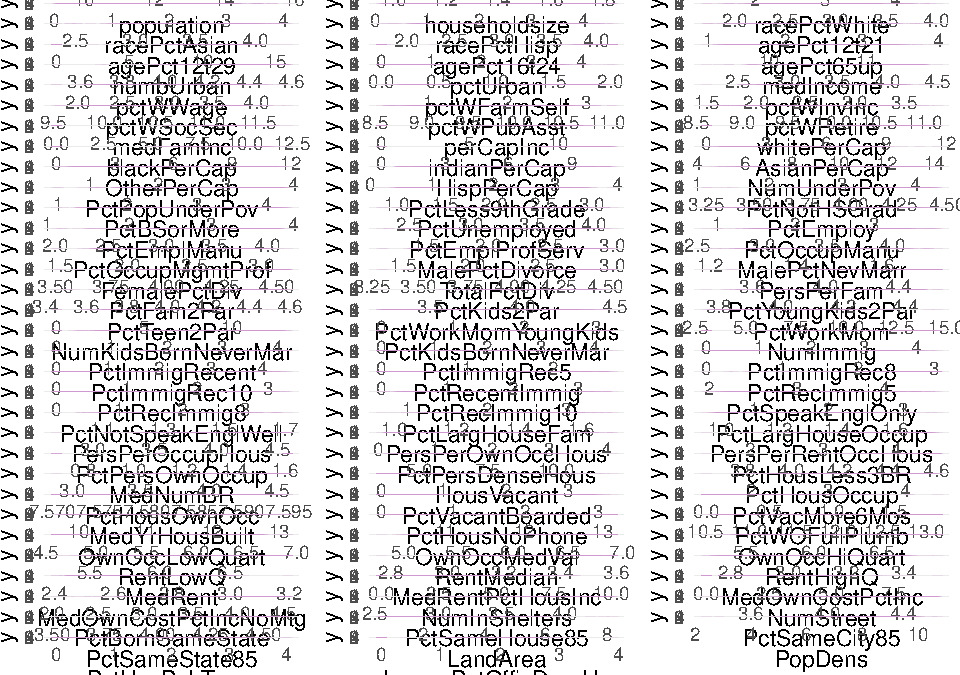
\includegraphics[width=1\linewidth]{dissertation_files/figure-latex/Scatter Plot FULL-1} 

}

\caption{Crime Data. Full Scatter Plot Analysis of Linear Correlations Between Predictors and Target Variable Post Logarithmic Transformation (Over Multiple Pages)}\label{fig:Scatter Plot FULL-1}
\end{figure}
\begin{figure}[H]

{\centering \includegraphics[width=1\linewidth]{dissertation_files/figure-latex/Scatter Plot FULL-2} 

}

\caption{Crime Data. Full Scatter Plot Analysis of Linear Correlations Between Predictors and Target Variable Post Logarithmic Transformation (Over Multiple Pages)}\label{fig:Scatter Plot FULL-2}
\end{figure}
\begin{figure}[H]

{\centering \includegraphics[width=1\linewidth]{dissertation_files/figure-latex/Scatter Plot FULL-3} 

}

\caption{Crime Data. Full Scatter Plot Analysis of Linear Correlations Between Predictors and Target Variable Post Logarithmic Transformation (Over Multiple Pages)}\label{fig:Scatter Plot FULL-3}
\end{figure}
\begin{figure}[H]

{\centering \includegraphics[width=1\linewidth]{dissertation_files/figure-latex/Scatter Plot FULL-4} 

}

\caption{Crime Data. Full Scatter Plot Analysis of Linear Correlations Between Predictors and Target Variable Post Logarithmic Transformation (Over Multiple Pages)}\label{fig:Scatter Plot FULL-4}
\end{figure}
\begin{figure}[H]

{\centering \includegraphics[width=1\linewidth]{dissertation_files/figure-latex/Scatter Plot FULL-5} 

}

\caption{Crime Data. Full Scatter Plot Analysis of Linear Correlations Between Predictors and Target Variable Post Logarithmic Transformation (Over Multiple Pages)}\label{fig:Scatter Plot FULL-5}
\end{figure}

\subsection{Code}

Note that the code should be run from the Analysis Execution part of the
code, while other files should be sourced to run appropriately.

\subsubsection{Data Simulation}

The file should be saved as `simulate\_data.R'.

\begin{Shaded}
\begin{Highlighting}[]
\DocumentationTok{\#\#\#\# SIMULATE T1 UNCORRELATED CONTINUOUS DATA \#\#\#\#}

\CommentTok{\# Function to simulate a T1 type data set}
\CommentTok{\# INPUT: }
\CommentTok{\#       p {-} number of covariates.}
\CommentTok{\#       n {-} number of data points to simulate.}
\CommentTok{\#       sigma\_e {-} variance of the error term.}
\CommentTok{\#       seed {-} seed for random number generation.}
\CommentTok{\#       standardise {-} whether to standardise the variables.}
\CommentTok{\# OUTPUT:}
\CommentTok{\#       sim\_data {-} data frame with simulated data}
\NormalTok{simulate\_T1 }\OtherTok{\textless{}{-}} \ControlFlowTok{function}\NormalTok{(p, n, }\AttributeTok{sigma\_e =} \FunctionTok{sqrt}\NormalTok{(}\DecValTok{15}\NormalTok{), }
                        \AttributeTok{seed =} \DecValTok{42}\NormalTok{, }\AttributeTok{standardise =} \ConstantTok{TRUE}\NormalTok{) \{}
  
  \CommentTok{\# Input validation}
  \ControlFlowTok{if}\NormalTok{ (}\SpecialCharTok{!}\FunctionTok{is.null}\NormalTok{(seed) }\SpecialCharTok{\&\&}\NormalTok{ (}\SpecialCharTok{!}\FunctionTok{is.numeric}\NormalTok{(seed) }\SpecialCharTok{||}\NormalTok{ seed }\SpecialCharTok{\textless{}} \DecValTok{0} \SpecialCharTok{||}\NormalTok{ seed }\SpecialCharTok{\%\%} \DecValTok{1} \SpecialCharTok{!=} \DecValTok{0}\NormalTok{)) \{}
    \CommentTok{\# Check if the seed is a non{-}negative integer.}
    \FunctionTok{stop}\NormalTok{(}\StringTok{"seed must be a non{-}negative integer"}\NormalTok{)}
\NormalTok{  \}}
  
  \ControlFlowTok{if}\NormalTok{ (}\SpecialCharTok{!}\FunctionTok{is.numeric}\NormalTok{(p) }\SpecialCharTok{||}\NormalTok{ p }\SpecialCharTok{\textless{}=} \DecValTok{0} \SpecialCharTok{||} \FunctionTok{floor}\NormalTok{(p) }\SpecialCharTok{!=}\NormalTok{ p) \{}
    \CommentTok{\# Check if p is a positive integer.}
    \FunctionTok{stop}\NormalTok{(}\StringTok{"p must be a positive integer"}\NormalTok{)}
\NormalTok{  \}}
  
  \ControlFlowTok{if}\NormalTok{ (}\SpecialCharTok{!}\FunctionTok{is.numeric}\NormalTok{(n) }\SpecialCharTok{||}\NormalTok{ n }\SpecialCharTok{\textless{}=} \DecValTok{0} \SpecialCharTok{||} \FunctionTok{floor}\NormalTok{(n) }\SpecialCharTok{!=}\NormalTok{ n) \{}
    \CommentTok{\# Check if n is a positive integer.}
    \FunctionTok{stop}\NormalTok{(}\StringTok{"n must be a positive integer"}\NormalTok{)}
\NormalTok{  \}}
  
  \ControlFlowTok{if}\NormalTok{ (}\SpecialCharTok{!}\FunctionTok{is.numeric}\NormalTok{(sigma\_e) }\SpecialCharTok{||}\NormalTok{ sigma\_e }\SpecialCharTok{\textless{}=} \DecValTok{0}\NormalTok{) \{}
    \CommentTok{\# Check if sigma\_e is a positive number.}
    \FunctionTok{stop}\NormalTok{(}\StringTok{"sigma\_e must be a positive number"}\NormalTok{)}
\NormalTok{  \}}
  
  \CommentTok{\# Set seed if not provided}
  \ControlFlowTok{if}\NormalTok{ (}\SpecialCharTok{!}\FunctionTok{is.null}\NormalTok{(seed)) \{}
    \FunctionTok{set.seed}\NormalTok{(seed)}
\NormalTok{  \}}
  
  \CommentTok{\# Set the mean vector}
\NormalTok{  u\_x }\OtherTok{\textless{}{-}} \FunctionTok{rep}\NormalTok{(}\DecValTok{5}\NormalTok{, p)}
  
  \CommentTok{\# Set the correlation matrix as identity matrix}
\NormalTok{  sigma\_x }\OtherTok{\textless{}{-}} \FunctionTok{diag}\NormalTok{(p)}
  
  \CommentTok{\# Generate the covariates X}
\NormalTok{  X }\OtherTok{\textless{}{-}}\NormalTok{ MASS}\SpecialCharTok{::}\FunctionTok{mvrnorm}\NormalTok{(n, }\AttributeTok{mu =}\NormalTok{ u\_x, }\AttributeTok{Sigma =}\NormalTok{ sigma\_x)}
  
  \CommentTok{\# Generate the true regression coefficients beta}
\NormalTok{  beta }\OtherTok{\textless{}{-}} \FunctionTok{c}\NormalTok{(}\FunctionTok{rep}\NormalTok{(}\DecValTok{3}\NormalTok{, }\DecValTok{10}\NormalTok{), }\FunctionTok{rep}\NormalTok{(}\DecValTok{5}\NormalTok{, }\DecValTok{10}\NormalTok{), }\FunctionTok{rep}\NormalTok{(}\DecValTok{0}\NormalTok{, p }\SpecialCharTok{{-}} \DecValTok{20}\NormalTok{))}
  
  \CommentTok{\# Generate the error terms}
\NormalTok{  epsilon }\OtherTok{\textless{}{-}} \FunctionTok{rnorm}\NormalTok{(n, }\AttributeTok{mean =} \DecValTok{0}\NormalTok{, }\AttributeTok{sd =}\NormalTok{ sigma\_e)}
  
  \CommentTok{\# Generate the response variable y}
\NormalTok{  y }\OtherTok{\textless{}{-}}\NormalTok{ X }\SpecialCharTok{\%*\%}\NormalTok{ beta }\SpecialCharTok{+}\NormalTok{ epsilon}
  
  \CommentTok{\# Combine X and y into a data frame}
\NormalTok{  sim\_data }\OtherTok{\textless{}{-}} \FunctionTok{as.data.frame}\NormalTok{(}\FunctionTok{cbind}\NormalTok{(y, X))}
  
  \CommentTok{\# Name the columns of the data frame}
  \FunctionTok{colnames}\NormalTok{(sim\_data) }\OtherTok{\textless{}{-}} \FunctionTok{c}\NormalTok{(}\StringTok{"y"}\NormalTok{, }\FunctionTok{paste0}\NormalTok{(}\StringTok{"X"}\NormalTok{, }\DecValTok{1}\SpecialCharTok{:}\NormalTok{p))}
  
  \ControlFlowTok{if}\NormalTok{ (standardise) \{}
    \CommentTok{\# Standardise only X variables, not y}
\NormalTok{    sim\_data[ , }\SpecialCharTok{{-}}\DecValTok{1}\NormalTok{] }\OtherTok{\textless{}{-}} \FunctionTok{scale}\NormalTok{(sim\_data[ , }\SpecialCharTok{{-}}\DecValTok{1}\NormalTok{])}
\NormalTok{  \}}
  
  \CommentTok{\# Return the dataset}
  \FunctionTok{return}\NormalTok{(sim\_data)}
\NormalTok{\}}

\CommentTok{\# Extract the simulated data}
\CommentTok{\# Simulate where p \textless{} n}
\NormalTok{T1\_LD }\OtherTok{\textless{}{-}} \FunctionTok{simulate\_T1}\NormalTok{(}\AttributeTok{p =} \DecValTok{50}\NormalTok{, }\AttributeTok{n =} \DecValTok{200}\NormalTok{)}
\CommentTok{\# Simulate where p = n}
\NormalTok{T1\_ED }\OtherTok{\textless{}{-}} \FunctionTok{simulate\_T1}\NormalTok{(}\AttributeTok{p =} \DecValTok{100}\NormalTok{, }\AttributeTok{n =} \DecValTok{100}\NormalTok{)}
\CommentTok{\# Simulate where p \textgreater{} n}
\NormalTok{T1\_HD }\OtherTok{\textless{}{-}} \FunctionTok{simulate\_T1}\NormalTok{(}\AttributeTok{p =} \DecValTok{200}\NormalTok{, }\AttributeTok{n =} \DecValTok{150}\NormalTok{)}
\CommentTok{\# Simulate where p \textgreater{}\textgreater{} n}
\NormalTok{T1\_VD }\OtherTok{\textless{}{-}} \FunctionTok{simulate\_T1}\NormalTok{(}\AttributeTok{p =} \DecValTok{200}\NormalTok{, }\AttributeTok{n =} \DecValTok{50}\NormalTok{)}
\CommentTok{\# Simulate for XGBoost p \textless{}\textless{} n}
\NormalTok{T1\_XD }\OtherTok{\textless{}{-}} \FunctionTok{simulate\_T1}\NormalTok{(}\AttributeTok{p =} \DecValTok{50}\NormalTok{, }\AttributeTok{n =} \DecValTok{500}\NormalTok{)}

\DocumentationTok{\#\#\#\# SIMULATE T2 TEMPORAL CORRELATED CONTINUOUS DATA \#\#\#\#}

\CommentTok{\# Function to simulate a T2 type data set}
\CommentTok{\# INPUT: }
\CommentTok{\#       p {-} number of covariates}
\CommentTok{\#       n {-} number of data points to simulate}
\CommentTok{\#       rho {-} AR(1) correlation coefficient}
\CommentTok{\#       sigma\_e {-} variance of the error term}
\CommentTok{\#       seed {-} seed for random number generation}
\CommentTok{\#       standardise {-} whether to standardise the variables.}
\CommentTok{\# OUTPUT:}
\CommentTok{\#       sim\_data {-} data frame with simulated data}
\NormalTok{simulate\_T2 }\OtherTok{\textless{}{-}} \ControlFlowTok{function}\NormalTok{(p, n, }\AttributeTok{rho =} \FloatTok{0.8}\NormalTok{, }\AttributeTok{sigma\_e =} \FunctionTok{sqrt}\NormalTok{(}\DecValTok{10}\NormalTok{), }
                        \AttributeTok{seed =} \DecValTok{42}\NormalTok{, }\AttributeTok{standardise =} \ConstantTok{TRUE}\NormalTok{) \{}
  
  \CommentTok{\# Input validation}
  \ControlFlowTok{if}\NormalTok{ (}\SpecialCharTok{!}\FunctionTok{is.null}\NormalTok{(seed) }\SpecialCharTok{\&\&}\NormalTok{ (}\SpecialCharTok{!}\FunctionTok{is.numeric}\NormalTok{(seed) }\SpecialCharTok{||}\NormalTok{ seed }\SpecialCharTok{\textless{}} \DecValTok{0} \SpecialCharTok{||}\NormalTok{ seed }\SpecialCharTok{\%\%} \DecValTok{1} \SpecialCharTok{!=} \DecValTok{0}\NormalTok{)) \{}
    \CommentTok{\# Check if the seed is a non{-}negative integer.}
    \FunctionTok{stop}\NormalTok{(}\StringTok{"seed must be a non{-}negative integer"}\NormalTok{)}
\NormalTok{  \}}
  
  \ControlFlowTok{if}\NormalTok{ (}\SpecialCharTok{!}\FunctionTok{is.numeric}\NormalTok{(p) }\SpecialCharTok{||}\NormalTok{ p }\SpecialCharTok{\textless{}=} \DecValTok{0} \SpecialCharTok{||} \FunctionTok{floor}\NormalTok{(p) }\SpecialCharTok{!=}\NormalTok{ p) \{}
    \CommentTok{\# Check if p is a positive integer.}
    \FunctionTok{stop}\NormalTok{(}\StringTok{"p must be a positive integer"}\NormalTok{)}
\NormalTok{  \}}
  
  \ControlFlowTok{if}\NormalTok{ (}\SpecialCharTok{!}\FunctionTok{is.numeric}\NormalTok{(n) }\SpecialCharTok{||}\NormalTok{ n }\SpecialCharTok{\textless{}=} \DecValTok{0} \SpecialCharTok{||} \FunctionTok{floor}\NormalTok{(n) }\SpecialCharTok{!=}\NormalTok{ n) \{}
    \CommentTok{\# Check if n is a positive integer.}
    \FunctionTok{stop}\NormalTok{(}\StringTok{"n must be a positive integer"}\NormalTok{)}
\NormalTok{  \}}
  
  \ControlFlowTok{if}\NormalTok{ (}\SpecialCharTok{!}\FunctionTok{is.numeric}\NormalTok{(sigma\_e) }\SpecialCharTok{||}\NormalTok{ sigma\_e }\SpecialCharTok{\textless{}=} \DecValTok{0}\NormalTok{) \{}
    \CommentTok{\# Check if sigma\_e is a positive number.}
    \FunctionTok{stop}\NormalTok{(}\StringTok{"sigma\_e must be a positive number"}\NormalTok{)}
\NormalTok{  \}}
  
  \ControlFlowTok{if}\NormalTok{ (}\SpecialCharTok{!}\FunctionTok{is.numeric}\NormalTok{(rho) }\SpecialCharTok{||}\NormalTok{ rho }\SpecialCharTok{\textless{}} \SpecialCharTok{{-}}\DecValTok{1} \SpecialCharTok{||}\NormalTok{ rho }\SpecialCharTok{\textgreater{}} \DecValTok{1}\NormalTok{) \{}
    \CommentTok{\# Check if rho is a number between {-}1 and 1.}
    \FunctionTok{stop}\NormalTok{(}\StringTok{"rho must be a number between {-}1 and 1"}\NormalTok{)}
\NormalTok{  \}}
  
  \CommentTok{\# Set seed if not provided}
  \ControlFlowTok{if}\NormalTok{ (}\SpecialCharTok{!}\FunctionTok{is.null}\NormalTok{(seed)) \{}
    \FunctionTok{set.seed}\NormalTok{(seed)}
\NormalTok{  \}}
  
  \CommentTok{\# Set the mean vector}
\NormalTok{  u\_x }\OtherTok{\textless{}{-}} \FunctionTok{c}\NormalTok{(}\FunctionTok{rep}\NormalTok{(}\DecValTok{3}\NormalTok{, }\DecValTok{30}\NormalTok{), }\FunctionTok{rep}\NormalTok{(}\DecValTok{7}\NormalTok{, p}\DecValTok{{-}30}\NormalTok{))}
  
  \CommentTok{\# Set the covariance matrix with AR(1) structure}
\NormalTok{  sigma\_x }\OtherTok{\textless{}{-}} \FunctionTok{matrix}\NormalTok{(rho}\SpecialCharTok{\^{}}\FunctionTok{abs}\NormalTok{(}\FunctionTok{outer}\NormalTok{(}\DecValTok{1}\SpecialCharTok{:}\NormalTok{p, }\DecValTok{1}\SpecialCharTok{:}\NormalTok{p, }\StringTok{"{-}"}\NormalTok{)), p, p)}
  
  \CommentTok{\# Generate the covariates X}
\NormalTok{  X }\OtherTok{\textless{}{-}}\NormalTok{ MASS}\SpecialCharTok{::}\FunctionTok{mvrnorm}\NormalTok{(n, }\AttributeTok{mu =}\NormalTok{ u\_x, }\AttributeTok{Sigma =}\NormalTok{ sigma\_x)}
  
  \CommentTok{\# Generate the true regression coefficients beta}
\NormalTok{  beta }\OtherTok{\textless{}{-}} \FunctionTok{c}\NormalTok{(}\FunctionTok{seq}\NormalTok{(}\DecValTok{1}\NormalTok{, }\DecValTok{20}\NormalTok{, }\DecValTok{1}\NormalTok{), }\FunctionTok{rep}\NormalTok{(}\DecValTok{0}\NormalTok{, p }\SpecialCharTok{{-}} \DecValTok{20}\NormalTok{))}
  
  \CommentTok{\# Generate the error terms}
\NormalTok{  epsilon }\OtherTok{\textless{}{-}} \FunctionTok{rnorm}\NormalTok{(n, }\AttributeTok{mean =} \DecValTok{0}\NormalTok{, }\AttributeTok{sd =}\NormalTok{ sigma\_e)}
  
  \CommentTok{\# Generate the response variable y}
\NormalTok{  y }\OtherTok{\textless{}{-}}\NormalTok{ X }\SpecialCharTok{\%*\%}\NormalTok{ beta }\SpecialCharTok{+}\NormalTok{ epsilon}
  
  \CommentTok{\# Combine X and y into a data frame}
\NormalTok{  sim\_data }\OtherTok{\textless{}{-}} \FunctionTok{as.data.frame}\NormalTok{(}\FunctionTok{cbind}\NormalTok{(y, X))}
  
  \CommentTok{\# Name the columns of the data frame}
  \FunctionTok{colnames}\NormalTok{(sim\_data) }\OtherTok{\textless{}{-}} \FunctionTok{c}\NormalTok{(}\StringTok{"y"}\NormalTok{, }\FunctionTok{paste0}\NormalTok{(}\StringTok{"X"}\NormalTok{, }\DecValTok{1}\SpecialCharTok{:}\NormalTok{p))}
  
  \ControlFlowTok{if}\NormalTok{ (standardise) \{}
    \CommentTok{\# Standardise only X variables, not y}
\NormalTok{    sim\_data[ , }\SpecialCharTok{{-}}\DecValTok{1}\NormalTok{] }\OtherTok{\textless{}{-}} \FunctionTok{scale}\NormalTok{(sim\_data[ , }\SpecialCharTok{{-}}\DecValTok{1}\NormalTok{])}
\NormalTok{  \}}
  
  \CommentTok{\# Return the dataset}
  \FunctionTok{return}\NormalTok{(sim\_data)}
\NormalTok{\}}

\CommentTok{\# Simulate where p \textless{} n}
\NormalTok{T2\_LD }\OtherTok{\textless{}{-}} \FunctionTok{simulate\_T2}\NormalTok{(}\AttributeTok{p =} \DecValTok{50}\NormalTok{, }\AttributeTok{n =} \DecValTok{200}\NormalTok{)}
\CommentTok{\# Simulate where p = n}
\NormalTok{T2\_ED }\OtherTok{\textless{}{-}} \FunctionTok{simulate\_T2}\NormalTok{(}\AttributeTok{p =} \DecValTok{100}\NormalTok{, }\AttributeTok{n =} \DecValTok{100}\NormalTok{)}
\CommentTok{\# Simulate where p \textgreater{} n}
\NormalTok{T2\_HD }\OtherTok{\textless{}{-}} \FunctionTok{simulate\_T2}\NormalTok{(}\AttributeTok{p =} \DecValTok{200}\NormalTok{, }\AttributeTok{n =} \DecValTok{150}\NormalTok{)}
\CommentTok{\# Simulate where p \textgreater{}\textgreater{} n}
\NormalTok{T2\_VD }\OtherTok{\textless{}{-}} \FunctionTok{simulate\_T2}\NormalTok{(}\AttributeTok{p =} \DecValTok{200}\NormalTok{, }\AttributeTok{n =} \DecValTok{50}\NormalTok{)}
\CommentTok{\# Simulate for XGBoost p \textless{}\textless{} n}
\NormalTok{T2\_XD }\OtherTok{\textless{}{-}} \FunctionTok{simulate\_T2}\NormalTok{(}\AttributeTok{p =} \DecValTok{50}\NormalTok{, }\AttributeTok{n =} \DecValTok{500}\NormalTok{)}

\DocumentationTok{\#\#\#\# SIMULATE T3 MIXED CONTINUOUS AND CATEGORICAL DATA \#\#\#\#}

\CommentTok{\# Function to simulate a T3 type data set with mixed continuous and }
\CommentTok{\#     categorical variables, and some polynomials, interaction terms.}
\CommentTok{\# INPUT: }
\CommentTok{\#       p {-} number of continuous covariates (minimum of 10).}
\CommentTok{\#       n {-} number of data points to simulate.}
\CommentTok{\#       rho {-} AR(1) correlation coefficient.}
\CommentTok{\#       sigma\_e {-} variance of the error term.}
\CommentTok{\#       seed {-} seed for random number generation.}
\CommentTok{\#       standardise {-} whether to standardise the variables.}
\CommentTok{\# OUTPUT:}
\CommentTok{\#       sim\_data {-} data frame with simulated data}
\NormalTok{simulate\_T3 }\OtherTok{\textless{}{-}} \ControlFlowTok{function}\NormalTok{(p, n, }\AttributeTok{rho =} \FloatTok{0.6}\NormalTok{, }\AttributeTok{sigma\_e =} \FunctionTok{sqrt}\NormalTok{(}\DecValTok{12}\NormalTok{), }
                        \AttributeTok{seed =} \DecValTok{42}\NormalTok{, }\AttributeTok{standardise =} \ConstantTok{TRUE}\NormalTok{) \{}
  
  \CommentTok{\# Input validation}
  \ControlFlowTok{if}\NormalTok{ (}\SpecialCharTok{!}\FunctionTok{is.null}\NormalTok{(seed) }\SpecialCharTok{\&\&}\NormalTok{ (}\SpecialCharTok{!}\FunctionTok{is.numeric}\NormalTok{(seed) }\SpecialCharTok{||}\NormalTok{ seed }\SpecialCharTok{\textless{}} \DecValTok{0} \SpecialCharTok{||}\NormalTok{ seed }\SpecialCharTok{\%\%} \DecValTok{1} \SpecialCharTok{!=} \DecValTok{0}\NormalTok{)) \{}
    \CommentTok{\# Check if the seed is a non{-}negative integer.}
    \FunctionTok{stop}\NormalTok{(}\StringTok{"seed must be a non{-}negative integer"}\NormalTok{)}
\NormalTok{  \}}
  
  \ControlFlowTok{if}\NormalTok{ (}\SpecialCharTok{!}\FunctionTok{is.numeric}\NormalTok{(p) }\SpecialCharTok{||}\NormalTok{ p }\SpecialCharTok{\textless{}=} \DecValTok{0} \SpecialCharTok{||} \FunctionTok{floor}\NormalTok{(p) }\SpecialCharTok{!=}\NormalTok{ p) \{}
    \CommentTok{\# Check if p is a positive integer.}
    \FunctionTok{stop}\NormalTok{(}\StringTok{"p must be a positive integer"}\NormalTok{)}
\NormalTok{  \}}
  
  \ControlFlowTok{if}\NormalTok{ (}\SpecialCharTok{!}\FunctionTok{is.numeric}\NormalTok{(n) }\SpecialCharTok{||}\NormalTok{ n }\SpecialCharTok{\textless{}=} \DecValTok{0} \SpecialCharTok{||} \FunctionTok{floor}\NormalTok{(n) }\SpecialCharTok{!=}\NormalTok{ n) \{}
    \CommentTok{\# Check if n is a positive integer.}
    \FunctionTok{stop}\NormalTok{(}\StringTok{"n must be a positive integer"}\NormalTok{)}
\NormalTok{  \}}
  
  \ControlFlowTok{if}\NormalTok{ (}\SpecialCharTok{!}\FunctionTok{is.numeric}\NormalTok{(sigma\_e) }\SpecialCharTok{||}\NormalTok{ sigma\_e }\SpecialCharTok{\textless{}=} \DecValTok{0}\NormalTok{) \{}
    \CommentTok{\# Check if sigma\_e is a positive number.}
    \FunctionTok{stop}\NormalTok{(}\StringTok{"sigma\_e must be a positive number"}\NormalTok{)}
\NormalTok{  \}}
  
  \ControlFlowTok{if}\NormalTok{ (}\SpecialCharTok{!}\FunctionTok{is.numeric}\NormalTok{(rho) }\SpecialCharTok{||}\NormalTok{ rho }\SpecialCharTok{\textless{}} \SpecialCharTok{{-}}\DecValTok{1} \SpecialCharTok{||}\NormalTok{ rho }\SpecialCharTok{\textgreater{}} \DecValTok{1}\NormalTok{) \{}
    \CommentTok{\# Check if rho is a number between {-}1 and 1.}
    \FunctionTok{stop}\NormalTok{(}\StringTok{"rho must be a number between {-}1 and 1"}\NormalTok{)}
\NormalTok{  \}}
  
  \CommentTok{\# Set seed if not provided}
  \ControlFlowTok{if}\NormalTok{ (}\SpecialCharTok{!}\FunctionTok{is.null}\NormalTok{(seed)) \{}
    \FunctionTok{set.seed}\NormalTok{(seed)}
\NormalTok{  \}}
  
  \CommentTok{\# Calculate the number of continuous covariates needed}
  \CommentTok{\# 10 for 2 categorical, 4 interactions, and 4 polynomials}
\NormalTok{  p }\OtherTok{\textless{}{-}}\NormalTok{ p }\SpecialCharTok{{-}} \DecValTok{10}  
  
  \CommentTok{\# Set the mean vector for continuous covariates}
\NormalTok{  u\_x }\OtherTok{\textless{}{-}} \FunctionTok{c}\NormalTok{(}\FunctionTok{rep}\NormalTok{(}\DecValTok{2}\NormalTok{, }\DecValTok{10}\NormalTok{), }\FunctionTok{rep}\NormalTok{(}\DecValTok{5}\NormalTok{, }\DecValTok{30}\NormalTok{), }\FunctionTok{rep}\NormalTok{(}\DecValTok{8}\NormalTok{, p }\SpecialCharTok{{-}} \DecValTok{40}\NormalTok{))}
  
  \CommentTok{\# Set the covariance matrix with AR(1) structure}
\NormalTok{  sigma\_x }\OtherTok{\textless{}{-}} \FunctionTok{matrix}\NormalTok{(rho}\SpecialCharTok{\^{}}\FunctionTok{abs}\NormalTok{(}\FunctionTok{outer}\NormalTok{(}\DecValTok{1}\SpecialCharTok{:}\NormalTok{p, }\DecValTok{1}\SpecialCharTok{:}\NormalTok{p, }\StringTok{"{-}"}\NormalTok{)), p, p)}
  
  \CommentTok{\# Generate the continuous covariates X}
\NormalTok{  X }\OtherTok{\textless{}{-}}\NormalTok{ MASS}\SpecialCharTok{::}\FunctionTok{mvrnorm}\NormalTok{(n, }\AttributeTok{mu =}\NormalTok{ u\_x, }\AttributeTok{Sigma =}\NormalTok{ sigma\_x)}
  
  \CommentTok{\# Generate binary categorical variable}
\NormalTok{  cat\_var1 }\OtherTok{\textless{}{-}} \FunctionTok{sample}\NormalTok{(}\FunctionTok{c}\NormalTok{(}\DecValTok{0}\NormalTok{, }\DecValTok{1}\NormalTok{), n, }\AttributeTok{replace =} \ConstantTok{TRUE}\NormalTok{) }\SpecialCharTok{\%\textgreater{}\%} 
    \FunctionTok{as.factor}\NormalTok{()}
  \CommentTok{\# Treat as ordinal categorical variable}
\NormalTok{  cat\_var2 }\OtherTok{\textless{}{-}} \FunctionTok{sample}\NormalTok{(}\DecValTok{1}\SpecialCharTok{:}\DecValTok{5}\NormalTok{, n, }\AttributeTok{replace =} \ConstantTok{TRUE}\NormalTok{) }\SpecialCharTok{\%\textgreater{}\%} 
    \FunctionTok{as.factor}\NormalTok{()}
  
  \CommentTok{\# Generate interaction terms (multiplying first and second continuous covariate)}
\NormalTok{  interaction\_term\_1\_2 }\OtherTok{\textless{}{-}}\NormalTok{ X[, }\DecValTok{1}\NormalTok{] }\SpecialCharTok{*}\NormalTok{ X[, }\DecValTok{2}\NormalTok{]}
\NormalTok{  interaction\_term\_3\_4 }\OtherTok{\textless{}{-}}\NormalTok{ X[, }\DecValTok{3}\NormalTok{] }\SpecialCharTok{*}\NormalTok{ X[, }\DecValTok{4}\NormalTok{]}
\NormalTok{  interaction\_term\_21\_22 }\OtherTok{\textless{}{-}}\NormalTok{ X[, }\DecValTok{21}\NormalTok{] }\SpecialCharTok{*}\NormalTok{ X[, }\DecValTok{22}\NormalTok{]}
\NormalTok{  interaction\_term\_c1\_22 }\OtherTok{\textless{}{-}} \FunctionTok{interaction}\NormalTok{(cat\_var1, X[, }\DecValTok{22}\NormalTok{])}
  
  \CommentTok{\# Generate polynomial feature (squared third continuous covariate)}
\NormalTok{  polynomial\_feature\_5\_2 }\OtherTok{\textless{}{-}}\NormalTok{ X[, }\DecValTok{5}\NormalTok{]}\SpecialCharTok{\^{}}\DecValTok{2}
\NormalTok{  polynomial\_feature\_6\_3 }\OtherTok{\textless{}{-}}\NormalTok{ X[, }\DecValTok{6}\NormalTok{]}\SpecialCharTok{\^{}}\DecValTok{3}
\NormalTok{  polynomial\_feature\_23\_2 }\OtherTok{\textless{}{-}}\NormalTok{ X[, }\DecValTok{23}\NormalTok{]}\SpecialCharTok{\^{}}\DecValTok{2}
\NormalTok{  polynomial\_feature\_23\_3 }\OtherTok{\textless{}{-}}\NormalTok{ X[, }\DecValTok{23}\NormalTok{]}\SpecialCharTok{\^{}}\DecValTok{3}
  
  \CommentTok{\# Generate the true regression coefficients beta}
\NormalTok{  beta }\OtherTok{\textless{}{-}} \FunctionTok{c}\NormalTok{(}\FunctionTok{rep}\NormalTok{(}\DecValTok{6}\NormalTok{, }\DecValTok{5}\NormalTok{), }\FunctionTok{rep}\NormalTok{(}\DecValTok{4}\NormalTok{, }\DecValTok{5}\NormalTok{), }\FunctionTok{rep}\NormalTok{(}\DecValTok{3}\NormalTok{, }\DecValTok{5}\NormalTok{), }\FunctionTok{rep}\NormalTok{(}\DecValTok{0}\NormalTok{, p }\SpecialCharTok{{-}} \DecValTok{15}\NormalTok{))}
  
  \CommentTok{\# Generate the error terms}
\NormalTok{  epsilon }\OtherTok{\textless{}{-}} \FunctionTok{rnorm}\NormalTok{(n, }\AttributeTok{mean =} \DecValTok{0}\NormalTok{, }\AttributeTok{sd =}\NormalTok{ sigma\_e)}
  
  \CommentTok{\# Add the intercept too}
\NormalTok{  intercept }\OtherTok{\textless{}{-}} \DecValTok{2}
  
  \CommentTok{\# Define the betas}
\NormalTok{  beta\_cat\_var1 }\OtherTok{\textless{}{-}} \DecValTok{4}
\NormalTok{  beta\_it\_1\_2 }\OtherTok{\textless{}{-}} \DecValTok{3}
\NormalTok{  beta\_p\_23\_2 }\OtherTok{\textless{}{-}} \DecValTok{6}
  
  \CommentTok{\# Use zero for all other betas}
\NormalTok{  beta\_cat\_var2 }\OtherTok{\textless{}{-}} \DecValTok{0}
\NormalTok{  beta\_it\_3\_4 }\OtherTok{\textless{}{-}} \DecValTok{0}
\NormalTok{  beta\_it\_21\_22 }\OtherTok{\textless{}{-}} \DecValTok{0}
\NormalTok{  beta\_it\_c1\_22 }\OtherTok{\textless{}{-}} \DecValTok{0}
\NormalTok{  beta\_p\_5 }\OtherTok{\textless{}{-}} \DecValTok{0}
\NormalTok{  beta\_p\_6 }\OtherTok{\textless{}{-}} \DecValTok{0}
\NormalTok{  beta\_p\_23\_3 }\OtherTok{\textless{}{-}} \DecValTok{0}
  
  \CommentTok{\# Generate the response variable y}
\NormalTok{  y }\OtherTok{\textless{}{-}}\NormalTok{ intercept }\SpecialCharTok{+}\NormalTok{ X }\SpecialCharTok{\%*\%}\NormalTok{ beta }\SpecialCharTok{+} 
\NormalTok{    beta\_cat\_var1 }\SpecialCharTok{*} \FunctionTok{as.numeric}\NormalTok{(cat\_var1) }\SpecialCharTok{+} 
\NormalTok{    beta\_cat\_var2 }\SpecialCharTok{*} \FunctionTok{as.numeric}\NormalTok{(cat\_var2) }\SpecialCharTok{+} 
\NormalTok{    beta\_it\_1\_2 }\SpecialCharTok{*}\NormalTok{ interaction\_term\_1\_2 }\SpecialCharTok{+} 
\NormalTok{    beta\_it\_3\_4 }\SpecialCharTok{*}\NormalTok{ interaction\_term\_3\_4 }\SpecialCharTok{+} 
\NormalTok{    beta\_it\_21\_22 }\SpecialCharTok{*}\NormalTok{ interaction\_term\_21\_22 }\SpecialCharTok{+} 
\NormalTok{    beta\_it\_c1\_22 }\SpecialCharTok{*} \FunctionTok{as.numeric}\NormalTok{(interaction\_term\_c1\_22) }\SpecialCharTok{+}
\NormalTok{    beta\_p\_5 }\SpecialCharTok{*}\NormalTok{ polynomial\_feature\_5\_2 }\SpecialCharTok{+} 
\NormalTok{    beta\_p\_6 }\SpecialCharTok{*}\NormalTok{ polynomial\_feature\_6\_3 }\SpecialCharTok{+} 
\NormalTok{    beta\_p\_23\_2 }\SpecialCharTok{*}\NormalTok{ polynomial\_feature\_23\_2 }\SpecialCharTok{+}
\NormalTok{    beta\_p\_23\_3 }\SpecialCharTok{*}\NormalTok{ polynomial\_feature\_23\_3 }\SpecialCharTok{+}
\NormalTok{    epsilon}
  
  \CommentTok{\# Combine continuous covariates, categorical vars, interaction terms, }
  \CommentTok{\# polynomial features and y into a data frame}
\NormalTok{  sim\_data }\OtherTok{\textless{}{-}} \FunctionTok{as.data.frame}\NormalTok{(}\FunctionTok{cbind}\NormalTok{(y, }
\NormalTok{                                  cat\_var1, }
\NormalTok{                                  cat\_var2, }
\NormalTok{                                  interaction\_term\_1\_2, }
\NormalTok{                                  interaction\_term\_3\_4,}
\NormalTok{                                  interaction\_term\_21\_22,}
\NormalTok{                                  interaction\_term\_c1\_22,}
\NormalTok{                                  polynomial\_feature\_5\_2,}
\NormalTok{                                  polynomial\_feature\_6\_3, }
\NormalTok{                                  polynomial\_feature\_23\_2,}
\NormalTok{                                  polynomial\_feature\_23\_3, X))}
  
  \CommentTok{\# Make sure the categorical variables are factors}
\NormalTok{  sim\_data}\SpecialCharTok{$}\NormalTok{cat\_var1 }\OtherTok{\textless{}{-}} \FunctionTok{as.factor}\NormalTok{(sim\_data}\SpecialCharTok{$}\NormalTok{cat\_var1)}
\NormalTok{  sim\_data}\SpecialCharTok{$}\NormalTok{cat\_var2 }\OtherTok{\textless{}{-}} \FunctionTok{as.factor}\NormalTok{(sim\_data}\SpecialCharTok{$}\NormalTok{cat\_var2)}
  
  \CommentTok{\# Name the columns of the data frame}
  \FunctionTok{colnames}\NormalTok{(sim\_data) }\OtherTok{\textless{}{-}} \FunctionTok{c}\NormalTok{(}\StringTok{"y"}\NormalTok{, }\StringTok{"cat\_var1"}\NormalTok{, }\StringTok{"cat\_var2"}\NormalTok{, }
                          \StringTok{"interaction\_1\_2"}\NormalTok{, }\StringTok{"interaction\_3\_4"}\NormalTok{,}
                          \StringTok{"interaction\_21\_22"}\NormalTok{, }\StringTok{"interaction\_term\_c1\_22"}\NormalTok{, }
                          \StringTok{"poly\_5\_2"}\NormalTok{, }\StringTok{"poly\_6\_3"}\NormalTok{, }\StringTok{"poly\_23\_2"}\NormalTok{, }\StringTok{"poly\_23\_3"}\NormalTok{,}
                          \FunctionTok{paste0}\NormalTok{(}\StringTok{"X"}\NormalTok{, }\DecValTok{1}\SpecialCharTok{:}\NormalTok{p))}
  
  \ControlFlowTok{if}\NormalTok{ (standardise) \{}
    \CommentTok{\# Select all variables except y, cat\_var1, cat\_var2}
\NormalTok{    variables\_to\_scale }\OtherTok{\textless{}{-}} \FunctionTok{setdiff}\NormalTok{(}\FunctionTok{colnames}\NormalTok{(sim\_data), }\FunctionTok{c}\NormalTok{(}\StringTok{"y"}\NormalTok{, }\StringTok{"cat\_var1"}\NormalTok{, }\StringTok{"cat\_var2"}\NormalTok{))}
    
    \CommentTok{\# Apply scale() to these variables}
\NormalTok{    sim\_data[variables\_to\_scale] }\OtherTok{\textless{}{-}} \FunctionTok{scale}\NormalTok{(sim\_data[variables\_to\_scale])}
\NormalTok{  \}}
  
  \CommentTok{\# Return the dataset}
  \FunctionTok{return}\NormalTok{(sim\_data)}
\NormalTok{\}}

\CommentTok{\# Simulate where p \textless{} n}
\NormalTok{T3\_LD }\OtherTok{\textless{}{-}} \FunctionTok{simulate\_T3}\NormalTok{(}\AttributeTok{p =} \DecValTok{50}\NormalTok{, }\AttributeTok{n =} \DecValTok{200}\NormalTok{)}
\CommentTok{\# Simulate where p = n}
\NormalTok{T3\_ED }\OtherTok{\textless{}{-}} \FunctionTok{simulate\_T3}\NormalTok{(}\AttributeTok{p =} \DecValTok{100}\NormalTok{, }\AttributeTok{n =} \DecValTok{100}\NormalTok{)}
\CommentTok{\# Simulate where p \textgreater{} n}
\NormalTok{T3\_HD }\OtherTok{\textless{}{-}} \FunctionTok{simulate\_T3}\NormalTok{(}\AttributeTok{p =} \DecValTok{200}\NormalTok{, }\AttributeTok{n =} \DecValTok{150}\NormalTok{)}
\CommentTok{\# Simulate where p \textgreater{}\textgreater{} n}
\NormalTok{T3\_VD }\OtherTok{\textless{}{-}} \FunctionTok{simulate\_T3}\NormalTok{(}\AttributeTok{p =} \DecValTok{200}\NormalTok{, }\AttributeTok{n =} \DecValTok{50}\NormalTok{)}
\CommentTok{\# Simulate for XGBoost p \textless{}\textless{} n}
\NormalTok{T3\_XD }\OtherTok{\textless{}{-}} \FunctionTok{simulate\_T3}\NormalTok{(}\AttributeTok{p =} \DecValTok{50}\NormalTok{, }\AttributeTok{n =} \DecValTok{500}\NormalTok{)}

\DocumentationTok{\#\#\#\# SIMULATE T4 GROUPED CONTINUOUS DATA WITH CATEGORICAL VARIABLES AND INTERACTIONS \#\#\#\#}

\CommentTok{\# Function to simulate a T4 type data set}
\CommentTok{\# INPUT: }
\CommentTok{\#       p {-} number of continuous covariates.}
\CommentTok{\#       n {-} number of data points to simulate.}
\CommentTok{\#       rho {-} within{-}group correlation coefficient.}
\CommentTok{\#       sigma\_e {-} variance of the error term.}
\CommentTok{\#       seed {-} seed for random number generation.}
\CommentTok{\#       standardise {-} whether to standardise the variables.}
\CommentTok{\# OUTPUT:}
\CommentTok{\#       sim\_data {-} data frame with simulated data}
\NormalTok{simulate\_T4 }\OtherTok{\textless{}{-}} \ControlFlowTok{function}\NormalTok{(p, n, }\AttributeTok{rho =} \FloatTok{0.6}\NormalTok{, }\AttributeTok{sigma\_e =} \FunctionTok{sqrt}\NormalTok{(}\DecValTok{10}\NormalTok{), }
                        \AttributeTok{seed =} \DecValTok{42}\NormalTok{, }\AttributeTok{standardise =} \ConstantTok{TRUE}\NormalTok{) \{}
  
  \CommentTok{\# Input validation}
  \ControlFlowTok{if}\NormalTok{ (}\SpecialCharTok{!}\FunctionTok{is.null}\NormalTok{(seed) }\SpecialCharTok{\&\&}\NormalTok{ (}\SpecialCharTok{!}\FunctionTok{is.numeric}\NormalTok{(seed) }\SpecialCharTok{||}\NormalTok{ seed }\SpecialCharTok{\textless{}} \DecValTok{0} \SpecialCharTok{||}\NormalTok{ seed }\SpecialCharTok{\%\%} \DecValTok{1} \SpecialCharTok{!=} \DecValTok{0}\NormalTok{)) \{}
    \CommentTok{\# Check if the seed is a non{-}negative integer.}
    \FunctionTok{stop}\NormalTok{(}\StringTok{"seed must be a non{-}negative integer"}\NormalTok{)}
\NormalTok{  \}}
  
  \ControlFlowTok{if}\NormalTok{ (}\SpecialCharTok{!}\FunctionTok{is.numeric}\NormalTok{(p) }\SpecialCharTok{||}\NormalTok{ p }\SpecialCharTok{\textless{}=} \DecValTok{0} \SpecialCharTok{||} \FunctionTok{floor}\NormalTok{(p) }\SpecialCharTok{!=}\NormalTok{ p) \{}
    \CommentTok{\# Check if p is a positive integer.}
    \FunctionTok{stop}\NormalTok{(}\StringTok{"p must be a positive integer"}\NormalTok{)}
\NormalTok{  \}}
  
  \ControlFlowTok{if}\NormalTok{ (}\SpecialCharTok{!}\FunctionTok{is.numeric}\NormalTok{(n) }\SpecialCharTok{||}\NormalTok{ n }\SpecialCharTok{\textless{}=} \DecValTok{0} \SpecialCharTok{||} \FunctionTok{floor}\NormalTok{(n) }\SpecialCharTok{!=}\NormalTok{ n) \{}
    \CommentTok{\# Check if n is a positive integer.}
    \FunctionTok{stop}\NormalTok{(}\StringTok{"n must be a positive integer"}\NormalTok{)}
\NormalTok{  \}}
  
  \ControlFlowTok{if}\NormalTok{ (}\SpecialCharTok{!}\FunctionTok{is.numeric}\NormalTok{(sigma\_e) }\SpecialCharTok{||}\NormalTok{ sigma\_e }\SpecialCharTok{\textless{}=} \DecValTok{0}\NormalTok{) \{}
    \CommentTok{\# Check if sigma\_e is a positive number.}
    \FunctionTok{stop}\NormalTok{(}\StringTok{"sigma\_e must be a positive number"}\NormalTok{)}
\NormalTok{  \}}
  
  \ControlFlowTok{if}\NormalTok{ (}\SpecialCharTok{!}\FunctionTok{is.numeric}\NormalTok{(rho) }\SpecialCharTok{||}\NormalTok{ rho }\SpecialCharTok{\textless{}} \SpecialCharTok{{-}}\DecValTok{1} \SpecialCharTok{||}\NormalTok{ rho }\SpecialCharTok{\textgreater{}} \DecValTok{1}\NormalTok{) \{}
    \CommentTok{\# Check if rho is a number between {-}1 and 1.}
    \FunctionTok{stop}\NormalTok{(}\StringTok{"rho must be a number between {-}1 and 1"}\NormalTok{)}
\NormalTok{  \}}
  
  \CommentTok{\# Set seed if not provided}
  \ControlFlowTok{if}\NormalTok{ (}\SpecialCharTok{!}\FunctionTok{is.null}\NormalTok{(seed)) \{}
    \FunctionTok{set.seed}\NormalTok{(seed)}
\NormalTok{  \}}
  
  \CommentTok{\# Adjust p to generate the correct number of continuous variables}
\NormalTok{  p }\OtherTok{\textless{}{-}}\NormalTok{ p }\SpecialCharTok{{-}} \DecValTok{5}
  
  \CommentTok{\# Group sizes}
\NormalTok{  group\_sizes }\OtherTok{\textless{}{-}} \FunctionTok{rep}\NormalTok{(p }\SpecialCharTok{/} \DecValTok{5}\NormalTok{, }\DecValTok{5}\NormalTok{)}
  
  \CommentTok{\# Covariance matrices for each group}
\NormalTok{  cov\_matrices }\OtherTok{\textless{}{-}} \FunctionTok{lapply}\NormalTok{(}\DecValTok{1}\SpecialCharTok{:}\DecValTok{5}\NormalTok{, }\ControlFlowTok{function}\NormalTok{(i) \{}
    \FunctionTok{matrix}\NormalTok{(rho, }\AttributeTok{nrow =}\NormalTok{ group\_sizes[i], }\AttributeTok{ncol =}\NormalTok{ group\_sizes[i]) }\SpecialCharTok{+}
      \FunctionTok{diag}\NormalTok{(}\FunctionTok{rep}\NormalTok{(}\DecValTok{1} \SpecialCharTok{{-}}\NormalTok{ rho, group\_sizes[i]))}
\NormalTok{  \})}
  
  \CommentTok{\# Set the means for each group}
\NormalTok{  u\_x }\OtherTok{\textless{}{-}} \FunctionTok{rep}\NormalTok{(}\FunctionTok{seq}\NormalTok{(}\DecValTok{2}\NormalTok{, }\DecValTok{10}\NormalTok{, }\AttributeTok{by =} \DecValTok{2}\NormalTok{), }\AttributeTok{times =}\NormalTok{ group\_sizes)}
  
  \CommentTok{\# Generating continuous covariates X}
\NormalTok{  X }\OtherTok{\textless{}{-}} \FunctionTok{do.call}\NormalTok{(cbind, }\FunctionTok{lapply}\NormalTok{(}\DecValTok{1}\SpecialCharTok{:}\FunctionTok{length}\NormalTok{(cov\_matrices), }\ControlFlowTok{function}\NormalTok{(i) \{}
\NormalTok{    MASS}\SpecialCharTok{::}\FunctionTok{mvrnorm}\NormalTok{(n, }\AttributeTok{mu =} \FunctionTok{rep}\NormalTok{(u\_x[i], }\FunctionTok{ncol}\NormalTok{(cov\_matrices[[i]])), }\AttributeTok{Sigma =}\NormalTok{ cov\_matrices[[i]])}
\NormalTok{  \}))}
  
  \CommentTok{\# Generate binary categorical variable}
\NormalTok{  cat\_var1 }\OtherTok{\textless{}{-}} \FunctionTok{sample}\NormalTok{(}\FunctionTok{c}\NormalTok{(}\DecValTok{0}\NormalTok{, }\DecValTok{1}\NormalTok{), n, }\AttributeTok{replace =} \ConstantTok{TRUE}\NormalTok{) }\SpecialCharTok{\%\textgreater{}\%} 
    \FunctionTok{as.factor}\NormalTok{()}
  \CommentTok{\# Treat as ordinal categorical variable}
\NormalTok{  cat\_var2 }\OtherTok{\textless{}{-}} \FunctionTok{sample}\NormalTok{(}\DecValTok{1}\SpecialCharTok{:}\DecValTok{5}\NormalTok{, n, }\AttributeTok{replace =} \ConstantTok{TRUE}\NormalTok{) }\SpecialCharTok{\%\textgreater{}\%} 
    \FunctionTok{as.factor}\NormalTok{()}
  
  \CommentTok{\# Inclute 2 interaction terms}
  \CommentTok{\# Generate interaction terms}
\NormalTok{  interaction\_term\_1\_2\_3 }\OtherTok{\textless{}{-}}\NormalTok{ X[, }\DecValTok{1}\NormalTok{] }\SpecialCharTok{*}\NormalTok{ X[, }\DecValTok{2}\NormalTok{] }\SpecialCharTok{*}\NormalTok{ X[, }\DecValTok{3}\NormalTok{]}
\NormalTok{  interaction\_term\_4\_5 }\OtherTok{\textless{}{-}}\NormalTok{ X[, }\DecValTok{4}\NormalTok{] }\SpecialCharTok{*}\NormalTok{ X[, }\DecValTok{5}\NormalTok{]}
\NormalTok{  interaction\_term\_16\_17 }\OtherTok{\textless{}{-}}\NormalTok{ X[, }\DecValTok{16}\NormalTok{] }\SpecialCharTok{*}\NormalTok{ X[, }\DecValTok{17}\NormalTok{]}
  
  \CommentTok{\# Generating true regression coefficients beta}
\NormalTok{  beta }\OtherTok{\textless{}{-}} \FunctionTok{c}\NormalTok{(}\FunctionTok{rep}\NormalTok{(}\DecValTok{6}\NormalTok{, }\DecValTok{5}\NormalTok{), }\FunctionTok{rep}\NormalTok{(}\DecValTok{4}\NormalTok{, }\DecValTok{5}\NormalTok{), }\FunctionTok{rep}\NormalTok{(}\DecValTok{3}\NormalTok{, }\DecValTok{5}\NormalTok{), }\FunctionTok{rep}\NormalTok{(}\DecValTok{0}\NormalTok{, p }\SpecialCharTok{{-}} \DecValTok{15}\NormalTok{))}
  
  \CommentTok{\# Define the betas}
\NormalTok{  beta\_cat\_var1 }\OtherTok{\textless{}{-}} \DecValTok{4}
\NormalTok{  beta\_cat\_var2 }\OtherTok{\textless{}{-}} \DecValTok{0}
\NormalTok{  beta\_it\_1\_2\_3 }\OtherTok{\textless{}{-}} \DecValTok{3}
\NormalTok{  beta\_it\_4\_5 }\OtherTok{\textless{}{-}} \DecValTok{0}
\NormalTok{  beta\_it\_16\_17 }\OtherTok{\textless{}{-}} \DecValTok{0}
  
  \CommentTok{\# Generate the error terms}
\NormalTok{  epsilon }\OtherTok{\textless{}{-}} \FunctionTok{rnorm}\NormalTok{(n, }\AttributeTok{mean =} \DecValTok{0}\NormalTok{, }\AttributeTok{sd =}\NormalTok{ sigma\_e)}
  
  \CommentTok{\# Generate the response variable y}
\NormalTok{  y }\OtherTok{\textless{}{-}}\NormalTok{ X }\SpecialCharTok{\%*\%}\NormalTok{ beta }\SpecialCharTok{+} 
\NormalTok{    beta\_cat\_var1 }\SpecialCharTok{*} \FunctionTok{as.numeric}\NormalTok{(cat\_var1) }\SpecialCharTok{+} 
\NormalTok{    beta\_cat\_var2 }\SpecialCharTok{*} \FunctionTok{as.numeric}\NormalTok{(cat\_var2) }\SpecialCharTok{+} 
\NormalTok{    beta\_it\_1\_2\_3 }\SpecialCharTok{*}\NormalTok{ interaction\_term\_1\_2\_3 }\SpecialCharTok{+} 
\NormalTok{    beta\_it\_4\_5 }\SpecialCharTok{*}\NormalTok{ interaction\_term\_4\_5 }\SpecialCharTok{+} 
\NormalTok{    beta\_it\_16\_17 }\SpecialCharTok{*}\NormalTok{ interaction\_term\_16\_17 }\SpecialCharTok{+}
\NormalTok{    epsilon}
  
  
  \CommentTok{\# Combine continuous covariates and y into a data frame}
  \CommentTok{\# Combine continuous covariates, categorical vars, interaction terms, }
  \CommentTok{\# polynomial features and y into a data frame}
\NormalTok{  sim\_data }\OtherTok{\textless{}{-}} \FunctionTok{as.data.frame}\NormalTok{(}\FunctionTok{cbind}\NormalTok{(y, }
\NormalTok{                                  cat\_var1, }
\NormalTok{                                  cat\_var2, }
\NormalTok{                                  interaction\_term\_1\_2\_3, }
\NormalTok{                                  interaction\_term\_4\_5, }
\NormalTok{                                  interaction\_term\_16\_17,}
\NormalTok{                                  X))}
  
  \CommentTok{\# Make sure the categorical variables are factors}
\NormalTok{  sim\_data}\SpecialCharTok{$}\NormalTok{cat\_var1 }\OtherTok{\textless{}{-}} \FunctionTok{as.factor}\NormalTok{(sim\_data}\SpecialCharTok{$}\NormalTok{cat\_var1)}
\NormalTok{  sim\_data}\SpecialCharTok{$}\NormalTok{cat\_var2 }\OtherTok{\textless{}{-}} \FunctionTok{as.factor}\NormalTok{(sim\_data}\SpecialCharTok{$}\NormalTok{cat\_var2)}
  
  \CommentTok{\# Name the columns of the data frame}
  \FunctionTok{colnames}\NormalTok{(sim\_data) }\OtherTok{\textless{}{-}} \FunctionTok{c}\NormalTok{(}\StringTok{"y"}\NormalTok{, }\StringTok{"cat\_var1"}\NormalTok{, }\StringTok{"cat\_var2"}\NormalTok{, }
                          \StringTok{"interaction\_term\_1\_2\_3"}\NormalTok{, }\StringTok{"interaction\_term\_4\_5"}\NormalTok{,}
                          \StringTok{"interaction\_term\_16\_17"}\NormalTok{,}
                          \FunctionTok{paste0}\NormalTok{(}\StringTok{"X"}\NormalTok{, }\DecValTok{1}\SpecialCharTok{:}\NormalTok{p))}
  
  \ControlFlowTok{if}\NormalTok{ (standardise) \{}
    \CommentTok{\# Select all variables except y, cat\_var1, cat\_var2}
\NormalTok{    variables\_to\_scale }\OtherTok{\textless{}{-}} \FunctionTok{setdiff}\NormalTok{(}\FunctionTok{colnames}\NormalTok{(sim\_data), }\FunctionTok{c}\NormalTok{(}\StringTok{"y"}\NormalTok{, }\StringTok{"cat\_var1"}\NormalTok{, }\StringTok{"cat\_var2"}\NormalTok{))}
    
    \CommentTok{\# Apply scale() to these variables}
\NormalTok{    sim\_data[variables\_to\_scale] }\OtherTok{\textless{}{-}} \FunctionTok{scale}\NormalTok{(sim\_data[variables\_to\_scale])}
\NormalTok{  \}}
  
  \CommentTok{\# Return the dataset}
  \FunctionTok{return}\NormalTok{(sim\_data)}
\NormalTok{\}}

\CommentTok{\# Simulate where p \textless{} n}
\NormalTok{T4\_LD }\OtherTok{\textless{}{-}} \FunctionTok{simulate\_T4}\NormalTok{(}\AttributeTok{p =} \DecValTok{50}\NormalTok{, }\AttributeTok{n =} \DecValTok{200}\NormalTok{)}
\CommentTok{\# Simulate where p = n}
\NormalTok{T4\_ED }\OtherTok{\textless{}{-}} \FunctionTok{simulate\_T4}\NormalTok{(}\AttributeTok{p =} \DecValTok{100}\NormalTok{, }\AttributeTok{n =} \DecValTok{100}\NormalTok{)}
\CommentTok{\# Simulate where p \textgreater{} n}
\NormalTok{T4\_HD }\OtherTok{\textless{}{-}} \FunctionTok{simulate\_T4}\NormalTok{(}\AttributeTok{p =} \DecValTok{200}\NormalTok{, }\AttributeTok{n =} \DecValTok{150}\NormalTok{)}
\CommentTok{\# Simulate where p \textgreater{}\textgreater{} n}
\NormalTok{T4\_VD }\OtherTok{\textless{}{-}} \FunctionTok{simulate\_T4}\NormalTok{(}\AttributeTok{p =} \DecValTok{200}\NormalTok{, }\AttributeTok{n =} \DecValTok{50}\NormalTok{)}
\CommentTok{\# Simulate for XGBoost p \textless{}\textless{} n}
\NormalTok{T4\_XD }\OtherTok{\textless{}{-}} \FunctionTok{simulate\_T4}\NormalTok{(}\AttributeTok{p =} \DecValTok{50}\NormalTok{, }\AttributeTok{n =} \DecValTok{500}\NormalTok{)}

\CommentTok{\# Remove functions}
\FunctionTok{rm}\NormalTok{(simulate\_T1, simulate\_T2, simulate\_T3, simulate\_T4)}
\end{Highlighting}
\end{Shaded}

\subsubsection{Implementing Statistical Methods: Function Definitions}

The file should be saved as `functions.R'.

\begin{Shaded}
\begin{Highlighting}[]
\DocumentationTok{\#\#\#\# PENALISED REGRESSION \textquotesingle{}glmnet\textquotesingle{} \#\#\#\#}

\CommentTok{\# Function to fit penalised regression on different datasets and extract the }
\CommentTok{\#   selected predictors}
\CommentTok{\# INPUTS:}
\CommentTok{\#         data {-} a data frame containing the predictors and the response variable.}
\CommentTok{\#                The response variable should be named "y".}
\CommentTok{\#         nfolds {-} number of folds for cross{-}validation, default = 10.}
\CommentTok{\#         alpha {-} numeric entry 1 for Lasso, 0.5 for Elastic Net.}
\CommentTok{\# OUTPUT:}
\CommentTok{\#         A list containing:}
\CommentTok{\#               selected\_predictors {-} a data frame with the predictors selected }
\CommentTok{\#                                     by the model with their respective coefficients.}
\CommentTok{\#               model\_fit {-} the fitted glmnet model.}
\CommentTok{\#               model\_cv {-} cross{-}validated penalty model.}
\CommentTok{\#}
\NormalTok{fit\_glmnet }\OtherTok{\textless{}{-}} \ControlFlowTok{function}\NormalTok{(data, }\AttributeTok{nfolds =} \DecValTok{10}\NormalTok{, }\AttributeTok{alpha =} \FloatTok{0.5}\NormalTok{) \{}
  
  \CommentTok{\# Input checks}
  \CommentTok{\# Ensure data is a data.frame}
  \ControlFlowTok{if}\NormalTok{ (}\SpecialCharTok{!}\FunctionTok{is.data.frame}\NormalTok{(data)) \{}
    \FunctionTok{stop}\NormalTok{(}\StringTok{"Input \textquotesingle{}data\textquotesingle{} must be a data frame."}\NormalTok{)}
\NormalTok{  \}}
  
  \CommentTok{\# Ensure \textquotesingle{}y\textquotesingle{} is in the data}
  \ControlFlowTok{if}\NormalTok{ (}\SpecialCharTok{!}\StringTok{"y"} \SpecialCharTok{\%in\%} \FunctionTok{names}\NormalTok{(data)) \{}
    \FunctionTok{stop}\NormalTok{(}\StringTok{"The response variable \textquotesingle{}y\textquotesingle{} is not present in the input data."}\NormalTok{)}
\NormalTok{  \}}
  
  \CommentTok{\# Ensure \textquotesingle{}nfolds\textquotesingle{} is a positive integer}
  \ControlFlowTok{if}\NormalTok{ (}\SpecialCharTok{!}\FunctionTok{is.numeric}\NormalTok{(nfolds) }\SpecialCharTok{||}\NormalTok{ nfolds }\SpecialCharTok{\textless{}=} \DecValTok{0} \SpecialCharTok{||} \FunctionTok{round}\NormalTok{(nfolds) }\SpecialCharTok{!=}\NormalTok{ nfolds) \{}
    \FunctionTok{stop}\NormalTok{(}\StringTok{"\textquotesingle{}nfolds\textquotesingle{} must be a positive integer."}\NormalTok{)}
\NormalTok{  \}}
  
  \CommentTok{\# Ensure only Lasso or Elnet alpha values are fit}
  \ControlFlowTok{if}\NormalTok{ (}\SpecialCharTok{!}\FunctionTok{is.numeric}\NormalTok{(alpha) }\SpecialCharTok{||} \SpecialCharTok{!}\NormalTok{(alpha }\SpecialCharTok{\%in\%} \FunctionTok{c}\NormalTok{(}\FloatTok{0.5}\NormalTok{, }\DecValTok{1}\NormalTok{))) \{}
    \FunctionTok{stop}\NormalTok{(}\StringTok{"Alpha should be a numeric value of either 0.5 (Elastic Net) or 1 (Lasso)."}\NormalTok{)}
\NormalTok{  \}}
    
  \CommentTok{\# Extract the target}
\NormalTok{  y }\OtherTok{\textless{}{-}}\NormalTok{ data}\SpecialCharTok{$}\NormalTok{y}
    
  \CommentTok{\# Remove y}
\NormalTok{  data }\OtherTok{\textless{}{-}} \FunctionTok{data.frame}\NormalTok{(}\FunctionTok{subset}\NormalTok{(data, }\AttributeTok{select =} \SpecialCharTok{{-}}\NormalTok{y))}
    
  \CommentTok{\# Combine intercept, variables}
\NormalTok{  X }\OtherTok{\textless{}{-}} \FunctionTok{model.matrix}\NormalTok{(}\SpecialCharTok{\textasciitilde{}}\NormalTok{ . }\SpecialCharTok{{-}}\DecValTok{1}\NormalTok{, }\AttributeTok{data =}\NormalTok{ data)}
  
  \CommentTok{\# Perform k{-}fold cross{-}validation to find the optimal value of the regularisation }
  \CommentTok{\#   parameter lambda that minimises the cross{-}validation error}
  \FunctionTok{set.seed}\NormalTok{(}\DecValTok{7}\NormalTok{)}
\NormalTok{  model\_cv }\OtherTok{\textless{}{-}} \FunctionTok{cv.glmnet}\NormalTok{(}\AttributeTok{x =}\NormalTok{ X, }\AttributeTok{y =}\NormalTok{ y, }\AttributeTok{alpha =}\NormalTok{ alpha, }\AttributeTok{nfolds =}\NormalTok{ nfolds, }
                        \AttributeTok{standardize =} \ConstantTok{FALSE}\NormalTok{)}
  
  \CommentTok{\# Plot the cross{-}validation errors as a function of lambda.}
  \FunctionTok{plot}\NormalTok{(model\_cv)}
  \FunctionTok{abline}\NormalTok{(}\AttributeTok{v =} \FunctionTok{log}\NormalTok{(model\_cv}\SpecialCharTok{$}\NormalTok{lambda.min), }\AttributeTok{lwd =} \DecValTok{4}\NormalTok{, }\AttributeTok{lty =} \DecValTok{2}\NormalTok{)}
  
  \CommentTok{\# Refit the model using the optimal lambda value obtained from cross{-}validation}
  \FunctionTok{set.seed}\NormalTok{(}\DecValTok{7}\NormalTok{)}
\NormalTok{  model\_fit }\OtherTok{\textless{}{-}} \FunctionTok{glmnet}\NormalTok{(}\AttributeTok{x =}\NormalTok{ X, }\AttributeTok{y =}\NormalTok{ y, }\AttributeTok{alpha =}\NormalTok{ alpha, }\AttributeTok{lambda =}\NormalTok{ model\_cv}\SpecialCharTok{$}\NormalTok{lambda.min,}
                      \AttributeTok{standardize =} \ConstantTok{FALSE}\NormalTok{)}
  
  \CommentTok{\# Extract the coefficients from the  model}
\NormalTok{  coefficients }\OtherTok{\textless{}{-}} \FunctionTok{coef}\NormalTok{(model\_fit, }\AttributeTok{s =}\NormalTok{ model\_fit}\SpecialCharTok{$}\NormalTok{lambda.min)}
  
  \CommentTok{\# Find the names of the variables with non{-}zero coefficients}
\NormalTok{  selected\_variable\_names }\OtherTok{\textless{}{-}} \FunctionTok{rownames}\NormalTok{(coefficients)[coefficients[, }\DecValTok{1}\NormalTok{] }\SpecialCharTok{!=} \DecValTok{0}\NormalTok{]}
  
  \CommentTok{\# Extract the non{-}zero coefficients}
\NormalTok{  selected\_predictors }\OtherTok{\textless{}{-}}\NormalTok{ coefficients[selected\_variable\_names, }\DecValTok{1}\NormalTok{] }\SpecialCharTok{\%\textgreater{}\%} \FunctionTok{data.frame}\NormalTok{()}
  
  \CommentTok{\# Sort the selected\_predictors in descending order by the absolute value of its column}
\NormalTok{  selected\_predictors }\OtherTok{\textless{}{-}}\NormalTok{ selected\_predictors }\SpecialCharTok{\%\textgreater{}\%} \FunctionTok{arrange}\NormalTok{(}\FunctionTok{desc}\NormalTok{(}\FunctionTok{abs}\NormalTok{(selected\_predictors[,}\DecValTok{1}\NormalTok{])))}
  
  \CommentTok{\# Return the list of selected predictors and model itself}
  \FunctionTok{return}\NormalTok{(}\FunctionTok{list}\NormalTok{(}\AttributeTok{selected\_predictors =}\NormalTok{ selected\_predictors, }\AttributeTok{model\_fit =}\NormalTok{ model\_fit, }
              \AttributeTok{model\_cv =}\NormalTok{ model\_cv))}
\NormalTok{\}}

\DocumentationTok{\#\#\#\# XGBOOST \textquotesingle{}caret\textquotesingle{} \#\#\#\#}

\CommentTok{\# Function to train and evaluate an XGBoost model from \textquotesingle{}caret\textquotesingle{} package on different }
\CommentTok{\#   datasets and plot feature importance}
\CommentTok{\# INPUTS:}
\CommentTok{\#         data {-} a data frame containing the predictors and the response variable.}
\CommentTok{\#                The response variable should be named "y".}
\CommentTok{\#         xgb\_cv   {-} a trainControl object defining the cross{-}validation strategy.}
\CommentTok{\#         xgb\_grid {-} a data frame defining the grid of hyperparameters to search over.}
\CommentTok{\# OUTPUT:}
\CommentTok{\#         A list containing:}
\CommentTok{\#               model {-} the trained XGBoost model.}
\CommentTok{\#               rmse  {-} the root mean squared error of the model on the test set.}
\CommentTok{\#               feature\_importance {-} a data frame showing the importance of each }
\CommentTok{\#                                    feature.}
\CommentTok{\#               importance\_plot {-} a plot object showing the feature importance.}
\CommentTok{\#}
\NormalTok{fit\_xgb }\OtherTok{\textless{}{-}} \ControlFlowTok{function}\NormalTok{(data, }\AttributeTok{xgb\_cv =}\NormalTok{ xgb\_cv, }\AttributeTok{xgb\_grid =}\NormalTok{ xgb\_grid) \{}
  
  \CommentTok{\# Input validation}
  \ControlFlowTok{if}\NormalTok{ (}\SpecialCharTok{!}\FunctionTok{is.data.frame}\NormalTok{(data)) \{}
    \FunctionTok{stop}\NormalTok{(}\StringTok{"data should be a data frame."}\NormalTok{)}
\NormalTok{  \}}
  
  \CommentTok{\# Check if data contains \textquotesingle{}y\textquotesingle{} target}
  \ControlFlowTok{if}\NormalTok{ (}\SpecialCharTok{!}\StringTok{"y"} \SpecialCharTok{\%in\%} \FunctionTok{names}\NormalTok{(data)) \{}
    \FunctionTok{stop}\NormalTok{(}\StringTok{"data should contain a column named \textquotesingle{}y\textquotesingle{} as the response variable."}\NormalTok{)}
\NormalTok{  \}}
 
  \CommentTok{\# Extract the target}
\NormalTok{  y }\OtherTok{\textless{}{-}}\NormalTok{ data}\SpecialCharTok{$}\NormalTok{y}
  
  \CommentTok{\# Remove y}
\NormalTok{  data }\OtherTok{\textless{}{-}} \FunctionTok{data.frame}\NormalTok{(}\FunctionTok{subset}\NormalTok{(data, }\AttributeTok{select =} \SpecialCharTok{{-}}\NormalTok{y))}
  
  \CommentTok{\# Combine intercept, variables}
\NormalTok{  X }\OtherTok{\textless{}{-}} \FunctionTok{model.matrix}\NormalTok{(}\SpecialCharTok{\textasciitilde{}}\NormalTok{ . }\SpecialCharTok{+} \DecValTok{0}\NormalTok{, }\AttributeTok{data =}\NormalTok{ data)}
  
  \CommentTok{\# Split the dataset into training and testing sets}
  \CommentTok{\# createDataPartition helps in creating stratified random samples}
  \FunctionTok{set.seed}\NormalTok{(}\DecValTok{42}\NormalTok{)}
\NormalTok{  index }\OtherTok{\textless{}{-}} \FunctionTok{createDataPartition}\NormalTok{(y, }\AttributeTok{p =} \FloatTok{0.8}\NormalTok{, }\AttributeTok{list =} \ConstantTok{FALSE}\NormalTok{)}
  \CommentTok{\# Extract training features}
\NormalTok{  X\_train }\OtherTok{\textless{}{-}}\NormalTok{ X[index, ]   }
  \CommentTok{\# Extract training target}
\NormalTok{  y\_train }\OtherTok{\textless{}{-}}\NormalTok{ y[index]    }
  \CommentTok{\# Extract testing features}
\NormalTok{  X\_test }\OtherTok{\textless{}{-}}\NormalTok{ X[}\SpecialCharTok{{-}}\NormalTok{index, ]  }
  \CommentTok{\# Extract testing target}
\NormalTok{  y\_test }\OtherTok{\textless{}{-}}\NormalTok{ y[}\SpecialCharTok{{-}}\NormalTok{index]            }
  
  \CommentTok{\# Train the XGBoost model with cross{-}validation and parameter tuning}
\NormalTok{  xgb\_model }\OtherTok{\textless{}{-}} \FunctionTok{train}\NormalTok{(}
    \CommentTok{\# Feature matrix}
    \AttributeTok{x =}\NormalTok{ X\_train,   }
    \CommentTok{\# Target vector}
    \AttributeTok{y =}\NormalTok{ y\_train,     }
    \CommentTok{\# Cross{-}validation strategy}
    \AttributeTok{trControl =}\NormalTok{ xgb\_cv,   }
    \CommentTok{\# Grid of hyperparameters to tune}
    \AttributeTok{tuneGrid =}\NormalTok{ xgb\_grid,   }
    \CommentTok{\# XGBoost model}
    \AttributeTok{method =} \StringTok{"xgbTree"}\NormalTok{,         }
    \AttributeTok{metric =} \StringTok{"RMSE"}\NormalTok{,}
    \AttributeTok{maximize =} \ConstantTok{FALSE}\NormalTok{,}
    \CommentTok{\# Specify the learning task and the corresponding learning objective}
    \AttributeTok{objective =} \StringTok{"reg:linear"}                    
\NormalTok{  )}
  
  \CommentTok{\# Make predictions on the test set using the trained model}
\NormalTok{  predictions }\OtherTok{\textless{}{-}} \FunctionTok{predict}\NormalTok{(xgb\_model, X\_test)}
  
  \CommentTok{\# Calculate the Root Mean Squared Error (RMSE) on the test set}
  \CommentTok{\# RMSE is a measure of the differences between predicted and actual values}
\NormalTok{  rmse }\OtherTok{\textless{}{-}} \FunctionTok{sqrt}\NormalTok{(}\FunctionTok{mean}\NormalTok{((predictions }\SpecialCharTok{{-}}\NormalTok{ y\_test)}\SpecialCharTok{\^{}}\DecValTok{2}\NormalTok{))}
  \FunctionTok{cat}\NormalTok{(}\StringTok{"Root Mean Squared Error on Test Set:"}\NormalTok{, rmse, }\StringTok{"}\SpecialCharTok{\textbackslash{}n}\StringTok{"}\NormalTok{)}
  
  \CommentTok{\# Extract feature importance from the trained model}
  \CommentTok{\# Feature importance helps in understanding which features are most influential }
  \CommentTok{\#   in making predictions}
\NormalTok{  importance\_matrix }\OtherTok{\textless{}{-}}\NormalTok{ xgboost}\SpecialCharTok{::}\FunctionTok{xgb.importance}\NormalTok{(}\AttributeTok{feature\_names =} \FunctionTok{colnames}\NormalTok{(X), }
                                               \AttributeTok{model =}\NormalTok{ xgb\_model}\SpecialCharTok{$}\NormalTok{finalModel)}
  
  \CommentTok{\# Save the plot to an object so it can be returned}
\NormalTok{  importance\_plot }\OtherTok{\textless{}{-}} \FunctionTok{recordPlot}\NormalTok{(}\FunctionTok{xgb.plot.importance}\NormalTok{(importance\_matrix))}
  
  \CommentTok{\# Return the model, feature importance dataframe, RMSE, and plot}
  \FunctionTok{return}\NormalTok{(}\FunctionTok{list}\NormalTok{(}
    \StringTok{"model"} \OtherTok{=}\NormalTok{ xgb\_model,}
    \StringTok{"feature\_importance"} \OtherTok{=}\NormalTok{ importance\_matrix,}
    \StringTok{"rmse"} \OtherTok{=}\NormalTok{ rmse,}
    \StringTok{"importance\_plot"} \OtherTok{=}\NormalTok{ importance\_plot}
\NormalTok{  ))}
\NormalTok{\}}

\DocumentationTok{\#\#\#\# SPIKE AND SLAB PRIOR \textquotesingle{}spikeslab\textquotesingle{} \#\#\#\# }

\CommentTok{\# Function to fit a Spike and Slab prior model using \textquotesingle{}spikeslab\textquotesingle{} package and }
\CommentTok{\#   evaluate it on different datasets. It also plots the path of the }
\CommentTok{\#   estimates for the Spike and Slab model.}
\CommentTok{\#}
\CommentTok{\# INPUTS:}
\CommentTok{\#     data               {-} A data frame containing the predictors and the }
\CommentTok{\#                             response variable.}
\CommentTok{\#                          The response variable should be named "y".}
\CommentTok{\#     bigp\_smalln        {-} A logical indicating if the high{-}dimensional low }
\CommentTok{\#                             sample size adjustments}
\CommentTok{\#                          should be made. Should be either TRUE or FALSE.}
\CommentTok{\#     bigp\_smalln\_factor {-} A numeric adjustment factor to be used when }
\CommentTok{\#                             bigp.smalln is TRUE.}
\CommentTok{\#     seed               {-} An NEGATIVE integer used for setting the seed for }
\CommentTok{\#                             reproducibility.}
\CommentTok{\#     screen             {-} Whether to first screen the variables, as defined}
\CommentTok{\#                             in the package (in p\textgreater{}\textgreater{}n).}
\CommentTok{\#}
\CommentTok{\# OUTPUT:}
\CommentTok{\#     A list containing:}
\CommentTok{\#           model {-} The fitted Spike and Slab model.}
\CommentTok{\#           results {-} A data frame containing selected variables with gnet, }
\CommentTok{\#                     bma and stability metrics.}
\CommentTok{\#}
\NormalTok{fit\_spikeslab\_prior }\OtherTok{\textless{}{-}} \ControlFlowTok{function}\NormalTok{(data, }\AttributeTok{bigp\_smalln =} \ConstantTok{FALSE}\NormalTok{, }\AttributeTok{bigp\_smalln\_factor =} \DecValTok{0}\NormalTok{, }
                                \AttributeTok{screen =} \ConstantTok{FALSE}\NormalTok{, }\AttributeTok{seed =} \SpecialCharTok{{-}}\DecValTok{42}\NormalTok{) \{}
  
  \CommentTok{\# Input validation}
  \ControlFlowTok{if}\NormalTok{ (}\SpecialCharTok{!}\FunctionTok{is.data.frame}\NormalTok{(data)) \{}
    \FunctionTok{stop}\NormalTok{(}\StringTok{"data should be a data frame."}\NormalTok{)}
\NormalTok{  \}}
  
  \ControlFlowTok{if}\NormalTok{ (}\SpecialCharTok{!}\StringTok{"y"} \SpecialCharTok{\%in\%} \FunctionTok{names}\NormalTok{(data)) \{}
    \FunctionTok{stop}\NormalTok{(}\StringTok{"data should contain a column named \textquotesingle{}y\textquotesingle{} as the response variable."}\NormalTok{)}
\NormalTok{  \}}
  
  \ControlFlowTok{if}\NormalTok{ (}\SpecialCharTok{!}\FunctionTok{is.logical}\NormalTok{(bigp\_smalln) }\SpecialCharTok{||} \FunctionTok{length}\NormalTok{(bigp\_smalln) }\SpecialCharTok{!=} \DecValTok{1}\NormalTok{) \{}
    \FunctionTok{stop}\NormalTok{(}\StringTok{"bigp\_smalln should be a logical value (either TRUE or FALSE)."}\NormalTok{)}
\NormalTok{  \}}
  
  \ControlFlowTok{if}\NormalTok{ (}\SpecialCharTok{!}\FunctionTok{is.numeric}\NormalTok{(bigp\_smalln\_factor) }\SpecialCharTok{||} \FunctionTok{length}\NormalTok{(bigp\_smalln\_factor) }\SpecialCharTok{!=} \DecValTok{1}\NormalTok{) \{}
    \FunctionTok{stop}\NormalTok{(}\StringTok{"bigp\_smalln\_factor should be a single numeric value."}\NormalTok{)}
\NormalTok{  \}}
  
  \ControlFlowTok{if}\NormalTok{ (}\SpecialCharTok{!}\FunctionTok{is.logical}\NormalTok{(screen) }\SpecialCharTok{||} \FunctionTok{length}\NormalTok{(screen) }\SpecialCharTok{!=} \DecValTok{1}\NormalTok{) \{}
    \FunctionTok{stop}\NormalTok{(}\StringTok{"screen should be a logical value (either TRUE or FALSE)."}\NormalTok{)}
\NormalTok{  \}}
  
  \ControlFlowTok{if}\NormalTok{ (}\SpecialCharTok{!}\FunctionTok{is.numeric}\NormalTok{(seed) }\SpecialCharTok{||} \FunctionTok{length}\NormalTok{(seed) }\SpecialCharTok{!=} \DecValTok{1} \SpecialCharTok{||}\NormalTok{ seed }\SpecialCharTok{\textgreater{}} \DecValTok{0} \SpecialCharTok{||}\NormalTok{ seed }\SpecialCharTok{!=} \FunctionTok{as.integer}\NormalTok{(seed)) \{}
    \FunctionTok{stop}\NormalTok{(}\StringTok{"seed should be a single negative integer value."}\NormalTok{)}
\NormalTok{  \}}
    
  \CommentTok{\# Extract the target}
\NormalTok{  y }\OtherTok{\textless{}{-}}\NormalTok{ data}\SpecialCharTok{$}\NormalTok{y}
  
  \CommentTok{\# Remove y}
\NormalTok{  data }\OtherTok{\textless{}{-}} \FunctionTok{data.frame}\NormalTok{(}\FunctionTok{subset}\NormalTok{(data, }\AttributeTok{select =} \SpecialCharTok{{-}}\NormalTok{y))}
  
  \CommentTok{\# Combine intercept, variables}
\NormalTok{  X }\OtherTok{\textless{}{-}} \FunctionTok{model.matrix}\NormalTok{(}\SpecialCharTok{\textasciitilde{}}\NormalTok{ ., }\AttributeTok{data =}\NormalTok{ data)}
  
  \CommentTok{\# Run cv.spikeslab to get the stability measures}
\NormalTok{  ss\_results }\OtherTok{\textless{}{-}}\NormalTok{ spikeslab}\SpecialCharTok{::}\FunctionTok{spikeslab}\NormalTok{(}
    \CommentTok{\# Formula representing the relationship between predictors and response}
    \CommentTok{\#formula,  }
    \CommentTok{\# The matrix containing the variables in the formula}
    \AttributeTok{x =}\NormalTok{ X,}
    \AttributeTok{y =}\NormalTok{ y,}
    \CommentTok{\# The number of iterations in the two MCMC chains used in spikeslab.}
    \CommentTok{\# n.iter1 Number of burn{-}in Gibbs sampled values (i.e., discarded values)}
    \CommentTok{\#    and n.iter2 is for the number of Gibbs sampled values, following burn{-}in.}
    \AttributeTok{n.iter1 =} \DecValTok{1000}\NormalTok{,        }
    \AttributeTok{n.iter2 =} \DecValTok{5000}\NormalTok{,        }
    \CommentTok{\# Calculate the mean squared error as part of the model evaluation}
    \CommentTok{\#mse = TRUE,           }
    \CommentTok{\# High{-}dimensional low sample size adjustments.}
    \CommentTok{\# bigp.smalln {-} logical flag, if TRUE adjustments for high{-}dimensional low }
    \CommentTok{\#   sample size are made.}
    \CommentTok{\# bigp.smalln.factor {-} controls the magnitude of the adjustments.}
    \AttributeTok{bigp.smalln =}\NormalTok{ bigp\_smalln,                 }
    \AttributeTok{bigp.smalln.factor =}\NormalTok{ bigp\_smalln\_factor,   }
    \CommentTok{\# To screen the variables when p is big}
    \AttributeTok{screen =}\NormalTok{ screen,}
    \CommentTok{\# If TRUE, an intercept term is included in the model}
    \AttributeTok{intercept =} \ConstantTok{TRUE}\NormalTok{,     }
    \AttributeTok{standardize =} \ConstantTok{FALSE}\NormalTok{,}
    \CommentTok{\# If TRUE, outputs progress and additional information while fitting the model}
    \AttributeTok{verbose =} \ConstantTok{TRUE}\NormalTok{,       }
    \CommentTok{\# Seed for random number generator, for reproducibility of results}
    \AttributeTok{seed =}\NormalTok{ seed,}
    \CommentTok{\# Do not centre}
    \AttributeTok{center =} \ConstantTok{FALSE}
\NormalTok{  )}
  
  \CommentTok{\# Extract bma values}
\NormalTok{  bma\_val }\OtherTok{\textless{}{-}} \FunctionTok{data.frame}\NormalTok{(ss\_results}\SpecialCharTok{$}\NormalTok{bma)}
  
  \CommentTok{\# Extract gnet values }
\NormalTok{  gnet\_val }\OtherTok{\textless{}{-}} \FunctionTok{data.frame}\NormalTok{(ss\_results}\SpecialCharTok{$}\NormalTok{gnet)}
  
  \CommentTok{\# Merge the data frames}
\NormalTok{  results }\OtherTok{\textless{}{-}} \FunctionTok{data.frame}\NormalTok{(}
    \AttributeTok{Variable =} \FunctionTok{rownames}\NormalTok{(bma\_val),}
    \AttributeTok{bma =}\NormalTok{ bma\_val[, }\DecValTok{1}\NormalTok{],}
    \AttributeTok{gnet =}\NormalTok{ gnet\_val[, }\DecValTok{1}\NormalTok{]}
\NormalTok{  )}
  
  \CommentTok{\# Order by stability descending}
\NormalTok{  results }\OtherTok{\textless{}{-}}\NormalTok{ results }\SpecialCharTok{\%\textgreater{}\%} 
\NormalTok{    dplyr}\SpecialCharTok{::}\FunctionTok{arrange}\NormalTok{(}\FunctionTok{desc}\NormalTok{(}\FunctionTok{abs}\NormalTok{(bma))) }
  
  \CommentTok{\# Plot the path of the estimates for the Spike and Slab model}
  \FunctionTok{plot}\NormalTok{(ss\_results, }\AttributeTok{plot.type =} \StringTok{"path"}\NormalTok{)}
  
  \CommentTok{\# Return the result}
  \FunctionTok{return}\NormalTok{(}\FunctionTok{list}\NormalTok{(}\AttributeTok{model =}\NormalTok{ ss\_results, }\AttributeTok{results =}\NormalTok{ results))}
\NormalTok{\}}




\DocumentationTok{\#\#\#\# SPIKE{-}AND{-}SLAB LASSO \textquotesingle{}SSLASSO\textquotesingle{} \#\#\#\#}

\CommentTok{\# Function to fit the Spike{-}and{-}Slab LASSO model, plot the coefficients,}
\CommentTok{\#   and extract selected variables from a given data frame.}
\CommentTok{\#}
\CommentTok{\# INPUTS:}
\CommentTok{\#     data {-} Data frame where the first column is the response variable, and }
\CommentTok{\#             the rest are predictors.}
\CommentTok{\#     lambda1 {-} Slab variance parameter.}
\CommentTok{\#     lambda0 {-} Vector of spike penalty parameters.}
\CommentTok{\#     var {-} variance of error, unknown of fixed.}
\CommentTok{\# OUTPUTS:}
\CommentTok{\#     A list containing:}
\CommentTok{\#         model {-} Final fitted SSLASSO model.}
\CommentTok{\#         coefficients {-} The fitted matrix of coefficients for all variables }
\CommentTok{\#                           and for each lambda.}
\CommentTok{\#         ever\_selected {-} A binary vector indicating which variables were}
\CommentTok{\#                        ever selected along the regularization path.}
\CommentTok{\#         plot {-} A plot of the coefficient paths for the fitted model.}
\CommentTok{\#         selected\_variables {-} A data frame of selected variable names and}
\CommentTok{\#               their respective coefficients in descending order.}
\CommentTok{\#}
\NormalTok{fit\_sslasso }\OtherTok{\textless{}{-}} \ControlFlowTok{function}\NormalTok{(data, }\AttributeTok{lambda1 =} \DecValTok{1}\NormalTok{, }
                        \AttributeTok{lambda0 =} \FunctionTok{seq}\NormalTok{(}\DecValTok{1}\NormalTok{, }\FunctionTok{nrow}\NormalTok{(data), }\AttributeTok{length.out =} \DecValTok{100}\NormalTok{), }
                        \AttributeTok{var =} \StringTok{"unknown"}\NormalTok{) \{}
  \CommentTok{\# Input checks}
  \CommentTok{\# Check that \textquotesingle{}data\textquotesingle{} is a data frame}
  \ControlFlowTok{if}\NormalTok{ (}\SpecialCharTok{!}\FunctionTok{is.data.frame}\NormalTok{(data)) \{}
    \FunctionTok{stop}\NormalTok{(}\StringTok{"\textquotesingle{}data\textquotesingle{} must be a data frame."}\NormalTok{)}
\NormalTok{  \}}
  
  \CommentTok{\# Check that \textquotesingle{}lambda1\textquotesingle{} is a positive numeric value}
  \ControlFlowTok{if}\NormalTok{ (}\SpecialCharTok{!}\FunctionTok{is.numeric}\NormalTok{(lambda1) }\SpecialCharTok{||}\NormalTok{ lambda1 }\SpecialCharTok{\textless{}=} \DecValTok{0}\NormalTok{) \{}
    \FunctionTok{stop}\NormalTok{(}\StringTok{"\textquotesingle{}lambda1\textquotesingle{} must be a positive numeric value."}\NormalTok{)}
\NormalTok{  \}}
  
  \CommentTok{\# Check that \textquotesingle{}lambda0\textquotesingle{} is a numeric sequence}
  \ControlFlowTok{if}\NormalTok{ (}\SpecialCharTok{!}\FunctionTok{is.numeric}\NormalTok{(lambda0)) \{}
    \FunctionTok{stop}\NormalTok{(}\StringTok{"\textquotesingle{}lambda0\textquotesingle{} must be a numeric sequence."}\NormalTok{)}
\NormalTok{  \}}
  
  \CommentTok{\# Extract the target}
\NormalTok{  y }\OtherTok{\textless{}{-}}\NormalTok{ data}\SpecialCharTok{$}\NormalTok{y}
  
  \CommentTok{\# Remove y}
\NormalTok{  data }\OtherTok{\textless{}{-}} \FunctionTok{data.frame}\NormalTok{(}\FunctionTok{subset}\NormalTok{(data, }\AttributeTok{select =} \SpecialCharTok{{-}}\NormalTok{y))}
  
  \CommentTok{\# Combine intercept, variables}
\NormalTok{  X }\OtherTok{\textless{}{-}} \FunctionTok{model.matrix}\NormalTok{(}\SpecialCharTok{\textasciitilde{}}\NormalTok{ ., }\AttributeTok{data =}\NormalTok{ data)}
  
  \CommentTok{\# Fit the SSLASSO model}
  \FunctionTok{set.seed}\NormalTok{(}\DecValTok{42}\NormalTok{)}
\NormalTok{  result }\OtherTok{\textless{}{-}} \FunctionTok{SSLASSO}\NormalTok{(}\AttributeTok{X =}\NormalTok{ X, }\AttributeTok{y =}\NormalTok{ y, }\AttributeTok{penalty =} \StringTok{"adaptive"}\NormalTok{, }\AttributeTok{variance =}\NormalTok{ var,}
                    \AttributeTok{lambda1 =}\NormalTok{ lambda1, }\AttributeTok{lambda0 =}\NormalTok{ lambda0, }\AttributeTok{warn =} \ConstantTok{TRUE}\NormalTok{)}
  
  \CommentTok{\# Extract selection indicators and the names of the selected variables}
\NormalTok{  selected\_variables }\OtherTok{\textless{}{-}}\NormalTok{ result}\SpecialCharTok{$}\NormalTok{select}
\NormalTok{  ever\_selected }\OtherTok{\textless{}{-}} \FunctionTok{apply}\NormalTok{(selected\_variables, }\DecValTok{1}\NormalTok{, max)}
\NormalTok{  variable\_names }\OtherTok{\textless{}{-}} \FunctionTok{colnames}\NormalTok{(X)}
\NormalTok{  selected\_variable\_indices }\OtherTok{\textless{}{-}} \FunctionTok{which}\NormalTok{(ever\_selected }\SpecialCharTok{==} \DecValTok{1}\NormalTok{)}
\NormalTok{  selected\_variable\_names }\OtherTok{\textless{}{-}}\NormalTok{ variable\_names[selected\_variable\_indices]}
  
  \CommentTok{\# Get the coefficients of the selected variables}
\NormalTok{  selected\_coefficients }\OtherTok{\textless{}{-}}\NormalTok{ result}\SpecialCharTok{$}\NormalTok{beta[selected\_variable\_indices, ]}
\NormalTok{  final\_selected\_coefficients }\OtherTok{\textless{}{-}}\NormalTok{ selected\_coefficients[, }\FunctionTok{ncol}\NormalTok{(selected\_coefficients)]}
  
  \CommentTok{\# Create a data frame of selected variable names and their coefficients, }
  \CommentTok{\#   sorted by absolute value of coefficient}
\NormalTok{  selected\_variables\_df }\OtherTok{\textless{}{-}} \FunctionTok{data.frame}\NormalTok{(}\AttributeTok{Variable =}\NormalTok{ selected\_variable\_names, }
                                      \AttributeTok{Coefficient =}\NormalTok{ final\_selected\_coefficients)}
\NormalTok{  selected\_variables\_df }\OtherTok{\textless{}{-}}\NormalTok{ selected\_variables\_df[}\FunctionTok{order}\NormalTok{(}\FunctionTok{abs}\NormalTok{(selected\_variables\_df}\SpecialCharTok{$}\NormalTok{Coefficient), }
                                                       \AttributeTok{decreasing =} \ConstantTok{TRUE}\NormalTok{), ]}
  
  \CommentTok{\# Return the results as a list}
  \FunctionTok{return}\NormalTok{(}\FunctionTok{list}\NormalTok{(}\AttributeTok{model =}\NormalTok{ result, }\AttributeTok{coefficients =}\NormalTok{ result}\SpecialCharTok{$}\NormalTok{beta, }\AttributeTok{ever\_selected =}\NormalTok{ ever\_selected, }
              \AttributeTok{plot =}\NormalTok{ result, }\AttributeTok{selected\_variables =}\NormalTok{ selected\_variables\_df))}
\NormalTok{\}}

\DocumentationTok{\#\#\#\# HORSESHOE PRIOR. \textquotesingle{}horseshoe\textquotesingle{} \#\#\#\#}

\CommentTok{\# Function to fit the Horseshoe model, plot predicted values against observed values,}
\CommentTok{\# and plot credible intervals for coefficients.}
\CommentTok{\#}
\CommentTok{\# INPUTS:}
\CommentTok{\#     data {-} Data frame where the first column is the response variable, and the }
\CommentTok{\#               rest are predictors.}
\CommentTok{\#     method.tau {-} Method for handling tau (truncatedCauchy, halfCauchy, or fixed).}
\CommentTok{\#     method.sigma {-} Method for handling sigma (Jeffreys or fixed).}
\CommentTok{\#     burn {-} Number of burn{-}in MCMC samples.}
\CommentTok{\#     nmc {-} Number of posterior draws to be saved.}
\CommentTok{\#     thin {-} Thinning parameter of the chain.}
\CommentTok{\#     alpha {-} Level for the credible intervals.}
\CommentTok{\# OUTPUTS:}
\CommentTok{\#     A list containing:}
\CommentTok{\#       {-} model: The fitted horseshoe model.}
\CommentTok{\#       {-} sel\_var: The names of the selected variables in the model.}
\CommentTok{\#       {-} plot\_CI: Plot of credible intervals.}
\CommentTok{\#       {-} plot\_pred: Plot predicted values against the observed data.}
\CommentTok{\#}
\NormalTok{fit\_hs\_horseshoe }\OtherTok{\textless{}{-}} \ControlFlowTok{function}\NormalTok{(data, method.tau, }\AttributeTok{method.sigma =} \StringTok{"Jeffreys"}\NormalTok{, }
                             \AttributeTok{burn =} \DecValTok{1000}\NormalTok{, }\AttributeTok{nmc =} \DecValTok{5000}\NormalTok{, }\AttributeTok{thin =} \DecValTok{1}\NormalTok{, }\AttributeTok{alpha =} \FloatTok{0.05}\NormalTok{)\{}
  
  \CommentTok{\# Input checks}
  \CommentTok{\# Ensure data is a data.frame}
  \ControlFlowTok{if}\NormalTok{ (}\SpecialCharTok{!}\FunctionTok{is.data.frame}\NormalTok{(data)) \{}
    \FunctionTok{stop}\NormalTok{(}\StringTok{"Input data must be a data frame."}\NormalTok{)}
\NormalTok{  \}}
  
  \CommentTok{\# Ensure method.tau is one of the allowed values}
  \ControlFlowTok{if}\NormalTok{ (}\SpecialCharTok{!}\NormalTok{method.tau }\SpecialCharTok{\%in\%} \FunctionTok{c}\NormalTok{(}\StringTok{"truncatedCauchy"}\NormalTok{, }\StringTok{"halfCauchy"}\NormalTok{, }\StringTok{"fixed"}\NormalTok{)) \{}
    \FunctionTok{stop}\NormalTok{(}\StringTok{"method.tau must be one of \textquotesingle{}truncatedCauchy\textquotesingle{}, \textquotesingle{}halfCauchy\textquotesingle{}, or \textquotesingle{}fixed\textquotesingle{}."}\NormalTok{)}
\NormalTok{  \}}
  
  \CommentTok{\# Ensure tau is a positive number if method.tau is "fixed"}
  \ControlFlowTok{if}\NormalTok{ (method.tau }\SpecialCharTok{==} \StringTok{"fixed"} \SpecialCharTok{\&\&}\NormalTok{ (}\SpecialCharTok{!}\FunctionTok{is.numeric}\NormalTok{(tau) }\SpecialCharTok{||}\NormalTok{ tau }\SpecialCharTok{\textless{}=} \DecValTok{0}\NormalTok{)) \{}
    \FunctionTok{stop}\NormalTok{(}\StringTok{"tau must be a positive number when method.tau is \textquotesingle{}fixed\textquotesingle{}."}\NormalTok{)}
\NormalTok{  \}}
  
  \CommentTok{\# Ensure method.sigma is one of the allowed values}
  \ControlFlowTok{if}\NormalTok{ (}\SpecialCharTok{!}\NormalTok{method.sigma }\SpecialCharTok{\%in\%} \FunctionTok{c}\NormalTok{(}\StringTok{"Jeffreys"}\NormalTok{, }\StringTok{"fixed"}\NormalTok{)) \{}
    \FunctionTok{stop}\NormalTok{(}\StringTok{"method.sigma must be one of \textquotesingle{}Jeffreys\textquotesingle{} or \textquotesingle{}fixed\textquotesingle{}."}\NormalTok{)}
\NormalTok{  \}}
  
  \CommentTok{\# Ensure burn, nmc, and thin are positive integers}
  \ControlFlowTok{if}\NormalTok{ (}\SpecialCharTok{!}\FunctionTok{is.numeric}\NormalTok{(burn) }\SpecialCharTok{||}\NormalTok{ burn }\SpecialCharTok{\textless{}=} \DecValTok{0} \SpecialCharTok{||} \FunctionTok{floor}\NormalTok{(burn) }\SpecialCharTok{!=}\NormalTok{ burn }\SpecialCharTok{||}
      \SpecialCharTok{!}\FunctionTok{is.numeric}\NormalTok{(nmc) }\SpecialCharTok{||}\NormalTok{ nmc }\SpecialCharTok{\textless{}=} \DecValTok{0} \SpecialCharTok{||} \FunctionTok{floor}\NormalTok{(nmc) }\SpecialCharTok{!=}\NormalTok{ nmc }\SpecialCharTok{||}
      \SpecialCharTok{!}\FunctionTok{is.numeric}\NormalTok{(thin) }\SpecialCharTok{||}\NormalTok{ thin }\SpecialCharTok{\textless{}=} \DecValTok{0} \SpecialCharTok{||} \FunctionTok{floor}\NormalTok{(thin) }\SpecialCharTok{!=}\NormalTok{ thin) \{}
    \FunctionTok{stop}\NormalTok{(}\StringTok{"burn, nmc, and thin must be positive integers."}\NormalTok{)}
\NormalTok{  \}}
  
  \CommentTok{\# Ensure alpha is a number between 0 and 1}
  \ControlFlowTok{if}\NormalTok{ (}\SpecialCharTok{!}\FunctionTok{is.numeric}\NormalTok{(alpha) }\SpecialCharTok{||}\NormalTok{ alpha }\SpecialCharTok{\textless{}=} \DecValTok{0} \SpecialCharTok{||}\NormalTok{ alpha }\SpecialCharTok{\textgreater{}=} \DecValTok{1}\NormalTok{) \{}
    \FunctionTok{stop}\NormalTok{(}\StringTok{"alpha must be a number between 0 and 1."}\NormalTok{)}
\NormalTok{  \}}
  
  \CommentTok{\# Extract the target}
\NormalTok{  y }\OtherTok{\textless{}{-}}\NormalTok{ data}\SpecialCharTok{$}\NormalTok{y}
  
  \CommentTok{\# Remove y}
\NormalTok{  data }\OtherTok{\textless{}{-}} \FunctionTok{data.frame}\NormalTok{(}\FunctionTok{subset}\NormalTok{(data, }\AttributeTok{select =} \SpecialCharTok{{-}}\NormalTok{y))}
  
  \CommentTok{\# Combine intercept, variables}
\NormalTok{  X }\OtherTok{\textless{}{-}} \FunctionTok{model.matrix}\NormalTok{(}\SpecialCharTok{\textasciitilde{}}\NormalTok{ ., }\AttributeTok{data =}\NormalTok{ data)}
  
  \CommentTok{\# Fit the horseshoe model using the horseshoe package}
  \FunctionTok{set.seed}\NormalTok{(}\DecValTok{42}\NormalTok{)}
\NormalTok{  fit\_horseshoe }\OtherTok{\textless{}{-}}\NormalTok{ horseshoe}\SpecialCharTok{::}\FunctionTok{horseshoe}\NormalTok{(}\AttributeTok{y =}\NormalTok{ y, }\AttributeTok{X =}\NormalTok{ X, }
                                        \AttributeTok{method.tau =}\NormalTok{ method.tau,}
                                        \AttributeTok{method.sigma =}\NormalTok{ method.sigma, }
                                        \AttributeTok{burn =}\NormalTok{ burn,}
                                        \AttributeTok{nmc =}\NormalTok{ nmc, }
                                        \AttributeTok{thin =}\NormalTok{ thin, }
                                        \AttributeTok{alpha =}\NormalTok{ alpha)}
  
  \CommentTok{\# Plot predicted values against the observed data}
\NormalTok{  plot\_pred }\OtherTok{\textless{}{-}} \FunctionTok{plot}\NormalTok{(y, X }\SpecialCharTok{\%*\%}\NormalTok{ fit\_horseshoe}\SpecialCharTok{$}\NormalTok{BetaHat,}
       \AttributeTok{xlab =} \StringTok{"Observed values"}\NormalTok{, }\AttributeTok{ylab =} \StringTok{"Predicted values"}\NormalTok{)}
  
  \CommentTok{\# Plot the credible intervals for coefficients}
\NormalTok{  plot\_CI }\OtherTok{\textless{}{-}} \FunctionTok{xYplot}\NormalTok{(}\FunctionTok{Cbind}\NormalTok{(fit\_horseshoe}\SpecialCharTok{$}\NormalTok{BetaHat, fit\_horseshoe}\SpecialCharTok{$}\NormalTok{LeftCI, }
\NormalTok{                          fit\_horseshoe}\SpecialCharTok{$}\NormalTok{RightCI) }\SpecialCharTok{\textasciitilde{}} \DecValTok{1}\SpecialCharTok{:}\FunctionTok{ncol}\NormalTok{(X),}
         \AttributeTok{ylab =} \StringTok{"Coefficients"}\NormalTok{, }\AttributeTok{xlab =} \StringTok{"Variables"}\NormalTok{)}
  
  \CommentTok{\# Use HS.var.select to get the selected variables}
\NormalTok{  selected }\OtherTok{\textless{}{-}} \FunctionTok{HS.var.select}\NormalTok{(fit\_horseshoe, }\AttributeTok{y =}\NormalTok{ y, }
                            \CommentTok{\# Threshold left as default}
                            \AttributeTok{method =} \StringTok{"intervals"}\NormalTok{, }\AttributeTok{threshold =} \FloatTok{0.5}\NormalTok{)}
  
  \CommentTok{\# The variable names for the selected variables}
\NormalTok{  variable\_names }\OtherTok{\textless{}{-}} \FunctionTok{colnames}\NormalTok{(X)}
  
  \CommentTok{\# Get the indices of the selected variables}
\NormalTok{  selected\_indices }\OtherTok{\textless{}{-}} \FunctionTok{which}\NormalTok{(selected }\SpecialCharTok{==} \DecValTok{1}\NormalTok{)}
  
  \CommentTok{\# Get the names of the selected variables}
\NormalTok{  sel\_var }\OtherTok{\textless{}{-}}\NormalTok{ variable\_names[selected\_indices]}
  
  \CommentTok{\# Return the fitted horseshoe model}
  \FunctionTok{return}\NormalTok{(}\FunctionTok{list}\NormalTok{(}\AttributeTok{model =}\NormalTok{ fit\_horseshoe, }\AttributeTok{sel\_var =}\NormalTok{ sel\_var, }\AttributeTok{plot\_CI =}\NormalTok{ plot\_CI, }
              \AttributeTok{plot\_pred =}\NormalTok{ plot\_pred))}
\NormalTok{\}}

\DocumentationTok{\#\#\#\# HORSESHOE PRIOR \textquotesingle{}bayesreg\textquotesingle{} \#\#\#\#}

\CommentTok{\# Function to fit the Horseshoe prior (or HS+) model with bayesreg package, }
\CommentTok{\#   extract selected variables based on coefficient threshold, and refit }
\CommentTok{\#   the model using only the selected variables.}
\CommentTok{\#}
\CommentTok{\# INPUTS:}
\CommentTok{\#     data {-} Data frame where the first column is the response variable, }
\CommentTok{\#            and the rest are predictors.}
\CommentTok{\#     n.samples {-} Number of posterior samples to draw.}
\CommentTok{\#     burnin {-} Number of burn{-}in samples.}
\CommentTok{\#     thin {-} Thinning parameter of the chain.}
\CommentTok{\# OUTPUTS:}
\CommentTok{\#     A list containing:}
\CommentTok{\#       {-} model: Summary of the initial fitted horseshoe model.}
\CommentTok{\#       {-} conf\_intervals: Confidence intervals of the coefficients of the }
\CommentTok{\#                         initial model.}
\CommentTok{\#       {-} selected\_variables: Names of the selected variables based on non{-}zero }
\CommentTok{\#                             95\% confidence intervals.}
\CommentTok{\#}
\NormalTok{fit\_horseshoe\_bs }\OtherTok{\textless{}{-}} \ControlFlowTok{function}\NormalTok{(data, }\AttributeTok{n.samples =} \DecValTok{5000}\NormalTok{, }\AttributeTok{burnin =} \DecValTok{1000}\NormalTok{, }
                             \AttributeTok{thin =} \DecValTok{1}\NormalTok{, }\AttributeTok{prior =} \StringTok{"hs"}\NormalTok{) \{}
  
  \CommentTok{\# Input checks}
  \CommentTok{\# Ensure data is a data.frame}
  \ControlFlowTok{if}\NormalTok{ (}\SpecialCharTok{!}\FunctionTok{is.data.frame}\NormalTok{(data)) \{}
    \FunctionTok{stop}\NormalTok{(}\StringTok{"Input \textquotesingle{}data\textquotesingle{} must be a data frame."}\NormalTok{)}
\NormalTok{  \}}
  
  \CommentTok{\# Ensure \textquotesingle{}n.samples\textquotesingle{} is a positive integer}
  \ControlFlowTok{if}\NormalTok{ (}\SpecialCharTok{!}\FunctionTok{is.numeric}\NormalTok{(n.samples) }\SpecialCharTok{||}\NormalTok{ n.samples }\SpecialCharTok{\textless{}=} \DecValTok{0} \SpecialCharTok{||} \FunctionTok{round}\NormalTok{(n.samples) }\SpecialCharTok{!=}\NormalTok{ n.samples) \{}
    \FunctionTok{stop}\NormalTok{(}\StringTok{"\textquotesingle{}n.samples\textquotesingle{} must be a positive integer."}\NormalTok{)}
\NormalTok{  \}}
  
  \CommentTok{\# Ensure \textquotesingle{}burnin\textquotesingle{} is a positive integer}
  \ControlFlowTok{if}\NormalTok{ (}\SpecialCharTok{!}\FunctionTok{is.numeric}\NormalTok{(burnin) }\SpecialCharTok{||}\NormalTok{ burnin }\SpecialCharTok{\textless{}=} \DecValTok{0} \SpecialCharTok{||} \FunctionTok{round}\NormalTok{(burnin) }\SpecialCharTok{!=}\NormalTok{ burnin) \{}
    \FunctionTok{stop}\NormalTok{(}\StringTok{"\textquotesingle{}burnin\textquotesingle{} must be a positive integer."}\NormalTok{)}
\NormalTok{  \}}
  
  \CommentTok{\# Ensure \textquotesingle{}thin\textquotesingle{} is a positive integer}
  \ControlFlowTok{if}\NormalTok{ (}\SpecialCharTok{!}\FunctionTok{is.numeric}\NormalTok{(thin) }\SpecialCharTok{||}\NormalTok{ thin }\SpecialCharTok{\textless{}=} \DecValTok{0} \SpecialCharTok{||} \FunctionTok{round}\NormalTok{(thin) }\SpecialCharTok{!=}\NormalTok{ thin) \{}
    \FunctionTok{stop}\NormalTok{(}\StringTok{"\textquotesingle{}thin\textquotesingle{} must be a positive integer."}\NormalTok{)}
\NormalTok{  \}}
  
  \CommentTok{\# Ensure \textquotesingle{}prior\textquotesingle{} is a character and contains valid value}
  \ControlFlowTok{if}\NormalTok{ (}\SpecialCharTok{!}\FunctionTok{is.character}\NormalTok{(prior) }\SpecialCharTok{||} \SpecialCharTok{!}\NormalTok{(prior }\SpecialCharTok{\%in\%} \FunctionTok{c}\NormalTok{(}\StringTok{"hs"}\NormalTok{, }\StringTok{"hs+"}\NormalTok{))) \{}
    \FunctionTok{stop}\NormalTok{(}\StringTok{"\textquotesingle{}prior\textquotesingle{} must be a character and contain a valid value."}\NormalTok{)}
\NormalTok{  \}}

  \CommentTok{\# Fit the initial horseshoe model using the bayesreg package}
  \FunctionTok{set.seed}\NormalTok{(}\DecValTok{42}\NormalTok{)}
\NormalTok{  fit\_bayesreg }\OtherTok{\textless{}{-}}\NormalTok{ bayesreg}\SpecialCharTok{::}\FunctionTok{bayesreg}\NormalTok{(y }\SpecialCharTok{\textasciitilde{}}\NormalTok{ ., }\AttributeTok{data =}\NormalTok{ data, }
                                     \CommentTok{\# Distribution of the target}
                                     \AttributeTok{model =} \StringTok{"gaussian"}\NormalTok{,}
                                     \AttributeTok{prior =}\NormalTok{ prior,}
                                     \AttributeTok{n.samples =}\NormalTok{ n.samples,}
                                     \AttributeTok{burnin =}\NormalTok{ burnin,}
                                     \AttributeTok{thin =}\NormalTok{ thin)}
  
  \CommentTok{\# Generate the summary of the bayesreg model fit}
\NormalTok{  bayesreg\_summary }\OtherTok{\textless{}{-}} \FunctionTok{summary}\NormalTok{(fit\_bayesreg)}
  
  \CommentTok{\# Extract the confidence interval (CI) of the coefficients}
\NormalTok{  ci }\OtherTok{\textless{}{-}}\NormalTok{ bayesreg\_summary}\SpecialCharTok{$}\NormalTok{CI.coef}
  
  \CommentTok{\# Identify the coefficients whose 95\% CI does not contain zero }
\NormalTok{  non\_zero\_ci\_indicator }\OtherTok{\textless{}{-}}  \FunctionTok{ifelse}\NormalTok{(ci[, }\DecValTok{1}\NormalTok{] }\SpecialCharTok{\textless{}} \DecValTok{0} \SpecialCharTok{\&}\NormalTok{ ci [, }\DecValTok{2}\NormalTok{] }\SpecialCharTok{\textgreater{}} \DecValTok{0}\NormalTok{, }\DecValTok{0}\NormalTok{, }\DecValTok{1}\NormalTok{)}
  
  \CommentTok{\# Extract the variables (coefficients) whose 95\% CI does not contain zero}
\NormalTok{  selected\_variables }\OtherTok{\textless{}{-}} \FunctionTok{names}\NormalTok{(non\_zero\_ci\_indicator[non\_zero\_ci\_indicator }\SpecialCharTok{==} \DecValTok{1}\NormalTok{])}
  
  \CommentTok{\# Return the summary of the refitted model and selected variables}
  \FunctionTok{return}\NormalTok{(}\FunctionTok{list}\NormalTok{(}\AttributeTok{model =}\NormalTok{ bayesreg\_summary, }\AttributeTok{conf\_intervals =}\NormalTok{ ci,}
              \AttributeTok{selected\_variables =}\NormalTok{ selected\_variables))}
\NormalTok{\}}

\DocumentationTok{\#\#\#\# SSS WITH SCREENING \textquotesingle{}BayesS5\textquotesingle{} \#\#\#\#}

\CommentTok{\# This function fits a sparse Bayesian linear regression model using the }
\CommentTok{\#   BayesS5 package. }
\CommentTok{\#   The S5 function promotes sparsity in the regression coefficients.}
\CommentTok{\#}
\CommentTok{\# Inputs:}
\CommentTok{\#     data {-} Data frame where the first column is the response variable, }
\CommentTok{\#            and the remaining columns are predictors.}
\CommentTok{\#     ind\_fun {-} A function to define the inclusion indicators of the model.}
\CommentTok{\#               Default: ind\_fun\_pimom.}
\CommentTok{\#     model {-} An object of class Model defining the prior distribution.}
\CommentTok{\#             Bernoulli\_Uniform or Uniform. Default is Bernoulli\_Uniform.}
\CommentTok{\#     C0 {-} Normalisation constant for the S5 function.}
\CommentTok{\#     type {-} a type of nonlocal priors; ’pimom’ or ’pemom’.}
\CommentTok{\#}
\CommentTok{\# Outputs:}
\CommentTok{\#     list containing the fitted model, model summary, and selected variables.}
\CommentTok{\#}
\NormalTok{fit\_S5 }\OtherTok{\textless{}{-}} \ControlFlowTok{function}\NormalTok{(data, }\AttributeTok{ind\_fun =}\NormalTok{ ind\_fun\_pimom, }\AttributeTok{model =}\NormalTok{ Bernoulli\_Uniform, }
                  \AttributeTok{C0 =} \DecValTok{5}\NormalTok{, }\AttributeTok{type =} \StringTok{"pimom"}\NormalTok{) \{}
  
  \CommentTok{\# Ensure data is a data frame}
  \ControlFlowTok{if}\NormalTok{ (}\SpecialCharTok{!}\FunctionTok{is.data.frame}\NormalTok{(data)) \{}
    \FunctionTok{stop}\NormalTok{(}\StringTok{"Input \textquotesingle{}data\textquotesingle{} must be a data frame."}\NormalTok{)}
\NormalTok{  \}}
  
  \CommentTok{\# Ensure \textquotesingle{}ind\_fun\textquotesingle{} is a function}
  \ControlFlowTok{if}\NormalTok{ (}\SpecialCharTok{!}\FunctionTok{is.function}\NormalTok{(ind\_fun)) \{}
    \FunctionTok{stop}\NormalTok{(}\StringTok{"\textquotesingle{}ind\_fun\textquotesingle{} must be a function."}\NormalTok{)}
\NormalTok{  \}}
  
  \CommentTok{\# Check if \textquotesingle{}type\textquotesingle{} is either \textquotesingle{}pimom\textquotesingle{} or \textquotesingle{}pemom\textquotesingle{}}
  \ControlFlowTok{if}\NormalTok{ (}\SpecialCharTok{!}\NormalTok{(type }\SpecialCharTok{\%in\%} \FunctionTok{c}\NormalTok{(}\StringTok{"pimom"}\NormalTok{, }\StringTok{"pemom"}\NormalTok{))) \{}
    \FunctionTok{stop}\NormalTok{(}\StringTok{"\textquotesingle{}type\textquotesingle{} must be either \textquotesingle{}pimom\textquotesingle{} or \textquotesingle{}pemom\textquotesingle{}."}\NormalTok{)}
\NormalTok{  \}}
  
  \CommentTok{\# Check \textquotesingle{}C0\textquotesingle{} is a positive numeric value}
  \ControlFlowTok{if}\NormalTok{ (}\SpecialCharTok{!}\FunctionTok{is.numeric}\NormalTok{(C0) }\SpecialCharTok{||}\NormalTok{ C0 }\SpecialCharTok{\textless{}=} \DecValTok{0}\NormalTok{) \{}
    \FunctionTok{stop}\NormalTok{(}\StringTok{"\textquotesingle{}C0\textquotesingle{} must be a positive numeric value."}\NormalTok{)}
\NormalTok{  \}}
  
  \CommentTok{\# Extract the target}
\NormalTok{  y }\OtherTok{\textless{}{-}}\NormalTok{ data}\SpecialCharTok{$}\NormalTok{y}
  
  \CommentTok{\# Remove y}
\NormalTok{  data }\OtherTok{\textless{}{-}} \FunctionTok{data.frame}\NormalTok{(}\FunctionTok{subset}\NormalTok{(data, }\AttributeTok{select =} \SpecialCharTok{{-}}\NormalTok{y))}
  
  \CommentTok{\# Combine intercept, variables}
\NormalTok{  X }\OtherTok{\textless{}{-}} \FunctionTok{model.matrix}\NormalTok{(}\SpecialCharTok{\textasciitilde{}}\NormalTok{ .}\SpecialCharTok{{-}} \DecValTok{1}\NormalTok{, }\AttributeTok{data =}\NormalTok{ data)}
  
  \CommentTok{\# Tuning parameters before fitting the model}
  \CommentTok{\# Set seed for reproducibility}
  \FunctionTok{set.seed}\NormalTok{(}\DecValTok{42}\NormalTok{)}
\NormalTok{  tuning }\OtherTok{\textless{}{-}} \FunctionTok{hyper\_par}\NormalTok{(}\AttributeTok{type =}\NormalTok{ type, }\AttributeTok{X =}\NormalTok{ X, }\AttributeTok{y =}\NormalTok{ y)}
  
  \CommentTok{\# Fit the model using the S5 function from the BayesS5 package}
  \FunctionTok{set.seed}\NormalTok{(}\DecValTok{42}\NormalTok{)}
\NormalTok{  fit\_S5 }\OtherTok{\textless{}{-}}\NormalTok{ BayesS5}\SpecialCharTok{::}\FunctionTok{S5}\NormalTok{(}\AttributeTok{X =}\NormalTok{ X, }\AttributeTok{y =}\NormalTok{ y, }\AttributeTok{ind\_fun =}\NormalTok{ ind\_fun, }\AttributeTok{model =}\NormalTok{ model,}
                        \AttributeTok{tuning =}\NormalTok{ tuning, }\AttributeTok{C0 =}\NormalTok{ C0)}
  
  \CommentTok{\# Save the results of the model}
\NormalTok{  fit\_S5\_res }\OtherTok{\textless{}{-}} \FunctionTok{result}\NormalTok{(fit\_S5)}
  
  \CommentTok{\# Extract the marginal probabilities}
\NormalTok{  marg\_probs }\OtherTok{\textless{}{-}}\NormalTok{ fit\_S5\_res}\SpecialCharTok{$}\NormalTok{marg.prob }\SpecialCharTok{\%\textgreater{}\%} \FunctionTok{round}\NormalTok{(}\DecValTok{5}\NormalTok{)}
  
  \CommentTok{\# Get the variable names}
\NormalTok{  var\_names }\OtherTok{\textless{}{-}} \FunctionTok{colnames}\NormalTok{(X)}
  
  \CommentTok{\# Create a data frame with variable names and inclusion probabilities}
\NormalTok{  selected\_variables }\OtherTok{\textless{}{-}} \FunctionTok{data.frame}\NormalTok{(}\AttributeTok{Variable =}\NormalTok{ var\_names, }\AttributeTok{Included =}\NormalTok{ marg\_probs)}
  
  \CommentTok{\# Return the fitted model, results summary and selected variables}
  \FunctionTok{return}\NormalTok{(}\FunctionTok{list}\NormalTok{(}\AttributeTok{model =}\NormalTok{ fit\_S5, }\AttributeTok{summary =}\NormalTok{ fit\_S5\_res, }
              \AttributeTok{selected\_variables =}\NormalTok{ selected\_variables))}
\NormalTok{\}}


\DocumentationTok{\#\#\#\# BAYESIAN LASSO \textquotesingle{}monomvn\textquotesingle{} \#\#\#\#}

\CommentTok{\# Function to fit a Bayesian LASSO regression model using the \textquotesingle{}monomvn\textquotesingle{} package.}
\CommentTok{\#   This function performs hyperparameter tuning and variable selection in a }
\CommentTok{\#   Bayesian LASSO regression model. Includes the ability to perform RJMCMC.}
\CommentTok{\#}
\CommentTok{\# INPUTS:}
\CommentTok{\#   data {-} A data frame where the first column is the response variable, }
\CommentTok{\#          and the remaining columns are predictors.}
\CommentTok{\#   T {-} Number of iterations in the MCMC chain.}
\CommentTok{\#   RJ {-} Logical flag indicating whether to perform Reversible Jump MCMC.}
\CommentTok{\#   verb {-} Verbosity level of the function\textquotesingle{}s output.}
\CommentTok{\#   lambda2 {-} Value for penalty.}
\CommentTok{\#   threshold {-} Threshold for variable selection based on the posterior }
\CommentTok{\#               inclusion probabilities.}
\CommentTok{\#   burnin {-} Burnin value.}
\CommentTok{\#}
\CommentTok{\# OUTPUTS:}
\CommentTok{\#   A list containing:}
\CommentTok{\#     model: The fitted Bayesian LASSO regression model.}
\CommentTok{\#     var\_prob: The posterior inclusion probabilities of each predictor.}
\CommentTok{\#     sel\_var\_df: The variables that were selected by the model}
\CommentTok{\#               based on the threshold with probabilities.}
\CommentTok{\#}
\NormalTok{fit\_blasso }\OtherTok{\textless{}{-}} \ControlFlowTok{function}\NormalTok{(data,  }\AttributeTok{T =} \DecValTok{5000}\NormalTok{, }\AttributeTok{RJ =} \ConstantTok{TRUE}\NormalTok{, }\AttributeTok{verb =} \DecValTok{1}\NormalTok{, }\AttributeTok{lambda2 =} \DecValTok{1}\NormalTok{, }
                       \AttributeTok{threshold =} \FloatTok{0.5}\NormalTok{, }\AttributeTok{burnin =} \DecValTok{1000}\NormalTok{) \{ }
  
  \CommentTok{\# Input validation}
  \CommentTok{\# Check if the input data is of the correct format: a data frame}
  \ControlFlowTok{if}\NormalTok{ (}\SpecialCharTok{!}\FunctionTok{is.data.frame}\NormalTok{(data)) \{}
    \FunctionTok{stop}\NormalTok{(}\StringTok{"\textquotesingle{}data\textquotesingle{} must be a data frame."}\NormalTok{)}
\NormalTok{  \}}
  
  \CommentTok{\# Check if the number of iterations \textquotesingle{}T\textquotesingle{} is a positive numeric value}
  \ControlFlowTok{if}\NormalTok{ (}\SpecialCharTok{!}\FunctionTok{is.numeric}\NormalTok{(T) }\SpecialCharTok{||}\NormalTok{ T }\SpecialCharTok{\textless{}=} \DecValTok{0}\NormalTok{) \{}
    \FunctionTok{stop}\NormalTok{(}\StringTok{"\textquotesingle{}T\textquotesingle{} must be a positive numeric value."}\NormalTok{)}
\NormalTok{  \}}
  
  \CommentTok{\# Check if the lambda2 is a positive numeric value}
  \ControlFlowTok{if}\NormalTok{ (}\SpecialCharTok{!}\FunctionTok{is.numeric}\NormalTok{(lambda2) }\SpecialCharTok{||}\NormalTok{ lambda2 }\SpecialCharTok{\textless{}=} \DecValTok{0}\NormalTok{) \{}
    \FunctionTok{stop}\NormalTok{(}\StringTok{"\textquotesingle{}lambda2\textquotesingle{} must be a positive numeric value."}\NormalTok{)}
\NormalTok{  \}}
  
  \CommentTok{\# Check if the burnin is a positive numeric value}
  \ControlFlowTok{if}\NormalTok{ (}\SpecialCharTok{!}\FunctionTok{is.numeric}\NormalTok{(burnin) }\SpecialCharTok{||}\NormalTok{ burnin }\SpecialCharTok{\textless{}=} \DecValTok{0}\NormalTok{) \{}
    \FunctionTok{stop}\NormalTok{(}\StringTok{"\textquotesingle{}burnin\textquotesingle{} must be a positive numeric value."}\NormalTok{)}
\NormalTok{  \}}
  
  \CommentTok{\# Check if the flag \textquotesingle{}RJ\textquotesingle{} is a logical value}
  \ControlFlowTok{if}\NormalTok{ (}\SpecialCharTok{!}\FunctionTok{is.logical}\NormalTok{(RJ)) \{}
    \FunctionTok{stop}\NormalTok{(}\StringTok{"\textquotesingle{}RJ\textquotesingle{} must be a logical value."}\NormalTok{)}
\NormalTok{  \}}
  
  \CommentTok{\# Check if the verbosity level \textquotesingle{}verb\textquotesingle{} is a non{-}negative numeric value}
  \ControlFlowTok{if}\NormalTok{ (}\SpecialCharTok{!}\FunctionTok{is.numeric}\NormalTok{(verb) }\SpecialCharTok{||}\NormalTok{ verb }\SpecialCharTok{\textless{}} \DecValTok{0}\NormalTok{) \{}
    \FunctionTok{stop}\NormalTok{(}\StringTok{"\textquotesingle{}verb\textquotesingle{} must be a non{-}negative numeric value."}\NormalTok{)}
\NormalTok{  \}}
  
  \CommentTok{\# Check if the threshold is a numeric value between 0 and 1}
  \ControlFlowTok{if}\NormalTok{ (}\SpecialCharTok{!}\FunctionTok{is.numeric}\NormalTok{(threshold) }\SpecialCharTok{||}\NormalTok{ threshold }\SpecialCharTok{\textless{}} \DecValTok{0} \SpecialCharTok{||}\NormalTok{ threshold }\SpecialCharTok{\textgreater{}} \DecValTok{1}\NormalTok{) \{}
    \FunctionTok{stop}\NormalTok{(}\StringTok{"\textquotesingle{}threshold\textquotesingle{} must be a numeric value between 0 and 1."}\NormalTok{)}
\NormalTok{  \}}
  
  \CommentTok{\# Extract the target}
\NormalTok{  y }\OtherTok{\textless{}{-}}\NormalTok{ data}\SpecialCharTok{$}\NormalTok{y}
  
  \CommentTok{\# Remove y}
\NormalTok{  data }\OtherTok{\textless{}{-}} \FunctionTok{data.frame}\NormalTok{(}\FunctionTok{subset}\NormalTok{(data, }\AttributeTok{select =} \SpecialCharTok{{-}}\NormalTok{y))}
  
  \CommentTok{\# Set seed for reproducibility outside the loop}
  \FunctionTok{set.seed}\NormalTok{(}\DecValTok{42}\NormalTok{)}
  
  \CommentTok{\# Fit the model on the full dataset}
\NormalTok{  blasso\_model }\OtherTok{\textless{}{-}}\NormalTok{ monomvn}\SpecialCharTok{::}\FunctionTok{blasso}\NormalTok{(}\AttributeTok{X =}\NormalTok{ data, }\AttributeTok{y =}\NormalTok{ y, }\AttributeTok{lambda2 =} \DecValTok{1}\NormalTok{, }\AttributeTok{RJ =}\NormalTok{ RJ, }
                                \AttributeTok{T =}\NormalTok{ T, }\AttributeTok{verb =}\NormalTok{ verb, }\AttributeTok{normalize =} \ConstantTok{FALSE}\NormalTok{)}
  
  \CommentTok{\# Get the summary with burn{-}in}
\NormalTok{  blasso\_summary }\OtherTok{\textless{}{-}} \FunctionTok{summary}\NormalTok{(blasso\_model, }\AttributeTok{burnin =}\NormalTok{ burnin)}
  
  \CommentTok{\# Get the probabilities of each variable}
\NormalTok{  var\_prob }\OtherTok{\textless{}{-}}\NormalTok{ blasso\_summary}\SpecialCharTok{$}\NormalTok{bn0}
  
  \CommentTok{\# Extract the variable names selected based on the threshold}
\NormalTok{  sel\_var }\OtherTok{\textless{}{-}} \FunctionTok{colnames}\NormalTok{(data)[blasso\_summary}\SpecialCharTok{$}\NormalTok{bn0 }\SpecialCharTok{\textgreater{}}\NormalTok{ threshold]}
  
  \CommentTok{\# Extract the variable probabilities selected based on the threshold}
\NormalTok{  sel\_var\_prob }\OtherTok{\textless{}{-}}\NormalTok{ var\_prob[blasso\_summary}\SpecialCharTok{$}\NormalTok{bn0 }\SpecialCharTok{\textgreater{}}\NormalTok{ threshold]}
  
  \CommentTok{\# Create a data frame with variable names and respective probabilities}
\NormalTok{  sel\_var\_df }\OtherTok{\textless{}{-}} \FunctionTok{data.frame}\NormalTok{(}\AttributeTok{Variable =}\NormalTok{ sel\_var, }\AttributeTok{Probability =}\NormalTok{ sel\_var\_prob)}
  
  \CommentTok{\# Order data frame by probability in descending order}
\NormalTok{  sel\_var\_df }\OtherTok{\textless{}{-}}\NormalTok{ sel\_var\_df[}\FunctionTok{order}\NormalTok{(}\SpecialCharTok{{-}}\NormalTok{sel\_var\_df}\SpecialCharTok{$}\NormalTok{Probability), ]}
  
  \CommentTok{\# Return the fitted model, variable inclusion probabilities,}
  \CommentTok{\#   selected variables above a threshold}
  \FunctionTok{return}\NormalTok{(}\FunctionTok{list}\NormalTok{(}\AttributeTok{model =}\NormalTok{ blasso\_model, }\AttributeTok{var\_prob =}\NormalTok{ var\_prob, }
              \AttributeTok{sel\_var\_df =}\NormalTok{ sel\_var\_df))}
\NormalTok{\}}
\end{Highlighting}
\end{Shaded}

\subsubsection{Data Preparation: Crime Dataset}

The file should be saved as `data\_crime\_raw.R'.

\begin{Shaded}
\begin{Highlighting}[]
\DocumentationTok{\#\#\#\# SET UP \#\#\#\#}

\CommentTok{\# Combine the list of libraries from both scripts}
\NormalTok{library\_list }\OtherTok{\textless{}{-}} \FunctionTok{c}\NormalTok{(}\StringTok{"tidyverse"}\NormalTok{, }\StringTok{"corrplot"}\NormalTok{, }\StringTok{"glmnet"}\NormalTok{, }\StringTok{"cowplot"}\NormalTok{, }\StringTok{"car"}\NormalTok{, }\StringTok{"MASS"}\NormalTok{, }
                  \StringTok{"caret"}\NormalTok{, }\StringTok{"spikeslab"}\NormalTok{, }\StringTok{"SSLASSO"}\NormalTok{, }\StringTok{"horseshoe"}\NormalTok{, }\StringTok{"bayesreg"}\NormalTok{, }
                  \StringTok{"Hmisc"}\NormalTok{, }\StringTok{"BayesS5"}\NormalTok{, }\StringTok{"monomvn"}\NormalTok{, }\StringTok{"gridExtra"}\NormalTok{, }\StringTok{"ggpubr"}\NormalTok{)}

\CommentTok{\# Un{-}comment the following lines if you need to install the packages}
\CommentTok{\# for (i in library\_list) \{}
\CommentTok{\#   install.packages(i, character.only = TRUE)}
\CommentTok{\# \}}

\CommentTok{\# Load the libraries}
\ControlFlowTok{for}\NormalTok{ (i }\ControlFlowTok{in}\NormalTok{ library\_list) \{}
  \FunctionTok{library}\NormalTok{(i, }\AttributeTok{character.only =} \ConstantTok{TRUE}\NormalTok{)}
\NormalTok{\}}

\CommentTok{\# Set working directory (assuming you want to set it to the \textquotesingle{}main\textquotesingle{} directory)}
\FunctionTok{setwd}\NormalTok{(}\StringTok{"\textasciitilde{}/Documents"}\NormalTok{)}

\CommentTok{\# Remove unwanted objects}
\FunctionTok{rm}\NormalTok{(library\_list, i)}

\DocumentationTok{\#\#\#\# READ IN AND WRANGLE DATA \#\#\#\#}

\CommentTok{\# Read the text file into a dataframe}
\NormalTok{df }\OtherTok{\textless{}{-}} \FunctionTok{read.csv}\NormalTok{(}\StringTok{\textquotesingle{}\textasciitilde{}/Documents/CommViolPredUnnormalizedData.txt\textquotesingle{}}\NormalTok{)}

\CommentTok{\# Rename the columns}
\CommentTok{\# Function to rename columns of the data frame}
\CommentTok{\# INPUT:}
\CommentTok{\#       df {-} data frame with old column names.}
\CommentTok{\# OUTPUT:}
\CommentTok{\#       df {-} data frame with new column names.}
\NormalTok{rename\_columns }\OtherTok{\textless{}{-}} \ControlFlowTok{function}\NormalTok{(df) \{}
\NormalTok{  new\_column\_names }\OtherTok{\textless{}{-}} \FunctionTok{c}\NormalTok{(}\StringTok{"communityname"}\NormalTok{, }\StringTok{"state"}\NormalTok{, }\StringTok{"countyCode"}\NormalTok{, }\StringTok{"communityCode"}\NormalTok{, }\StringTok{"fold"}\NormalTok{, }
                        \StringTok{"population"}\NormalTok{, }\StringTok{"householdsize"}\NormalTok{, }\StringTok{"racepctblack"}\NormalTok{, }\StringTok{"racePctWhite"}\NormalTok{, }
                        \StringTok{"racePctAsian"}\NormalTok{, }\StringTok{"racePctHisp"}\NormalTok{, }\StringTok{"agePct12t21"}\NormalTok{, }\StringTok{"agePct12t29"}\NormalTok{, }
                        \StringTok{"agePct16t24"}\NormalTok{, }\StringTok{"agePct65up"}\NormalTok{, }\StringTok{"numbUrban"}\NormalTok{, }\StringTok{"pctUrban"}\NormalTok{, }
                        \StringTok{"medIncome"}\NormalTok{, }\StringTok{"pctWWage"}\NormalTok{, }\StringTok{"pctWFarmSelf"}\NormalTok{, }\StringTok{"pctWInvInc"}\NormalTok{, }
                        \StringTok{"pctWSocSec"}\NormalTok{, }\StringTok{"pctWPubAsst"}\NormalTok{, }\StringTok{"pctWRetire"}\NormalTok{, }\StringTok{"medFamInc"}\NormalTok{, }
                        \StringTok{"perCapInc"}\NormalTok{, }\StringTok{"whitePerCap"}\NormalTok{, }\StringTok{"blackPerCap"}\NormalTok{, }\StringTok{"indianPerCap"}\NormalTok{, }
                        \StringTok{"AsianPerCap"}\NormalTok{, }\StringTok{"OtherPerCap"}\NormalTok{, }\StringTok{"HispPerCap"}\NormalTok{, }\StringTok{"NumUnderPov"}\NormalTok{, }
                        \StringTok{"PctPopUnderPov"}\NormalTok{, }\StringTok{"PctLess9thGrade"}\NormalTok{, }\StringTok{"PctNotHSGrad"}\NormalTok{, }
                        \StringTok{"PctBSorMore"}\NormalTok{, }\StringTok{"PctUnemployed"}\NormalTok{, }\StringTok{"PctEmploy"}\NormalTok{, }\StringTok{"PctEmplManu"}\NormalTok{, }
                        \StringTok{"PctEmplProfServ"}\NormalTok{, }\StringTok{"PctOccupManu"}\NormalTok{, }\StringTok{"PctOccupMgmtProf"}\NormalTok{, }
                        \StringTok{"MalePctDivorce"}\NormalTok{, }\StringTok{"MalePctNevMarr"}\NormalTok{, }\StringTok{"FemalePctDiv"}\NormalTok{, }\StringTok{"TotalPctDiv"}\NormalTok{, }
                        \StringTok{"PersPerFam"}\NormalTok{, }\StringTok{"PctFam2Par"}\NormalTok{, }\StringTok{"PctKids2Par"}\NormalTok{, }\StringTok{"PctYoungKids2Par"}\NormalTok{, }
                        \StringTok{"PctTeen2Par"}\NormalTok{, }\StringTok{"PctWorkMomYoungKids"}\NormalTok{, }\StringTok{"PctWorkMom"}\NormalTok{, }
                        \StringTok{"NumKidsBornNeverMar"}\NormalTok{, }\StringTok{"PctKidsBornNeverMar"}\NormalTok{, }\StringTok{"NumImmig"}\NormalTok{, }
                        \StringTok{"PctImmigRecent"}\NormalTok{, }\StringTok{"PctImmigRec5"}\NormalTok{, }\StringTok{"PctImmigRec8"}\NormalTok{, }\StringTok{"PctImmigRec10"}\NormalTok{, }
                        \StringTok{"PctRecentImmig"}\NormalTok{, }\StringTok{"PctRecImmig5"}\NormalTok{, }\StringTok{"PctRecImmig8"}\NormalTok{, }\StringTok{"PctRecImmig10"}\NormalTok{, }
                        \StringTok{"PctSpeakEnglOnly"}\NormalTok{, }\StringTok{"PctNotSpeakEnglWell"}\NormalTok{, }\StringTok{"PctLargHouseFam"}\NormalTok{, }
                        \StringTok{"PctLargHouseOccup"}\NormalTok{, }\StringTok{"PersPerOccupHous"}\NormalTok{, }\StringTok{"PersPerOwnOccHous"}\NormalTok{, }
                        \StringTok{"PersPerRentOccHous"}\NormalTok{, }\StringTok{"PctPersOwnOccup"}\NormalTok{, }\StringTok{"PctPersDenseHous"}\NormalTok{, }
                        \StringTok{"PctHousLess3BR"}\NormalTok{, }\StringTok{"MedNumBR"}\NormalTok{, }\StringTok{"HousVacant"}\NormalTok{, }\StringTok{"PctHousOccup"}\NormalTok{, }
                        \StringTok{"PctHousOwnOcc"}\NormalTok{, }\StringTok{"PctVacantBoarded"}\NormalTok{, }\StringTok{"PctVacMore6Mos"}\NormalTok{, }
                        \StringTok{"MedYrHousBuilt"}\NormalTok{, }\StringTok{"PctHousNoPhone"}\NormalTok{, }\StringTok{"PctWOFullPlumb"}\NormalTok{, }
                        \StringTok{"OwnOccLowQuart"}\NormalTok{, }\StringTok{"OwnOccMedVal"}\NormalTok{, }\StringTok{"OwnOccHiQuart"}\NormalTok{, }
                        \StringTok{"OwnOccQrange"}\NormalTok{, }\StringTok{"RentLowQ"}\NormalTok{, }\StringTok{"RentMedian"}\NormalTok{, }\StringTok{"RentHighQ"}\NormalTok{, }
                        \StringTok{"RentQrange"}\NormalTok{, }\StringTok{"MedRent"}\NormalTok{, }\StringTok{"MedRentPctHousInc"}\NormalTok{, }\StringTok{"MedOwnCostPctInc"}\NormalTok{, }
                        \StringTok{"MedOwnCostPctIncNoMtg"}\NormalTok{, }\StringTok{"NumInShelters"}\NormalTok{, }\StringTok{"NumStreet"}\NormalTok{, }
                        \StringTok{"PctForeignBorn"}\NormalTok{, }\StringTok{"PctBornSameState"}\NormalTok{, }\StringTok{"PctSameHouse85"}\NormalTok{, }
                        \StringTok{"PctSameCity85"}\NormalTok{, }\StringTok{"PctSameState85"}\NormalTok{, }\StringTok{"LemasSwornFT"}\NormalTok{,  }
                        \StringTok{"LemasSwFTPerPop"}\NormalTok{, }\StringTok{"LemasSwFTFieldOps"}\NormalTok{, }\StringTok{"LemasSwFTFieldPerPop"}\NormalTok{, }
                        \StringTok{"LemasTotalReq"}\NormalTok{, }\StringTok{"LemasTotReqPerPop"}\NormalTok{, }\StringTok{"PolicReqPerOffic"}\NormalTok{,}
                        \StringTok{"PolicPerPop"}\NormalTok{, }\StringTok{"RacialMatchCommPol"}\NormalTok{, }\StringTok{"PctPolicWhite"}\NormalTok{, }
                        \StringTok{"PctPolicBlack"}\NormalTok{, }\StringTok{"PctPolicHisp"}\NormalTok{, }\StringTok{"PctPolicAsian"}\NormalTok{, }\StringTok{"PctPolicMinor"}\NormalTok{, }
                        \StringTok{"OfficAssgnDrugUnits"}\NormalTok{, }\StringTok{"NumKindsDrugsSeiz"}\NormalTok{, }\StringTok{"PolicAveOTWorked"}\NormalTok{, }
                        \StringTok{"LandArea"}\NormalTok{, }\StringTok{"PopDens"}\NormalTok{, }\StringTok{"PctUsePubTrans"}\NormalTok{, }\StringTok{"PolicCars"}\NormalTok{, }
                        \StringTok{"PolicOperBudg"}\NormalTok{, }\StringTok{"LemasPctPolicOnPatr"}\NormalTok{, }\StringTok{"LemasGangUnitDeploy"}\NormalTok{, }
                        \StringTok{"LemasPctOfficDrugUn"}\NormalTok{, }\StringTok{"PolicBudgPerPop"}\NormalTok{, }\StringTok{"murders"}\NormalTok{, }\StringTok{"murdPerPop"}\NormalTok{, }
                        \StringTok{"rapes"}\NormalTok{, }\StringTok{"rapesPerPop"}\NormalTok{, }\StringTok{"robberies"}\NormalTok{, }\StringTok{"robbbPerPop"}\NormalTok{, }\StringTok{"assaults"}\NormalTok{,}
                        \StringTok{"assaultPerPop"}\NormalTok{, }\StringTok{"burglaries"}\NormalTok{, }\StringTok{"burglPerPop"}\NormalTok{, }\StringTok{"larcenies"}\NormalTok{, }
                        \StringTok{"larcPerPop"}\NormalTok{, }\StringTok{"autoTheft"}\NormalTok{, }\StringTok{"autoTheftPerPop"}\NormalTok{, }\StringTok{"arsons"}\NormalTok{, }
                        \StringTok{"arsonsPerPop"}\NormalTok{, }\StringTok{"ViolentCrimesPerPop"}\NormalTok{, }\StringTok{"nonViolPerPop"}\NormalTok{)}
  \CommentTok{\# Rename columns}
  \FunctionTok{colnames}\NormalTok{(df) }\OtherTok{\textless{}{-}}\NormalTok{ new\_column\_names}
  \FunctionTok{return}\NormalTok{(df)}
\NormalTok{\}}

\CommentTok{\# Renaming columns}
\NormalTok{df }\OtherTok{\textless{}{-}} \FunctionTok{rename\_columns}\NormalTok{(df)}

\CommentTok{\# Replace "?" with NA in the entire data frame}
\NormalTok{df[df }\SpecialCharTok{==} \StringTok{"?"}\NormalTok{] }\OtherTok{\textless{}{-}} \ConstantTok{NA}

\CommentTok{\# Calculate number of NA\textquotesingle{}s in each column}
\NormalTok{columns\_with\_na }\OtherTok{\textless{}{-}} \FunctionTok{colSums}\NormalTok{(}\FunctionTok{is.na}\NormalTok{(df))}

\CommentTok{\# There are many variables that have a great deal of missing values,}
  \CommentTok{\# they are also not very relevant to the analysis here,}
  \CommentTok{\# hence, shall delete them altogether}
\NormalTok{columns\_with\_na }\OtherTok{\textless{}{-}} \FunctionTok{names}\NormalTok{(columns\_with\_na[columns\_with\_na }\SpecialCharTok{\textgreater{}} \DecValTok{221}\NormalTok{])}

\CommentTok{\# Delete columns with more than 13 NA from data frame}
\NormalTok{df }\OtherTok{\textless{}{-}}\NormalTok{ df[, }\SpecialCharTok{!}\NormalTok{(}\FunctionTok{names}\NormalTok{(df) }\SpecialCharTok{\%in\%}\NormalTok{ columns\_with\_na)]}

\CommentTok{\# As there are still missing data (0 to 13 values in some columns) }
  \CommentTok{\# find which specific rows have missing data}
\NormalTok{rows\_with\_na }\OtherTok{\textless{}{-}} \FunctionTok{rowSums}\NormalTok{(}\FunctionTok{is.na}\NormalTok{(df)) }\SpecialCharTok{\textgreater{}} \DecValTok{0} 
\CommentTok{\# Save these rows in a data frame}
\NormalTok{rows\_with\_na\_indices }\OtherTok{\textless{}{-}}\NormalTok{ df[rows\_with\_na, ]}

\CommentTok{\# Check which columns have missing data and save them}
\NormalTok{cols\_with\_na }\OtherTok{\textless{}{-}} \FunctionTok{colSums}\NormalTok{(}\FunctionTok{is.na}\NormalTok{(rows\_with\_na\_indices))}

\CommentTok{\# Variables that hold information on specific convictions should be deleted}
  \CommentTok{\# as the overall Violent Crimes number will be the target variable}
\CommentTok{\# List of column names to be removed}
\NormalTok{cols\_to\_remove }\OtherTok{\textless{}{-}} \FunctionTok{c}\NormalTok{(}\StringTok{"countyCode"}\NormalTok{, }\StringTok{"communityCode"}\NormalTok{, }\StringTok{"rapes"}\NormalTok{, }\StringTok{"rapesPerPop"}\NormalTok{, }
                    \StringTok{"robberies"}\NormalTok{, }\StringTok{"robbbPerPop"}\NormalTok{, }\StringTok{"assaults"}\NormalTok{, }\StringTok{"assaultPerPop"}\NormalTok{, }
                    \StringTok{"burglaries"}\NormalTok{, }\StringTok{"burglPerPop"}\NormalTok{, }\StringTok{"larcenies"}\NormalTok{, }\StringTok{"larcPerPop"}\NormalTok{, }
                    \StringTok{"autoTheft"}\NormalTok{, }\StringTok{"autoTheftPerPop"}\NormalTok{, }\StringTok{"arsons"}\NormalTok{, }\StringTok{"arsonsPerPop"}\NormalTok{, }
                    \StringTok{"nonViolPerPop"}\NormalTok{, }\StringTok{"fold"}\NormalTok{, }\StringTok{"murders"}\NormalTok{, }\StringTok{"murdPerPop"}\NormalTok{, }
                    \StringTok{"OwnOccQrange"}\NormalTok{, }\StringTok{"RentQrange"}\NormalTok{, }\StringTok{"state"}\NormalTok{)}

\CommentTok{\# Remove columns}
\NormalTok{df }\OtherTok{\textless{}{-}}\NormalTok{ df[, }\SpecialCharTok{!}\NormalTok{(}\FunctionTok{names}\NormalTok{(df) }\SpecialCharTok{\%in\%}\NormalTok{ cols\_to\_remove)]}

\CommentTok{\# Make sure that each column that has been left is numeric}
\NormalTok{df[, }\SpecialCharTok{{-}}\DecValTok{1}\NormalTok{] }\OtherTok{\textless{}{-}} \FunctionTok{sapply}\NormalTok{(df[, }\SpecialCharTok{{-}}\DecValTok{1}\NormalTok{], as.numeric)}

\CommentTok{\# Create a logical vector indicating which columns have NA\textquotesingle{}s}
  \CommentTok{\# Also keep the \textquotesingle{}communityname\textquotesingle{} column regardless as it indicates the row}
\NormalTok{cols\_with\_na\_logical }\OtherTok{\textless{}{-}}\NormalTok{ (cols\_with\_na }\SpecialCharTok{\textgreater{}} \DecValTok{0}\NormalTok{) }\SpecialCharTok{|} 
\NormalTok{  (}\FunctionTok{colnames}\NormalTok{(rows\_with\_na\_indices) }\SpecialCharTok{==} \StringTok{"communityname"}\NormalTok{)}

\CommentTok{\# Subset the data frame to retain only the columns with NA\textquotesingle{}s and \textquotesingle{}communityname\textquotesingle{}}
  \CommentTok{\# as to figure out what is missing in the data set and if these variables}
  \CommentTok{\# or rows can be deleted altogether}
\NormalTok{df\_with\_na\_cols\_with\_na }\OtherTok{\textless{}{-}}\NormalTok{ rows\_with\_na\_indices[, cols\_with\_na\_logical]}

\CommentTok{\# Remove the rows with missing data}
\NormalTok{df }\OtherTok{\textless{}{-}}\NormalTok{ df[}\FunctionTok{complete.cases}\NormalTok{(df), ]}

\CommentTok{\# Remove community names from the main df}
\NormalTok{df }\OtherTok{\textless{}{-}}\NormalTok{ df[, }\SpecialCharTok{{-}}\DecValTok{1}\NormalTok{]}

\CommentTok{\# Rename the target}
\NormalTok{df }\OtherTok{\textless{}{-}} \FunctionTok{rename}\NormalTok{(df, }\AttributeTok{y =}\NormalTok{ ViolentCrimesPerPop)}

\CommentTok{\# Remove unwanted objects}
\FunctionTok{rm}\NormalTok{(df\_with\_na\_cols\_with\_na, rows\_with\_na\_indices, cols\_to\_remove, cols\_with\_na,}
\NormalTok{     cols\_with\_na\_logical, columns\_with\_na, rows\_with\_na, rename\_columns)}

\DocumentationTok{\#\#\#\# TRANSFORMING DATA \#\#\#\#}

\CommentTok{\# Transform all data}
\NormalTok{df\_t }\OtherTok{\textless{}{-}} \FunctionTok{log}\NormalTok{(df }\SpecialCharTok{+} \DecValTok{1}\NormalTok{)}

\DocumentationTok{\#\#\#\# ADDING INTERACTION TERMS \#\#\#\#}

\CommentTok{\# As from the linear model and correlation matrix, parents who have not married,}
\CommentTok{\#   is an important predictor. Interesting to see a similar relationship }
\CommentTok{\#   for the divorce rates too.}
\CommentTok{\# Kids born to parents who are not married against demographic groups}
\NormalTok{df\_t}\SpecialCharTok{$}\NormalTok{Black\_KidsBornNeverMar\_Int }\OtherTok{\textless{}{-}}\NormalTok{ df\_t}\SpecialCharTok{$}\NormalTok{racepctblack }\SpecialCharTok{*}\NormalTok{ df\_t}\SpecialCharTok{$}\NormalTok{PctKidsBornNeverMar}
\NormalTok{df\_t}\SpecialCharTok{$}\NormalTok{White\_KidsBornNeverMar\_Int }\OtherTok{\textless{}{-}}\NormalTok{ df\_t}\SpecialCharTok{$}\NormalTok{racePctWhite }\SpecialCharTok{*}\NormalTok{ df\_t}\SpecialCharTok{$}\NormalTok{PctKidsBornNeverMar}
\NormalTok{df\_t}\SpecialCharTok{$}\NormalTok{Asian\_KidsBornNeverMar\_Int }\OtherTok{\textless{}{-}}\NormalTok{ df\_t}\SpecialCharTok{$}\NormalTok{racePctAsian }\SpecialCharTok{*}\NormalTok{ df\_t}\SpecialCharTok{$}\NormalTok{PctKidsBornNeverMar}
\NormalTok{df\_t}\SpecialCharTok{$}\NormalTok{Hispanic\_KidsBornNeverMar\_Int }\OtherTok{\textless{}{-}}\NormalTok{ df\_t}\SpecialCharTok{$}\NormalTok{racePctHisp }\SpecialCharTok{*}\NormalTok{ df\_t}\SpecialCharTok{$}\NormalTok{PctKidsBornNeverMar}
\NormalTok{df\_t}\SpecialCharTok{$}\NormalTok{ForeignBorn\_KidsBornNeverMar\_Int }\OtherTok{\textless{}{-}}\NormalTok{ df\_t}\SpecialCharTok{$}\NormalTok{PctForeignBorn }\SpecialCharTok{*}\NormalTok{ df\_t}\SpecialCharTok{$}\NormalTok{PctKidsBornNeverMar}

\CommentTok{\# Divorced against demographic groups}
\NormalTok{df\_t}\SpecialCharTok{$}\NormalTok{Black\_DivorcePct\_Int }\OtherTok{\textless{}{-}}\NormalTok{ df\_t}\SpecialCharTok{$}\NormalTok{racepctblack }\SpecialCharTok{*}\NormalTok{ df\_t}\SpecialCharTok{$}\NormalTok{TotalPctDiv}
\NormalTok{df\_t}\SpecialCharTok{$}\NormalTok{White\_DivorcePct\_Int }\OtherTok{\textless{}{-}}\NormalTok{ df\_t}\SpecialCharTok{$}\NormalTok{racePctWhite }\SpecialCharTok{*}\NormalTok{ df\_t}\SpecialCharTok{$}\NormalTok{TotalPctDiv}
\NormalTok{df\_t}\SpecialCharTok{$}\NormalTok{Asian\_DivorcePct\_Int }\OtherTok{\textless{}{-}}\NormalTok{ df\_t}\SpecialCharTok{$}\NormalTok{racePctAsian }\SpecialCharTok{*}\NormalTok{ df\_t}\SpecialCharTok{$}\NormalTok{TotalPctDiv}
\NormalTok{df\_t}\SpecialCharTok{$}\NormalTok{Hispanic\_DivorcePct\_Int }\OtherTok{\textless{}{-}}\NormalTok{ df\_t}\SpecialCharTok{$}\NormalTok{racePctHisp }\SpecialCharTok{*}\NormalTok{ df\_t}\SpecialCharTok{$}\NormalTok{TotalPctDiv}
\NormalTok{df\_t}\SpecialCharTok{$}\NormalTok{ForeignBorn\_DivorcePct\_Int }\OtherTok{\textless{}{-}}\NormalTok{ df\_t}\SpecialCharTok{$}\NormalTok{PctForeignBorn }\SpecialCharTok{*}\NormalTok{ df\_t}\SpecialCharTok{$}\NormalTok{TotalPctDiv}

\CommentTok{\# Save a standardised version to check if different variables are selected}
\NormalTok{df\_st }\OtherTok{\textless{}{-}} \FunctionTok{scale}\NormalTok{(df\_t) }\SpecialCharTok{\%\textgreater{}\%} \FunctionTok{data.frame}\NormalTok{()}


\DocumentationTok{\#\#\#\# EXPLORATORY ANALYSIS \#\#\#\#}

\DocumentationTok{\#\# PLOTTING HISTOGRAMS \#\#}

\CommentTok{\# Create a list to hold the plots}
\NormalTok{hist\_list }\OtherTok{\textless{}{-}} \FunctionTok{list}\NormalTok{()}

\CommentTok{\# Loop over the columns of the dataframe}
\ControlFlowTok{for}\NormalTok{ (i }\ControlFlowTok{in} \DecValTok{1}\SpecialCharTok{:}\NormalTok{(}\FunctionTok{ncol}\NormalTok{(df))) \{}
  \CommentTok{\# Base plot}
\NormalTok{  p }\OtherTok{\textless{}{-}} \FunctionTok{ggplot}\NormalTok{(df, }\FunctionTok{aes\_string}\NormalTok{(}\FunctionTok{names}\NormalTok{(df)[i])) }\SpecialCharTok{+} 
    \FunctionTok{geom\_histogram}\NormalTok{(}\AttributeTok{fill =} \StringTok{"gray99"}\NormalTok{, }\AttributeTok{color =} \StringTok{"lightblue3"}\NormalTok{, }\AttributeTok{size =} \FloatTok{0.4}\NormalTok{, }\AttributeTok{alpha =} \FloatTok{0.5}\NormalTok{) }\SpecialCharTok{+}
    \FunctionTok{theme\_minimal}\NormalTok{() }\SpecialCharTok{+}
    \FunctionTok{theme}\NormalTok{(}
      \CommentTok{\# Adjust font size}
      \AttributeTok{axis.title.x =} \FunctionTok{element\_text}\NormalTok{(}\AttributeTok{size =} \DecValTok{13}\NormalTok{),  }
      \AttributeTok{axis.title.y =} \FunctionTok{element\_text}\NormalTok{(}\AttributeTok{size =} \DecValTok{13}\NormalTok{)   }
\NormalTok{    )}
  
  \CommentTok{\# Only add y label if it\textquotesingle{}s the first in a set of 3}
  \ControlFlowTok{if}\NormalTok{ (i }\SpecialCharTok{\%\%} \DecValTok{3} \SpecialCharTok{==} \DecValTok{1}\NormalTok{) \{}
\NormalTok{    p }\OtherTok{\textless{}{-}}\NormalTok{ p }\SpecialCharTok{+} \FunctionTok{ylab}\NormalTok{(}\StringTok{"Count"}\NormalTok{)}
\NormalTok{  \} }\ControlFlowTok{else}\NormalTok{ \{}
\NormalTok{    p }\OtherTok{\textless{}{-}}\NormalTok{ p }\SpecialCharTok{+} \FunctionTok{ylab}\NormalTok{(}\StringTok{""}\NormalTok{)}
\NormalTok{  \}}
  
  \CommentTok{\# Save the plot to the list}
\NormalTok{  hist\_list[[i]] }\OtherTok{\textless{}{-}}\NormalTok{ p}
\NormalTok{\}}


\DocumentationTok{\#\# PLOTTING HISTOGRAMS TRANSFORMED DATA \#\#}

\CommentTok{\# Create a list to hold the plots}
\NormalTok{hist\_t\_list }\OtherTok{\textless{}{-}} \FunctionTok{list}\NormalTok{()}

\CommentTok{\# Loop over the columns of the dataframe}
\ControlFlowTok{for}\NormalTok{ (i }\ControlFlowTok{in} \DecValTok{1}\SpecialCharTok{:}\NormalTok{(}\FunctionTok{ncol}\NormalTok{(df\_t))) \{}
  \CommentTok{\# Base plot}
\NormalTok{  p }\OtherTok{\textless{}{-}} \FunctionTok{ggplot}\NormalTok{(df\_t, }\FunctionTok{aes\_string}\NormalTok{(}\FunctionTok{names}\NormalTok{(df\_t)[i])) }\SpecialCharTok{+} 
    \FunctionTok{geom\_histogram}\NormalTok{(}\AttributeTok{fill =} \StringTok{"gray99"}\NormalTok{, }\AttributeTok{color =} \StringTok{"lightblue3"}\NormalTok{, }\AttributeTok{size =} \FloatTok{0.4}\NormalTok{, }\AttributeTok{alpha =} \FloatTok{0.5}\NormalTok{) }\SpecialCharTok{+}
    \FunctionTok{theme\_minimal}\NormalTok{() }\SpecialCharTok{+}
    \FunctionTok{theme}\NormalTok{(}
      \CommentTok{\# Adjust font size}
      \AttributeTok{axis.title.x =} \FunctionTok{element\_text}\NormalTok{(}\AttributeTok{size =} \DecValTok{13}\NormalTok{),  }
      \AttributeTok{axis.title.y =} \FunctionTok{element\_text}\NormalTok{(}\AttributeTok{size =} \DecValTok{13}\NormalTok{)   }
\NormalTok{    )}
  
  \CommentTok{\# Only add y label if it\textquotesingle{}s the first in a set of 3}
  \ControlFlowTok{if}\NormalTok{ (i }\SpecialCharTok{\%\%} \DecValTok{3} \SpecialCharTok{==} \DecValTok{1}\NormalTok{) \{}
\NormalTok{    p }\OtherTok{\textless{}{-}}\NormalTok{ p }\SpecialCharTok{+} \FunctionTok{ylab}\NormalTok{(}\StringTok{"Count"}\NormalTok{)}
\NormalTok{  \} }\ControlFlowTok{else}\NormalTok{ \{}
\NormalTok{    p }\OtherTok{\textless{}{-}}\NormalTok{ p }\SpecialCharTok{+} \FunctionTok{ylab}\NormalTok{(}\StringTok{""}\NormalTok{)}
\NormalTok{  \}}
  
  \CommentTok{\# Save the plot to the list}
\NormalTok{  hist\_t\_list[[i]] }\OtherTok{\textless{}{-}}\NormalTok{ p}
\NormalTok{\}}



\DocumentationTok{\#\# PLOT INTERACTIONS WITH THE PREDICTION \#\#}

\CommentTok{\# Create a list to hold the plots}
\NormalTok{scatter\_t\_list }\OtherTok{\textless{}{-}} \FunctionTok{list}\NormalTok{()}

\CommentTok{\# Loop over the columns of the dataframe}
\ControlFlowTok{for}\NormalTok{ (i }\ControlFlowTok{in} \DecValTok{1}\SpecialCharTok{:}\NormalTok{(}\FunctionTok{ncol}\NormalTok{(df\_t)}\SpecialCharTok{{-}}\DecValTok{1}\NormalTok{)) \{}
  \CommentTok{\# Create the scatter plot for column i vs prediction variable}
\NormalTok{  p }\OtherTok{\textless{}{-}} \FunctionTok{ggplot}\NormalTok{(df\_t, }\FunctionTok{aes\_string}\NormalTok{(}\AttributeTok{x =} \FunctionTok{names}\NormalTok{(df\_t)[i], }\AttributeTok{y =} \StringTok{"y"}\NormalTok{)) }\SpecialCharTok{+}
    \FunctionTok{geom\_point}\NormalTok{(}\AttributeTok{colour =} \StringTok{"plum3"}\NormalTok{, }\AttributeTok{alpha =} \FloatTok{0.2}\NormalTok{) }\SpecialCharTok{+}
    \FunctionTok{theme}\NormalTok{(}
      \CommentTok{\# Adjust font size}
      \AttributeTok{axis.title.x =} \FunctionTok{element\_text}\NormalTok{(}\AttributeTok{size =} \DecValTok{17}\NormalTok{)}
\NormalTok{    ) }\SpecialCharTok{+}
    \CommentTok{\# Minimal theme of plot}
    \FunctionTok{theme\_minimal}\NormalTok{()}
  
  \CommentTok{\# Only add y label if it\textquotesingle{}s the first in a set of 3}
  \ControlFlowTok{if}\NormalTok{ (i }\SpecialCharTok{\%\%} \DecValTok{4} \SpecialCharTok{==} \DecValTok{1}\NormalTok{) \{}
\NormalTok{    p }\OtherTok{\textless{}{-}}\NormalTok{ p }\SpecialCharTok{+} \FunctionTok{ylab}\NormalTok{(}\StringTok{"Y"}\NormalTok{)}
\NormalTok{  \} }\ControlFlowTok{else}\NormalTok{ \{}
\NormalTok{    p }\OtherTok{\textless{}{-}}\NormalTok{ p }\SpecialCharTok{+} \FunctionTok{ylab}\NormalTok{(}\StringTok{""}\NormalTok{)}
\NormalTok{  \}}
  
\NormalTok{  scatter\_t\_list[[i]] }\OtherTok{\textless{}{-}}\NormalTok{ p}
\NormalTok{\}}


\DocumentationTok{\#\# PLOT BOXPLOTS \#\#}

\CommentTok{\# Create a list to hold the plots}
\NormalTok{boxplot\_t\_list }\OtherTok{\textless{}{-}} \FunctionTok{list}\NormalTok{()}

\CommentTok{\# Loop over the columns of the dataframe}
\ControlFlowTok{for}\NormalTok{ (i }\ControlFlowTok{in} \DecValTok{1}\SpecialCharTok{:}\NormalTok{(}\FunctionTok{ncol}\NormalTok{(df\_t))) \{}
  \CommentTok{\# Create the boxplot for column i}
\NormalTok{  boxplot\_t\_list[[i]] }\OtherTok{\textless{}{-}} \FunctionTok{ggplot}\NormalTok{(df\_t, }\FunctionTok{aes\_string}\NormalTok{(}\AttributeTok{x =} \DecValTok{1}\NormalTok{, }\AttributeTok{y =} \FunctionTok{names}\NormalTok{(df\_t)[i])) }\SpecialCharTok{+}
    \FunctionTok{geom\_boxplot}\NormalTok{(}\AttributeTok{fill =} \StringTok{"lightblue3"}\NormalTok{, }\AttributeTok{colour =} \StringTok{"gray20"}\NormalTok{, }\AttributeTok{size =} \FloatTok{0.1}\NormalTok{, }
                 \AttributeTok{alpha =} \FloatTok{0.4}\NormalTok{) }\SpecialCharTok{+}
    \CommentTok{\# Removing the x{-}label as it\textquotesingle{}s not meaningful here}
    \FunctionTok{xlab}\NormalTok{(}\StringTok{""}\NormalTok{) }\SpecialCharTok{+} 
    \FunctionTok{theme\_minimal}\NormalTok{() }\SpecialCharTok{+}
    \FunctionTok{theme}\NormalTok{(}\AttributeTok{axis.text.x =} \FunctionTok{element\_blank}\NormalTok{())  }\CommentTok{\# Remove x{-}axis text}
\NormalTok{\}}

\DocumentationTok{\#\# PLOT CORRELATION MATRIX \#\#}

\CommentTok{\# Calculate the correlation matrix}
\NormalTok{cor\_matrix }\OtherTok{\textless{}{-}} \FunctionTok{cor}\NormalTok{(df\_t)}

\CommentTok{\# Dendrogram}
\NormalTok{hc }\OtherTok{\textless{}{-}} \FunctionTok{hclust}\NormalTok{(}\FunctionTok{dist}\NormalTok{(}\DecValTok{1} \SpecialCharTok{{-}}\NormalTok{ cor\_matrix))}
\CommentTok{\# plot(hc)}
\CommentTok{\# split(names(clusters), clusters)}


\DocumentationTok{\#\# MULTICOLLINEARITY CHECK \#\#}

\CommentTok{\# Fit a linear model}
\NormalTok{model }\OtherTok{\textless{}{-}} \FunctionTok{lm}\NormalTok{(y }\SpecialCharTok{\textasciitilde{}}\NormalTok{ ., }\AttributeTok{data =}\NormalTok{ df)}

\CommentTok{\# Calculate VIF}
\NormalTok{vif\_values }\OtherTok{\textless{}{-}} \FunctionTok{vif}\NormalTok{(model)}

\DocumentationTok{\#\# NORMALITY CHECKS \#\#}

\CommentTok{\# Apply Shapiro{-}Wilk test to each column}
\NormalTok{p\_values }\OtherTok{\textless{}{-}} \FunctionTok{apply}\NormalTok{(df\_t, }\DecValTok{2}\NormalTok{, }\ControlFlowTok{function}\NormalTok{(x) }\FunctionTok{shapiro.test}\NormalTok{(x)}\SpecialCharTok{$}\NormalTok{p.value)}

\CommentTok{\# Create a data frame of the results}
\NormalTok{results }\OtherTok{\textless{}{-}} \FunctionTok{data.frame}\NormalTok{(}\AttributeTok{Variable =} \FunctionTok{names}\NormalTok{(p\_values), }\AttributeTok{P\_Value =}\NormalTok{ p\_values)}
\CommentTok{\#any(results$P\_Value \textgreater{} 0.05)}

\DocumentationTok{\#\# MISSING VALUES \#\#}

\NormalTok{check\_data }\OtherTok{\textless{}{-}} \ControlFlowTok{function}\NormalTok{(data) \{}
  \CommentTok{\# Loop over columns}
  \ControlFlowTok{for}\NormalTok{ (col }\ControlFlowTok{in} \FunctionTok{names}\NormalTok{(data)) \{}
    \CommentTok{\# Check if the column is numeric}
    \ControlFlowTok{if}\NormalTok{ (}\SpecialCharTok{!}\FunctionTok{is.numeric}\NormalTok{(data[[col]])) \{}
      \FunctionTok{stop}\NormalTok{(}\FunctionTok{paste}\NormalTok{(}\StringTok{"Column"}\NormalTok{, col, }\StringTok{"is not numeric."}\NormalTok{))}
\NormalTok{    \}}
    \CommentTok{\# Check for missing values}
    \ControlFlowTok{if}\NormalTok{ (}\FunctionTok{anyNA}\NormalTok{(data[[col]])) \{}
      \FunctionTok{stop}\NormalTok{(}\FunctionTok{paste}\NormalTok{(}\StringTok{"Column"}\NormalTok{, col, }\StringTok{"contains missing values."}\NormalTok{))}
\NormalTok{    \}}
\NormalTok{  \}}
  \CommentTok{\# If no problems found, print a success message}
  \FunctionTok{print}\NormalTok{(}\StringTok{"All columns are numeric and contain no missing values."}\NormalTok{)}
\NormalTok{\}}

\CommentTok{\# Does the data have any missing values?}
\CommentTok{\#df\_t\_missing \textless{}{-} check\_data(df\_t)}

\DocumentationTok{\#\#\#\# OUTLIERS \#\#\#\#}

\CommentTok{\# Define a function to detect outliers based on the IQR}
\CommentTok{\# INPUTS:}
\CommentTok{\#         data {-} the data frame containing the data}
\CommentTok{\#         columns {-} the columns in which to look for outliers}
\CommentTok{\#         factor {-} the factor to multiply the IQR by to find the bounds (default 2)}
\CommentTok{\# OUTPUT:}
\CommentTok{\#         outlier\_indices {-} indices of outliers.}
\CommentTok{\# }
\NormalTok{detect\_outliers\_iqr }\OtherTok{\textless{}{-}} \ControlFlowTok{function}\NormalTok{(data, columns, }\AttributeTok{factor =} \DecValTok{2}\NormalTok{)\{}
  
  \CommentTok{\# Initialize a vector to hold the indices of outlier rows}
\NormalTok{  outlier\_indices }\OtherTok{\textless{}{-}} \FunctionTok{c}\NormalTok{()}
  
  \CommentTok{\# Loop over each specified column}
  \ControlFlowTok{for}\NormalTok{(col }\ControlFlowTok{in}\NormalTok{ columns)\{}
    
    \CommentTok{\# Calculate the first quartile (25th percentile)}
\NormalTok{    Q1 }\OtherTok{\textless{}{-}} \FunctionTok{quantile}\NormalTok{(data[[col]], }\FloatTok{0.25}\NormalTok{, }\AttributeTok{na.rm =} \ConstantTok{TRUE}\NormalTok{)}
    
    \CommentTok{\# Calculate the third quartile (75th percentile)}
\NormalTok{    Q3 }\OtherTok{\textless{}{-}} \FunctionTok{quantile}\NormalTok{(data[[col]], }\FloatTok{0.75}\NormalTok{, }\AttributeTok{na.rm =} \ConstantTok{TRUE}\NormalTok{)}
    
    \CommentTok{\# Calculate the interquartile range (IQR)}
\NormalTok{    IQR }\OtherTok{\textless{}{-}}\NormalTok{ Q3 }\SpecialCharTok{{-}}\NormalTok{ Q1}
    
    \CommentTok{\# Calculate the lower bound for what will be considered an outlier}
\NormalTok{    lower\_bound }\OtherTok{\textless{}{-}}\NormalTok{ Q1 }\SpecialCharTok{{-}}\NormalTok{ factor }\SpecialCharTok{*}\NormalTok{ IQR}
    
    \CommentTok{\# Calculate the upper bound for what will be considered an outlier}
\NormalTok{    upper\_bound }\OtherTok{\textless{}{-}}\NormalTok{ Q3 }\SpecialCharTok{+}\NormalTok{ factor }\SpecialCharTok{*}\NormalTok{ IQR}
    
    \CommentTok{\# Identify the indices of rows where the column value is an outlier}
\NormalTok{    outliers }\OtherTok{\textless{}{-}} \FunctionTok{which}\NormalTok{(data[[col]] }\SpecialCharTok{\textless{}}\NormalTok{ lower\_bound }\SpecialCharTok{|}\NormalTok{ data[[col]] }\SpecialCharTok{\textgreater{}}\NormalTok{ upper\_bound)}
    
    \CommentTok{\# Add the indices of the outliers to the list of outlier indices}
\NormalTok{    outlier\_indices }\OtherTok{\textless{}{-}} \FunctionTok{c}\NormalTok{(outlier\_indices, outliers)}
\NormalTok{  \}}
  
  \CommentTok{\# Return the unique outlier indices}
  \FunctionTok{return}\NormalTok{(}\FunctionTok{unique}\NormalTok{(outlier\_indices))}
\NormalTok{\}}

\CommentTok{\# Call the detect\_outliers\_iqr function, passing the data frame and column names }
\CommentTok{\#   of the numeric columns.}
\NormalTok{outlier\_indices }\OtherTok{\textless{}{-}} \FunctionTok{detect\_outliers\_iqr}\NormalTok{(df\_t, }\FunctionTok{names}\NormalTok{(df\_t))}

\CommentTok{\# Print the number of outliers and their indices}
\CommentTok{\#cat(paste0("Number of outliers detected: ", length(outlier\_indices)), "\textbackslash{}n")}
\CommentTok{\#cat(paste0("Outlier indices: ", outlier\_indices), "\textbackslash{}n")}

\CommentTok{\# Remove the outliers from the data frame by subsetting the data frame to exclude }
\CommentTok{\#   these rows.}
\CommentTok{\# The negative sign before outlier\_indices means "all rows EXCEPT these indices".}
\NormalTok{df\_no\_outliers }\OtherTok{\textless{}{-}}\NormalTok{ df\_t[}\SpecialCharTok{{-}}\NormalTok{outlier\_indices, ]}

\CommentTok{\# Remove the unwanted data}
\FunctionTok{rm}\NormalTok{(df\_no\_outliers, p\_values, results, vif\_values, i, check\_data, }
\NormalTok{   detect\_outliers\_iqr, scatter\_list, model, outlier\_indices, }
\NormalTok{   df, model, df\_t\_missing)}
\end{Highlighting}
\end{Shaded}

\subsubsection{Analysis Execution}

Main working file should be saved as `main.R'.

\begin{Shaded}
\begin{Highlighting}[]
\DocumentationTok{\#\#\#\# SET UP \#\#\#\#}

\CommentTok{\# Combine the list of libraries from both scripts}
\NormalTok{library\_list }\OtherTok{\textless{}{-}} \FunctionTok{c}\NormalTok{(}\StringTok{"tidyverse"}\NormalTok{, }\StringTok{"corrplot"}\NormalTok{, }\StringTok{"glmnet"}\NormalTok{, }\StringTok{"cowplot"}\NormalTok{, }\StringTok{"car"}\NormalTok{, }\StringTok{"MASS"}\NormalTok{, }
                  \StringTok{"caret"}\NormalTok{, }\StringTok{"spikeslab"}\NormalTok{, }\StringTok{"SSLASSO"}\NormalTok{, }\StringTok{"horseshoe"}\NormalTok{, }\StringTok{"bayesreg"}\NormalTok{, }
                  \StringTok{"Hmisc"}\NormalTok{, }\StringTok{"BayesS5"}\NormalTok{, }\StringTok{"monomvn"}\NormalTok{, }\StringTok{"gridExtra"}\NormalTok{, }\StringTok{"ggpubr"}\NormalTok{)}

\CommentTok{\# Un{-}comment the following lines if you need to install the packages}
\CommentTok{\# for (i in library\_list) \{}
\CommentTok{\#   install.packages(i, character.only = TRUE)}
\CommentTok{\# \}}

\CommentTok{\# Load the libraries}
\ControlFlowTok{for}\NormalTok{ (i }\ControlFlowTok{in}\NormalTok{ library\_list) \{}
  \FunctionTok{library}\NormalTok{(i, }\AttributeTok{character.only =} \ConstantTok{TRUE}\NormalTok{)}
\NormalTok{\}}

\CommentTok{\# Set working directory (assuming you want to set it to the \textquotesingle{}main\textquotesingle{} directory)}
\FunctionTok{setwd}\NormalTok{(}\StringTok{"\textasciitilde{}/Documents"}\NormalTok{)}

\CommentTok{\# Remove unwanted objects}
\FunctionTok{rm}\NormalTok{(library\_list, i)}

\DocumentationTok{\#\#\#\# SOURCE SIMULATED DATA \#\#\#\#}

\CommentTok{\# Source the file that contains the simulation functions}
\FunctionTok{source}\NormalTok{(}\StringTok{"simulate\_data.R"}\NormalTok{)}

\DocumentationTok{\#\#\#\# SOURCE FUNCTIONS \#\#\#\#}

\CommentTok{\# Source the file that contains the simulation functions}
\FunctionTok{source}\NormalTok{(}\StringTok{"functions.R"}\NormalTok{)}

\DocumentationTok{\#\#\#\# SIM DATA. LASSO AND ELASTIC NET FITTING \textquotesingle{}glmnet\textquotesingle{} \#\#\#\#}

\CommentTok{\# Extract BOTH the Lasso and Elastic net penalisation models using all types }
\CommentTok{\#   of simulated data }

\CommentTok{\# List of dataset prefixes}
\NormalTok{prefixes }\OtherTok{\textless{}{-}} \FunctionTok{c}\NormalTok{(}\StringTok{"T1"}\NormalTok{, }\StringTok{"T2"}\NormalTok{, }\StringTok{"T3"}\NormalTok{, }\StringTok{"T4"}\NormalTok{)}
\CommentTok{\# List of dataset suffixes}
\NormalTok{suffixes }\OtherTok{\textless{}{-}} \FunctionTok{c}\NormalTok{(}\StringTok{"LD"}\NormalTok{, }\StringTok{"ED"}\NormalTok{, }\StringTok{"HD"}\NormalTok{, }\StringTok{"VD"}\NormalTok{)}
\CommentTok{\# Initialize an empty list to store the models}
\NormalTok{models\_list\_glmnet }\OtherTok{\textless{}{-}} \FunctionTok{list}\NormalTok{()}

\CommentTok{\# Loop over prefixes and suffixes}
\ControlFlowTok{for}\NormalTok{ (prefix }\ControlFlowTok{in}\NormalTok{ prefixes) \{}
  \ControlFlowTok{for}\NormalTok{ (suffix }\ControlFlowTok{in}\NormalTok{ suffixes) \{}
    \CommentTok{\# Construct the dataset name}
\NormalTok{    dataset\_name }\OtherTok{\textless{}{-}} \FunctionTok{paste}\NormalTok{(prefix, suffix, }\AttributeTok{sep =} \StringTok{"\_"}\NormalTok{)}
    
    \CommentTok{\# Access the dataset from the global environment}
\NormalTok{    dataset }\OtherTok{\textless{}{-}} \FunctionTok{get}\NormalTok{(dataset\_name)}
    
    \CommentTok{\# Fit the model for each alpha value (0.5 and 1)}
    \ControlFlowTok{for}\NormalTok{ (alpha }\ControlFlowTok{in} \FunctionTok{c}\NormalTok{(}\FloatTok{0.5}\NormalTok{, }\DecValTok{1}\NormalTok{)) \{}
      \CommentTok{\# Fit the model}
\NormalTok{      model }\OtherTok{\textless{}{-}} \FunctionTok{fit\_glmnet}\NormalTok{(dataset, }\AttributeTok{alpha =}\NormalTok{ alpha)}
      
      \CommentTok{\# Generate a model name}
\NormalTok{      model\_name }\OtherTok{\textless{}{-}} \FunctionTok{paste}\NormalTok{(prefix, suffix, }\FunctionTok{ifelse}\NormalTok{(alpha }\SpecialCharTok{==} \FloatTok{0.5}\NormalTok{, }\StringTok{"elnet"}\NormalTok{, }\StringTok{"lasso"}\NormalTok{), }\AttributeTok{sep =} \StringTok{"\_"}\NormalTok{)}
      
      \CommentTok{\# Store the model in the list}
\NormalTok{      models\_list\_glmnet[[model\_name]] }\OtherTok{\textless{}{-}}\NormalTok{ model}
\NormalTok{    \}}
\NormalTok{  \}}
\NormalTok{\}}

\DocumentationTok{\#\#\#\# SIM DATA. XGBOOST \textquotesingle{}caret\textquotesingle{} \#\#\#\#}

\CommentTok{\# Set the initial parameters for XGBoost}
\CommentTok{\# Define an extensive grid for hyperparameter tuning}
\CommentTok{\# This grid consists of multiple values for each parameter, allowing for more refined tuning}
\NormalTok{xgb\_grid }\OtherTok{\textless{}{-}} \FunctionTok{expand.grid}\NormalTok{(}
  \CommentTok{\# Number of boosting rounds}
  \AttributeTok{nrounds =} \FunctionTok{c}\NormalTok{(}\DecValTok{50}\NormalTok{, }\DecValTok{100}\NormalTok{, }\DecValTok{150}\NormalTok{),}
  \CommentTok{\# Maximum depth of the trees}
  \AttributeTok{max\_depth =} \FunctionTok{c}\NormalTok{(}\DecValTok{3}\NormalTok{, }\DecValTok{5}\NormalTok{, }\DecValTok{7}\NormalTok{, }\DecValTok{9}\NormalTok{),}
  \CommentTok{\# Learning rate}
  \AttributeTok{eta =} \FunctionTok{c}\NormalTok{(}\FloatTok{0.01}\NormalTok{, }\FloatTok{0.1}\NormalTok{, }\FloatTok{0.3}\NormalTok{),}
  \CommentTok{\# Minimum loss reduction required}
  \AttributeTok{gamma =} \FunctionTok{c}\NormalTok{(}\DecValTok{0}\NormalTok{, }\FloatTok{0.1}\NormalTok{, }\DecValTok{1}\NormalTok{),}
  \CommentTok{\# Fraction of features to be randomly sampled for each tree}
  \AttributeTok{colsample\_bytree =} \FunctionTok{c}\NormalTok{(}\FloatTok{0.6}\NormalTok{, }\FloatTok{0.8}\NormalTok{, }\DecValTok{1}\NormalTok{),}
  \CommentTok{\# Minimum sum of instance weight needed in a leaf}
  \AttributeTok{min\_child\_weight =} \FunctionTok{c}\NormalTok{(}\DecValTok{1}\NormalTok{, }\DecValTok{3}\NormalTok{, }\DecValTok{5}\NormalTok{),}
  \CommentTok{\# Fraction of observations to be randomly sampled for each tree}
  \AttributeTok{subsample =} \FunctionTok{c}\NormalTok{(}\FloatTok{0.8}\NormalTok{, }\DecValTok{1}\NormalTok{))}

\CommentTok{\# Define cross{-}validation strategy}
\CommentTok{\# This helps in assessing the model\textquotesingle{}s performance in an unbiased}
\CommentTok{\#   way using a subset of the data}
\NormalTok{xgb\_cv }\OtherTok{\textless{}{-}} \FunctionTok{trainControl}\NormalTok{(}
  \CommentTok{\# Repeated cross{-}validation}
  \AttributeTok{method =} \StringTok{"repeatedcv"}\NormalTok{,}
  \CommentTok{\# Number of folds}
  \AttributeTok{number =} \DecValTok{5}\NormalTok{,}
  \CommentTok{\# Number of complete sets of folds to compute}
  \AttributeTok{repeats =} \DecValTok{3}\NormalTok{,}
  \CommentTok{\# Display training progress}
  \AttributeTok{verboseIter =} \ConstantTok{TRUE}\NormalTok{,}
  \CommentTok{\# Do not return the training data}
  \AttributeTok{returnData =} \ConstantTok{FALSE}\NormalTok{,}
  \CommentTok{\# Save all resampling scores}
  \AttributeTok{returnResamp =} \StringTok{"all"}\NormalTok{,}
  \CommentTok{\# Allow parallel processing}
  \AttributeTok{allowParallel =} \ConstantTok{TRUE}\NormalTok{)}

\CommentTok{\# Fit the function}
\CommentTok{\# Initialize an empty list to store the models}
\NormalTok{models\_xgboost\_list }\OtherTok{\textless{}{-}} \FunctionTok{list}\NormalTok{()}

\CommentTok{\# Loop over prefixes and suffixes}
\ControlFlowTok{for}\NormalTok{ (prefix }\ControlFlowTok{in}\NormalTok{ prefixes) \{}
  \ControlFlowTok{for}\NormalTok{ (suffix }\ControlFlowTok{in}\NormalTok{ suffixes) \{}
    \CommentTok{\# Construct the dataset name}
\NormalTok{    dataset\_name }\OtherTok{\textless{}{-}} \FunctionTok{paste}\NormalTok{(prefix, suffix, }\AttributeTok{sep =} \StringTok{"\_"}\NormalTok{)}
    
    \CommentTok{\# Access the dataset from the global environment}
\NormalTok{    dataset }\OtherTok{\textless{}{-}} \FunctionTok{get}\NormalTok{(dataset\_name)}
    
    \CommentTok{\# Fit the model}
\NormalTok{    model }\OtherTok{\textless{}{-}} \FunctionTok{fit\_xgboost}\NormalTok{(dataset)}
    
    \CommentTok{\# Generate a model name}
\NormalTok{    model\_name }\OtherTok{\textless{}{-}} \FunctionTok{paste}\NormalTok{(prefix, suffix, }\StringTok{"xgboost"}\NormalTok{, }\AttributeTok{sep =} \StringTok{"\_"}\NormalTok{)}
    
    \CommentTok{\# Store the model in the list}
\NormalTok{    models\_xgboost\_list[[model\_name]] }\OtherTok{\textless{}{-}}\NormalTok{ model}
\NormalTok{  \}}
\NormalTok{\}}

\DocumentationTok{\#\#\#\# SIM DATA. SPIKE AND SLAB PRIOR \textquotesingle{}spikeslab\textquotesingle{} \#\#\#\# }

\CommentTok{\# Extract the selected variables}
\CommentTok{\# T1 data}
\NormalTok{ssp\_T1\_LD }\OtherTok{\textless{}{-}} \FunctionTok{fit\_spikeslab\_prior}\NormalTok{(}\AttributeTok{data =}\NormalTok{ T1\_LD, }\AttributeTok{bigp\_smalln =} \ConstantTok{FALSE}\NormalTok{)}
\NormalTok{ssp\_T1\_ED }\OtherTok{\textless{}{-}} \FunctionTok{fit\_spikeslab\_prior}\NormalTok{(}\AttributeTok{data =}\NormalTok{ T1\_ED, }\AttributeTok{bigp\_smalln =} \ConstantTok{FALSE}\NormalTok{)}
\NormalTok{ssp\_T1\_HD }\OtherTok{\textless{}{-}} \FunctionTok{fit\_spikeslab\_prior}\NormalTok{(}\AttributeTok{data =}\NormalTok{ T1\_HD, }\AttributeTok{bigp\_smalln =} \ConstantTok{FALSE}\NormalTok{)}
\NormalTok{ssp\_T1\_VD }\OtherTok{\textless{}{-}} \FunctionTok{fit\_spikeslab\_prior}\NormalTok{(}\AttributeTok{data =}\NormalTok{ T1\_VD, }\AttributeTok{bigp\_smalln =} \ConstantTok{TRUE}\NormalTok{, }
                                 \AttributeTok{bigp\_smalln\_factor =} \DecValTok{1}\NormalTok{, }\AttributeTok{screen =} \ConstantTok{TRUE}\NormalTok{)}

\CommentTok{\# T2 data}
\NormalTok{ssp\_T2\_LD }\OtherTok{\textless{}{-}} \FunctionTok{fit\_spikeslab\_prior}\NormalTok{(}\AttributeTok{data =}\NormalTok{ T2\_LD, }\AttributeTok{bigp\_smalln =} \ConstantTok{FALSE}\NormalTok{)}
\NormalTok{ssp\_T2\_ED }\OtherTok{\textless{}{-}} \FunctionTok{fit\_spikeslab\_prior}\NormalTok{(}\AttributeTok{data =}\NormalTok{ T2\_ED, }\AttributeTok{bigp\_smalln =} \ConstantTok{FALSE}\NormalTok{)}
\NormalTok{ssp\_T2\_HD }\OtherTok{\textless{}{-}} \FunctionTok{fit\_spikeslab\_prior}\NormalTok{(}\AttributeTok{data =}\NormalTok{ T2\_HD, }\AttributeTok{bigp\_smalln =} \ConstantTok{FALSE}\NormalTok{)}
\NormalTok{ssp\_T2\_VD }\OtherTok{\textless{}{-}} \FunctionTok{fit\_spikeslab\_prior}\NormalTok{(}\AttributeTok{data =}\NormalTok{ T2\_VD, }\AttributeTok{bigp\_smalln =} \ConstantTok{TRUE}\NormalTok{, }
                                 \AttributeTok{bigp\_smalln\_factor =} \DecValTok{1}\NormalTok{, }\AttributeTok{screen =} \ConstantTok{TRUE}\NormalTok{)}

\CommentTok{\# T3 data}
\NormalTok{ssp\_T3\_LD }\OtherTok{\textless{}{-}} \FunctionTok{fit\_spikeslab\_prior}\NormalTok{(}\AttributeTok{data =}\NormalTok{ T3\_LD, }\AttributeTok{bigp\_smalln =} \ConstantTok{FALSE}\NormalTok{)}
\NormalTok{ssp\_T3\_ED }\OtherTok{\textless{}{-}} \FunctionTok{fit\_spikeslab\_prior}\NormalTok{(}\AttributeTok{data =}\NormalTok{ T3\_ED, }\AttributeTok{bigp\_smalln =} \ConstantTok{FALSE}\NormalTok{)}
\NormalTok{ssp\_T3\_HD }\OtherTok{\textless{}{-}} \FunctionTok{fit\_spikeslab\_prior}\NormalTok{(}\AttributeTok{data =}\NormalTok{ T3\_HD, }\AttributeTok{bigp\_smalln =} \ConstantTok{FALSE}\NormalTok{)}
\NormalTok{ssp\_T3\_VD }\OtherTok{\textless{}{-}} \FunctionTok{fit\_spikeslab\_prior}\NormalTok{(}\AttributeTok{data =}\NormalTok{ T3\_VD, }\AttributeTok{bigp\_smalln =} \ConstantTok{TRUE}\NormalTok{, }
                                 \AttributeTok{bigp\_smalln\_factor =} \DecValTok{1}\NormalTok{, }\AttributeTok{screen =} \ConstantTok{TRUE}\NormalTok{)}

\CommentTok{\# T4 data}
\NormalTok{ssp\_T4\_LD }\OtherTok{\textless{}{-}} \FunctionTok{fit\_spikeslab\_prior}\NormalTok{(}\AttributeTok{data =}\NormalTok{ T4\_LD, }\AttributeTok{bigp\_smalln =} \ConstantTok{FALSE}\NormalTok{)}
\NormalTok{ssp\_T4\_ED }\OtherTok{\textless{}{-}} \FunctionTok{fit\_spikeslab\_prior}\NormalTok{(}\AttributeTok{data =}\NormalTok{ T4\_ED, }\AttributeTok{bigp\_smalln =} \ConstantTok{FALSE}\NormalTok{)}
\NormalTok{ssp\_T4\_HD }\OtherTok{\textless{}{-}} \FunctionTok{fit\_spikeslab\_prior}\NormalTok{(}\AttributeTok{data =}\NormalTok{ T4\_HD, }\AttributeTok{bigp\_smalln =} \ConstantTok{FALSE}\NormalTok{)}
\NormalTok{ssp\_T4\_VD }\OtherTok{\textless{}{-}} \FunctionTok{fit\_spikeslab\_prior}\NormalTok{(}\AttributeTok{data =}\NormalTok{ T4\_VD, }\AttributeTok{bigp\_smalln =} \ConstantTok{TRUE}\NormalTok{, }
                                 \AttributeTok{bigp\_smalln\_factor =} \DecValTok{1}\NormalTok{, }\AttributeTok{screen =} \ConstantTok{TRUE}\NormalTok{)}

\DocumentationTok{\#\#\#\# SIM DATA. SPIKE{-}AND{-}SLAB LASSO \textquotesingle{}SSLASSO\textquotesingle{} \#\#\#\#}

\CommentTok{\# List of dataset prefixes}
\NormalTok{prefixes\_ss }\OtherTok{\textless{}{-}} \FunctionTok{c}\NormalTok{(}\StringTok{"T1"}\NormalTok{, }\StringTok{"T2"}\NormalTok{)}

\CommentTok{\# Call the function with the simulated data}
\CommentTok{\# Initialize an empty list to store the models}
\NormalTok{models\_sslasso\_list }\OtherTok{\textless{}{-}} \FunctionTok{list}\NormalTok{()}

\CommentTok{\#   Loop over prefixes and suffixes}
\ControlFlowTok{for}\NormalTok{ (prefix }\ControlFlowTok{in}\NormalTok{ prefixes\_ss) \{}
  \ControlFlowTok{for}\NormalTok{ (suffix }\ControlFlowTok{in}\NormalTok{ suffixes) \{}
    \CommentTok{\# Construct the dataset name}
\NormalTok{    dataset\_name }\OtherTok{\textless{}{-}} \FunctionTok{paste}\NormalTok{(prefix, suffix, }\AttributeTok{sep =} \StringTok{"\_"}\NormalTok{)}
    
    \CommentTok{\# Access the dataset from the global environment}
\NormalTok{    dataset }\OtherTok{\textless{}{-}} \FunctionTok{get}\NormalTok{(dataset\_name)}
    
    \CommentTok{\# Fit the model}
\NormalTok{    model }\OtherTok{\textless{}{-}} \FunctionTok{fit\_sslasso}\NormalTok{(dataset)}
    
    \CommentTok{\# Generate a model name}
\NormalTok{    model\_name }\OtherTok{\textless{}{-}} \FunctionTok{paste}\NormalTok{(}\StringTok{"ssl"}\NormalTok{, dataset\_name, }\AttributeTok{sep =} \StringTok{"\_"}\NormalTok{)}
    
    \CommentTok{\# Store the model in the list}
\NormalTok{    models\_sslasso\_list[[model\_name]] }\OtherTok{\textless{}{-}}\NormalTok{ model}
\NormalTok{  \}}
\NormalTok{\}}

\DocumentationTok{\#\#\#\# SIM DATA. HORSESHOE PRIOR. \textquotesingle{}horseshoe\textquotesingle{} \#\#\#\#}

\CommentTok{\# Fit the models with Truncated Cauchy priors}
\CommentTok{\# Call the function with the simulated data}
\CommentTok{\# Initialize an empty list to store the models}
\NormalTok{models\_hs\_tc\_list }\OtherTok{\textless{}{-}} \FunctionTok{list}\NormalTok{()}

\CommentTok{\#   Loop over prefixes and suffixes}
\ControlFlowTok{for}\NormalTok{ (prefix }\ControlFlowTok{in}\NormalTok{ prefixes) \{}
  \ControlFlowTok{for}\NormalTok{ (suffix }\ControlFlowTok{in}\NormalTok{ suffixes) \{}
    \CommentTok{\# Construct the dataset name}
\NormalTok{    dataset\_name }\OtherTok{\textless{}{-}} \FunctionTok{paste}\NormalTok{(prefix, suffix, }\AttributeTok{sep =} \StringTok{"\_"}\NormalTok{)}
    
    \CommentTok{\# Access the dataset from the global environment}
\NormalTok{    dataset }\OtherTok{\textless{}{-}} \FunctionTok{get}\NormalTok{(dataset\_name)}
    
    \CommentTok{\# Fit the model}
\NormalTok{    model }\OtherTok{\textless{}{-}} \FunctionTok{fit\_hs\_horseshoe}\NormalTok{(dataset, }\AttributeTok{method.tau =} \StringTok{"truncatedCauchy"}\NormalTok{)}
    
    \CommentTok{\# Generate a model name}
\NormalTok{    model\_name }\OtherTok{\textless{}{-}} \FunctionTok{paste}\NormalTok{(}\StringTok{"hs\_tc"}\NormalTok{, dataset\_name, }\AttributeTok{sep =} \StringTok{"\_"}\NormalTok{)}
    
    \CommentTok{\# Store the model in the list}
\NormalTok{    models\_hs\_tc\_list[[model\_name]] }\OtherTok{\textless{}{-}}\NormalTok{ model}
\NormalTok{  \}}
\NormalTok{\}}

\CommentTok{\# Fit the models with Half Cauchy priors}
\CommentTok{\# Call the function with the simulated data}
\CommentTok{\# Initialize an empty list to store the models}
\NormalTok{models\_hs\_hc\_list }\OtherTok{\textless{}{-}} \FunctionTok{list}\NormalTok{()}

\CommentTok{\#   Loop over prefixes and suffixes}
\ControlFlowTok{for}\NormalTok{ (prefix }\ControlFlowTok{in}\NormalTok{ prefixes) \{}
  \ControlFlowTok{for}\NormalTok{ (suffix }\ControlFlowTok{in}\NormalTok{ suffixes) \{}
    \CommentTok{\# Construct the dataset name}
\NormalTok{    dataset\_name }\OtherTok{\textless{}{-}} \FunctionTok{paste}\NormalTok{(prefix, suffix, }\AttributeTok{sep =} \StringTok{"\_"}\NormalTok{)}
    
    \CommentTok{\# Access the dataset from the global environment}
\NormalTok{    dataset }\OtherTok{\textless{}{-}} \FunctionTok{get}\NormalTok{(dataset\_name)}
    
    \CommentTok{\# Fit the model}
\NormalTok{    model }\OtherTok{\textless{}{-}} \FunctionTok{fit\_hs\_horseshoe}\NormalTok{(dataset, }\AttributeTok{method.tau =} \StringTok{"halfCauchy"}\NormalTok{)}
    
    \CommentTok{\# Generate a model name}
\NormalTok{    model\_name }\OtherTok{\textless{}{-}} \FunctionTok{paste}\NormalTok{(}\StringTok{"hs\_tc"}\NormalTok{, dataset\_name, }\AttributeTok{sep =} \StringTok{"\_"}\NormalTok{)}
    
    \CommentTok{\# Store the model in the list}
\NormalTok{    models\_hs\_hc\_list[[model\_name]] }\OtherTok{\textless{}{-}}\NormalTok{ model}
\NormalTok{  \}}
\NormalTok{\}}

\DocumentationTok{\#\#\#\# SIM DATA. HORSESHOE PRIOR \textquotesingle{}bayesreg\textquotesingle{} \#\#\#\#}

\CommentTok{\# Fit the models with horseshoe prior}
\CommentTok{\# Call the function with the simulated data}
\CommentTok{\# Initialize an empty list to store the models}
\NormalTok{models\_bs\_h\_list }\OtherTok{\textless{}{-}} \FunctionTok{list}\NormalTok{()}

\CommentTok{\#   Loop over prefixes and suffixes}
\ControlFlowTok{for}\NormalTok{ (prefix }\ControlFlowTok{in}\NormalTok{ prefixes) \{}
  \ControlFlowTok{for}\NormalTok{ (suffix }\ControlFlowTok{in}\NormalTok{ suffixes) \{}
    \CommentTok{\# Construct the dataset name}
\NormalTok{    dataset\_name }\OtherTok{\textless{}{-}} \FunctionTok{paste}\NormalTok{(prefix, suffix, }\AttributeTok{sep =} \StringTok{"\_"}\NormalTok{)}
    
    \CommentTok{\# Access the dataset from the global environment}
\NormalTok{    dataset }\OtherTok{\textless{}{-}} \FunctionTok{get}\NormalTok{(dataset\_name)}
    
    \CommentTok{\# Fit the model}
\NormalTok{    model }\OtherTok{\textless{}{-}} \FunctionTok{fit\_horseshoe\_bs}\NormalTok{(dataset)}
    
    \CommentTok{\# Generate a model name}
\NormalTok{    model\_name }\OtherTok{\textless{}{-}} \FunctionTok{paste}\NormalTok{(}\StringTok{"bs\_h"}\NormalTok{, dataset\_name, }\AttributeTok{sep =} \StringTok{"\_"}\NormalTok{)}
    
    \CommentTok{\# Store the model in the list}
\NormalTok{    models\_bs\_h\_list[[model\_name]] }\OtherTok{\textless{}{-}}\NormalTok{ model}
\NormalTok{  \}}
\NormalTok{\}}

\CommentTok{\# Fit the models with horseshoe prior}
\CommentTok{\# Call the function with the simulated data}
\CommentTok{\# Initialize an empty list to store the models}
\NormalTok{models\_bs\_hp\_list }\OtherTok{\textless{}{-}} \FunctionTok{list}\NormalTok{()}

\CommentTok{\#   Loop over prefixes and suffixes}
\ControlFlowTok{for}\NormalTok{ (prefix }\ControlFlowTok{in}\NormalTok{ prefixes) \{}
  \ControlFlowTok{for}\NormalTok{ (suffix }\ControlFlowTok{in}\NormalTok{ suffixes) \{}
    \CommentTok{\# Construct the dataset name}
\NormalTok{    dataset\_name }\OtherTok{\textless{}{-}} \FunctionTok{paste}\NormalTok{(prefix, suffix, }\AttributeTok{sep =} \StringTok{"\_"}\NormalTok{)}
    
    \CommentTok{\# Access the dataset from the global environment}
\NormalTok{    dataset }\OtherTok{\textless{}{-}} \FunctionTok{get}\NormalTok{(dataset\_name)}
    
    \CommentTok{\# Fit the model}
\NormalTok{    model }\OtherTok{\textless{}{-}} \FunctionTok{fit\_horseshoe\_bs}\NormalTok{(dataset, }\AttributeTok{prior =} \StringTok{"hs+"}\NormalTok{)}
    
    \CommentTok{\# Generate a model name}
\NormalTok{    model\_name }\OtherTok{\textless{}{-}} \FunctionTok{paste}\NormalTok{(}\StringTok{"bs\_hp"}\NormalTok{, dataset\_name, }\AttributeTok{sep =} \StringTok{"\_"}\NormalTok{)}
    
    \CommentTok{\# Store the model in the list}
\NormalTok{    models\_bs\_hp\_list[[model\_name]] }\OtherTok{\textless{}{-}}\NormalTok{ model}
\NormalTok{  \}}
\NormalTok{\}}

\DocumentationTok{\#\#\#\# SIM DATA. S5 \textquotesingle{}BayesS5\textquotesingle{} \#\#\#\#}

\CommentTok{\# Set prefices}
\NormalTok{prefixes\_s5 }\OtherTok{\textless{}{-}} \FunctionTok{c}\NormalTok{(}\StringTok{"T1"}\NormalTok{, }\StringTok{"T2"}\NormalTok{)}

\CommentTok{\# Fit the model with data with only continuous variables}
\CommentTok{\# Call the function with the simulated data}
\CommentTok{\# Initialize an empty list to store the models}
\NormalTok{models\_s5c\_list }\OtherTok{\textless{}{-}} \FunctionTok{list}\NormalTok{()}

\CommentTok{\#   Loop over prefixes and suffixes}
\ControlFlowTok{for}\NormalTok{ (prefix }\ControlFlowTok{in}\NormalTok{ prefixes\_s5) \{}
  \ControlFlowTok{for}\NormalTok{ (suffix }\ControlFlowTok{in}\NormalTok{ suffixes) \{}
    \CommentTok{\# Construct the dataset name}
\NormalTok{    dataset\_name }\OtherTok{\textless{}{-}} \FunctionTok{paste}\NormalTok{(prefix, suffix, }\AttributeTok{sep =} \StringTok{"\_"}\NormalTok{)}
    
    \CommentTok{\# Access the dataset from the global environment}
\NormalTok{    dataset }\OtherTok{\textless{}{-}} \FunctionTok{get}\NormalTok{(dataset\_name)}
    
    \CommentTok{\# Fit the model}
\NormalTok{    model }\OtherTok{\textless{}{-}} \FunctionTok{fit\_S5}\NormalTok{(dataset)}
    
    \CommentTok{\# Generate a model name}
\NormalTok{    model\_name }\OtherTok{\textless{}{-}} \FunctionTok{paste}\NormalTok{(}\StringTok{"s5c"}\NormalTok{, dataset\_name, }\AttributeTok{sep =} \StringTok{"\_"}\NormalTok{)}
    
    \CommentTok{\# Store the model in the list}
\NormalTok{    models\_s5c\_list[[model\_name]] }\OtherTok{\textless{}{-}}\NormalTok{ model}
\NormalTok{  \}}
\NormalTok{\}}

\DocumentationTok{\#\#\#\# SIM DATA. BAYESIAN LASSO \textquotesingle{}monomvn\textquotesingle{} \#\#\#\#}

\CommentTok{\# Fit the model with data with only continuous variables}
\CommentTok{\# Call the function with the simulated data}
\CommentTok{\# Initialize an empty list to store the models}
\NormalTok{models\_blasso\_list }\OtherTok{\textless{}{-}} \FunctionTok{list}\NormalTok{()}

\CommentTok{\#   Loop over prefixes and suffixes}
\ControlFlowTok{for}\NormalTok{ (prefix }\ControlFlowTok{in}\NormalTok{ prefixes) \{}
  \ControlFlowTok{for}\NormalTok{ (suffix }\ControlFlowTok{in}\NormalTok{ suffixes) \{}
    \CommentTok{\# Construct the dataset name}
\NormalTok{    dataset\_name }\OtherTok{\textless{}{-}} \FunctionTok{paste}\NormalTok{(prefix, suffix, }\AttributeTok{sep =} \StringTok{"\_"}\NormalTok{)}
    
    \CommentTok{\# Access the dataset from the global environment}
\NormalTok{    dataset }\OtherTok{\textless{}{-}} \FunctionTok{get}\NormalTok{(dataset\_name)}
    
    \CommentTok{\# Fit the model}
\NormalTok{    model }\OtherTok{\textless{}{-}} \FunctionTok{fit\_blasso}\NormalTok{(dataset)}
    
    \CommentTok{\# Generate a model name}
\NormalTok{    model\_name }\OtherTok{\textless{}{-}} \FunctionTok{paste}\NormalTok{(}\StringTok{"blasso"}\NormalTok{, dataset\_name, }\AttributeTok{sep =} \StringTok{"\_"}\NormalTok{)}
    
    \CommentTok{\# Store the model in the list}
\NormalTok{    models\_blasso\_list[[model\_name]] }\OtherTok{\textless{}{-}}\NormalTok{ model}
\NormalTok{  \}}
\NormalTok{\}}

\DocumentationTok{\#\#\#\# SOURCE CRIME DATA \#\#\#\#}

\CommentTok{\# Source the file that contains the crime data}
\FunctionTok{source}\NormalTok{(}\StringTok{"data\_crime\_raw.R"}\NormalTok{)}

\DocumentationTok{\#\#\#\# CRIME. PENALISED REGRESSION \textquotesingle{}glmnet\textquotesingle{} \#\#\#\#}

\CommentTok{\# Run the LASSO function and extract the selected coefficients}
\NormalTok{crime\_lasso }\OtherTok{\textless{}{-}} \FunctionTok{fit\_glmnet}\NormalTok{(}\AttributeTok{data =}\NormalTok{ df\_t, }\AttributeTok{alpha =} \DecValTok{1}\NormalTok{)}

\CommentTok{\# Run the elnet function and extract the selected coefficients}
\NormalTok{crime\_elnet }\OtherTok{\textless{}{-}} \FunctionTok{fit\_glmnet}\NormalTok{(}\AttributeTok{data =}\NormalTok{ df\_t, }\AttributeTok{alpha =} \FloatTok{0.5}\NormalTok{)}

\DocumentationTok{\#\#\#\# CRIME. XGBOOST \#\#\#\#}

\CommentTok{\# Initial parameters for xgboost were already defined}
\CommentTok{\# Run the function to extract XGBoost model and feature importances}
\NormalTok{crime\_xgboost }\OtherTok{\textless{}{-}} \FunctionTok{fit\_xgb}\NormalTok{(}\AttributeTok{data =}\NormalTok{ df\_t, }\AttributeTok{xgb\_cv =}\NormalTok{ xgb\_cv, }\AttributeTok{xgb\_grid =}\NormalTok{ xgb\_grid)}

\DocumentationTok{\#\#\#\# CRIME. SPIKE AND SLAB PRIOR \textquotesingle{}spikeslab\textquotesingle{} \#\#\#\#}

\CommentTok{\# Fit spikeslab model}
\NormalTok{crime\_spikeslab\_prior }\OtherTok{\textless{}{-}} \FunctionTok{fit\_spikeslab\_prior}\NormalTok{(}\AttributeTok{data =}\NormalTok{ df\_t, }\AttributeTok{bigp\_smalln =} \ConstantTok{FALSE}\NormalTok{)}

\DocumentationTok{\#\#\#\# CRIME. SPIKE AND SLAB LASSO \textquotesingle{}SSLASSO\textquotesingle{} \#\#\#\#}

\CommentTok{\# Call the function with the Crimes data}
\NormalTok{crime\_ssl }\OtherTok{\textless{}{-}} \FunctionTok{fit\_sslasso}\NormalTok{(}\AttributeTok{data =}\NormalTok{ df\_t, }\AttributeTok{var =} \StringTok{"fixed"}\NormalTok{)}

\DocumentationTok{\#\#\#\# CRIME. HORSESHOE PRIOR \textquotesingle{}horseshoe\textquotesingle{} \#\#\#\#}

\CommentTok{\# Run the functions an extract the results}
\CommentTok{\# Truncated Cauchy prior}
\NormalTok{crime\_horseshoe\_tc }\OtherTok{\textless{}{-}} \FunctionTok{fit\_hs\_horseshoe}\NormalTok{(}\AttributeTok{data =}\NormalTok{ df\_t, }\AttributeTok{method.tau =} \StringTok{"truncatedCauchy"}\NormalTok{,}
                                         \AttributeTok{method.sigma =} \StringTok{"Jeffreys"}\NormalTok{, }\AttributeTok{burn =} \DecValTok{1000}\NormalTok{, }
                                         \AttributeTok{nmc =} \DecValTok{5000}\NormalTok{, }\AttributeTok{thin =} \DecValTok{1}\NormalTok{, }\AttributeTok{alpha =} \FloatTok{0.05}\NormalTok{)}

\CommentTok{\# Half Cauchy prior}
\NormalTok{crime\_horseshoe\_hc }\OtherTok{\textless{}{-}} \FunctionTok{fit\_hs\_horseshoe}\NormalTok{(}\AttributeTok{data =}\NormalTok{ df\_t, }\AttributeTok{method.tau =} \StringTok{"halfCauchy"}\NormalTok{,}
                                             \AttributeTok{method.sigma =} \StringTok{"Jeffreys"}\NormalTok{, }
                                             \AttributeTok{burn =} \DecValTok{1000}\NormalTok{, }\AttributeTok{nmc =} \DecValTok{5000}\NormalTok{, }
                                             \AttributeTok{thin =} \DecValTok{1}\NormalTok{, }\AttributeTok{alpha =} \FloatTok{0.05}\NormalTok{)}

\DocumentationTok{\#\#\#\# CRIME. HORSESHOE AND PLUS PRIOR \textquotesingle{}bayesreg\textquotesingle{} \#\#\#\#}

\CommentTok{\# Fit the model with "hs" prior}
\NormalTok{crime\_hs\_bs }\OtherTok{\textless{}{-}} \FunctionTok{fit\_horseshoe\_bs}\NormalTok{(}\AttributeTok{data =}\NormalTok{ df\_t, }\AttributeTok{n.samples =} \DecValTok{5000}\NormalTok{, }\AttributeTok{burnin =} \DecValTok{1000}\NormalTok{, }
                                \AttributeTok{prior =} \StringTok{"hs"}\NormalTok{)}


\CommentTok{\# Fit the model with "hs+" prior}
\NormalTok{crime\_hsp\_bs }\OtherTok{\textless{}{-}} \FunctionTok{fit\_horseshoe\_bs}\NormalTok{(}\AttributeTok{data =}\NormalTok{ df\_t, }\AttributeTok{n.samples =} \DecValTok{5000}\NormalTok{, }\AttributeTok{burnin =} \DecValTok{1000}\NormalTok{, }
                                 \AttributeTok{prior =} \StringTok{"hs+"}\NormalTok{)}

\DocumentationTok{\#\#\#\# CRIME. S5 \textquotesingle{}BayesS5\textquotesingle{} \#\#\#\#}

\CommentTok{\# Fit the model}
\NormalTok{crime\_S5 }\OtherTok{\textless{}{-}} \FunctionTok{fit\_S5}\NormalTok{(}\AttributeTok{data =}\NormalTok{ df\_t)}

\DocumentationTok{\#\#\#\# CRIME. BAYESIAN LASSO \textquotesingle{}monomvn\textquotesingle{} \#\#\#\#}

\CommentTok{\# Fit the model}
\NormalTok{crime\_blasso }\OtherTok{\textless{}{-}} \FunctionTok{fit\_blasso}\NormalTok{(}\AttributeTok{data =}\NormalTok{ df\_t)}
\end{Highlighting}
\end{Shaded}


\end{document}
